\chapter{Axion--Like Particles search with ultracold neutrons}

\label{ch:axions}


\section{Below is the everything document about the axion search}

\section{Introduction}
\label{Sec:Introduction}
% \textbf{Introduction.} ---
\note{Text printed in blue are loose notes that should not be taken too strictly.}

Astrophysical observations indicate that $85 \%$ of the total matter content in the Universe is due to dark matter (DM) \cite{Planck2015}.
Observations of stellar orbital velocities about our galactic centre give the energy density of cold (non-relativistic) DM within our local galactic neighbourhood:~$\rho_{\textrm{CDM}}^{\textrm{local}} \approx 0.4~\textrm{GeV/cm}^3$ \cite{Catena2010}, while the latest Planck satellite measurements of the cosmic microwave background (CMB) radiation give the present-day mean DM energy density:~$\bar{\rho}_{\textrm{DM}} = 1.3 \times 10^{-6}~\textrm{GeV/cm}^3$ \cite{Planck2015}.
However, the identity and physical properties of DM still remain a mystery, constituting one of the most important unsolved problems in contemporary physics.

Searches for permanent static electric dipole moments (EDMs) with neutrons \cite{Baker2006,Serebrov2014,Pendlebury2015} and atoms \cite{Griffith2009,Heckel2016} have served as the most sensitive probe to date of CP-violation in the Quantum Chromodynamics (QCD) sector \cite{Ginges2004Review,Pospelov2005Review,Engel2013Review,Roberts2015Review}.
The current limit on the $\theta_{\textrm{QCD}}$ parameter that governs CP-violation in the QCD sector, $\left|\theta_{\textrm{QCD}} \right| \lesssim 10^{-10}$, is in tension with the natural expectation that $\left| \theta_{\textrm{QCD}} \right| \sim \mathcal{O}(1)$, constituting the strong CP problem of QCD.
The most compelling and elegant resolution put forward to date for the strong CP problem is the QCD axion, which is a pseudoscalar pseudo-Nambu-Goldstone boson corresponding to the explicitly-broken global U(1)$_{\textrm{PQ}}$ symmetry \cite{PQ1977A,Weinberg1978,Wilczek1978,Kim1979,Zakharov1980,Zhitnitsky1980,Srednicki1981}.

The QCD axion and other axion-like particles (ALPs), which may arise, e.g., in string compatification models \cite{Witten1984,Conlon2006,Witten2006,Arvanitaki2010,Arias2012,Marsh2015Review}, are an excellent candidate for cold DM \cite{footnote1}.
These low-mass particles can be produced efficiently via non-thermal production mechanisms, such as vacuum misalignment \cite{Preskill1983cosmo,Sikivie1983cosmo,Dine1983cosmo}, in the early Universe, and subsequently form a coherently oscillating classical field:~$a = a_0 \cos(\omega t)$.
The angular frequency of oscillation is given by $\omega \simeq m_a c^2 / \hbar$ and the axion field carries the energy density $\rho_a \simeq m_a^2 a_0^2 /2$, where $m_a$ is the mass of the axion particle, $c$ is the speed of light and $\hbar$ is the reduced Planck constant.
Unless explicitly stated otherwise, we adopt the units $\hbar = c = 1$, with $1~\textrm{eV} = 2.4 \times 10^{14}~\textrm{Hz}$.
Although non-thermal production mechanisms typically impart negligible kinetic energy to the produced axions, the gravitational interactions between axions and ordinary matter during galactic structure formation subsequently virialise galactic axions ($v_{\textrm{vir}}^{\textrm{local}} \sim 10^{-3}c$), giving an oscillating galactic axion field the finite coherence time:~$\tau_{\textrm{coh}} \sim 2\pi / m_a v_{\textrm{vir}}^2 \sim 10^6 \cdot  2\pi / m_a $, i.e., $\Delta \omega/ \omega \sim 10^{-6}$.


It is reasonable to expect that axions interact non-gravitationally with Standard Model (SM) particles. Most types of direct searches for axions to date have focused on their coupling to photons (see, e.g., the review \cite{Axion-Review2015} and references therein). Recently, however, it has been proposed to search for the coherently oscillating spin-dependent effects due to the interactions of a coherently oscillating axion DM field with the gluons and fermions, which include anomalous spin-precession effects and CP-violating oscillating EDMs \cite{Graham2011,Flambaum2013Patras,Graham2013,Stadnik2014A,CASPEr2014,Roberts2014A}. The frequency of these oscillating effects is set by the axion mass, and importantly, these oscillating effects scale to the first power of a small interaction constant, whereas in all previously-performed axion searches, the sought effects scale to the second or fourth power of the interaction constant.


In the present work, we report on a search for ultra-low-mass axion DM by analysing the ratio of the spin-precession frequencies of stored ultracold neutrons and $^{199}$Hg atoms for an axion-induced oscillating EDM of the neutron and coupling of an oscillating galactic axion field to the nucleon spins.

\note{We may also decide to compare other clocks, in particular the Cs magnetometers with the mercury comagnetometer to obtain limits for the axion--electron coupling.}

\note{Describe the structure of the paper here.} We start with a brief theoretical overview and motivation. Our analysis is divided into two distinct parts. Firstly, we present an analysis of the Sussex--RAL--ILL nEDM experiment data, to which we shall refer as the \emph{long time--base} or \emph{run--level} analysis. \note{MR: We may want to simplify the nomenclature.} Then we present how this analysis has been extended to analyse the PSI nEDM experimental data on a \emph{short time--base} or \emph{cycle--level}. Lastly, we present the results of both analyses in the landscape of already available limits.


%%%%%%%%%%
\section{Theory}
% \textbf{Theory.} ---
The relevant couplings of the axion to the SM fields are:
\begin{align}
\label{Axion_couplings}
\mathcal{L}_{\textrm{int}} = \frac{C_G}{f_a} \frac{g^2}{32\pi^2} a G^{a}_{\mu \nu} \tilde{G}^{a \mu \nu}  ~ - \sum_{f=n,p,e} \frac{C_f}{2f_a} \partial_\mu a ~ \bar{f} \gamma^\mu \gamma^5 f \, .
\end{align}
The first term represents the coupling of the axion field to the gluonic field tensor $G$ and its dual $\tilde{G}$, with summation over the colour index $a=1,2,...,8$, $g^2 / 4 \pi$ is the colour coupling constant and $f_a$ is the axion decay constant. The second term represents the coupling of the derivative of the axion field to the nucleon axial-vector currents $\bar{N} \gamma^\mu \gamma^5 N$ and to the electron axial-vector current $\bar{e} \gamma^\mu \gamma^5 e$.
$C_G$ and $C_f$ are model-dependent dimensionless parameters.

There is strong motivation from cosmology to explore axion DM in the mass range $10^{-22}\text{ eV}\lesssim m_a \lesssim 10^{-12}\text{ eV}$ for $10^{10}\text{ GeV}\lesssim f_a \lesssim 10^{18}\text{ GeV}$.
The axion couplings in Eq.~(\ref{Axion_couplings}) for these parameter values are relatively unconstrained.
The existing constraints on the axion mass and interaction parameters in Eq.~(\ref{Axion_couplings}) from laboratory searches and measurements pertaining to astrophysics and cosmology are summarised in Appendix A.
A model for ultra-low-mass axions with $m_af_a\ll \Lambda_{\mathrm{QCD}}^2$, and simultaneously $C_G\sim 1$, is presented in Appendix B.

The first term in Eq.~(\ref{Axion_couplings}) induces the following oscillating EDM of the neutron via the process in Fig.~1a \cite{Graham2011,Stadnik2014A,Witten1979,Pospelov1999}:
\begin{align}
\label{nEDM_axion}
&d_n(t) \approx 2.4 \times 10^{-16} ~ \frac{C_G a_0}{f_a} \cos(m_a t) ~ e \cdot \textrm{cm} \notag \\
&\approx 2.4 \times 10^{-16} ~ \frac{C_G \sqrt{2 \rho_{\textrm{CDM}}^{\textrm{local}} \Omega_a / \Omega_{\textrm{CDM}}}}{m_a f_a} \cos(m_a t) ~  e \cdot \textrm{cm} \notag \\
&\approx 5.9 \times 10^{-22} C_G \left( \frac{10^{-22} \textrm{eV}}{m_a} \right) \left( \frac{10^{16} \textrm{GeV}}{f_a} \right)  \cos(m_a t) ~ e \cdot \textrm{cm} \, ,
\end{align}
where we have made use of the relation $\rho_a \simeq m_a^2 a_0^2 /2$ and where $\Omega_a / \Omega_{\textrm{CDM}}$ is the relative contribution of axions to the local cold DM energy density ($\rho_{\textrm{CDM}}^{\textrm{local}} \approx 0.4~\textrm{GeV/cm}^3$ \cite{Catena2010}), which we have assumed to be unity in the last line \cite{footnote2,footnote3}.
The first term in Eq.~(\ref{Axion_couplings}) induces the following oscillating EDM of the $^{199}$Hg atom via the intrinsic oscillating nucleon EDMs (Fig.~1a) and oscillating P,T-violating intranuclear forces (which is the dominant contribution, Fig.~1b) \cite{Stadnik2014A,Flambaum1984EDM,Flambaum1985EDM,Flambaum2002EDM,Dmitriev2003A,Dmitriev2005,Engel2005,Engel2010}:
\begin{align}
\label{199Hg-EDM_axion}
&d_{\textrm{Hg}}(t) \approx -1.8 \times 10^{-19} ~ \frac{C_G a_0}{f_a} \cos(m_a t) ~ e \cdot \textrm{cm} \notag \\
&\approx -1.8 \times 10^{-19} ~ \frac{C_G \sqrt{2 \rho_{\textrm{CDM}}^{\textrm{local}} \Omega_a / \Omega_{\textrm{CDM}}}}{m_a f_a} \cos(m_a t) ~ e \cdot \textrm{cm} \notag \\
&\approx -4.5 \times 10^{-25} C_G \left( \frac{10^{-22} \textrm{eV}}{m_a} \right) \left( \frac{10^{16} \textrm{GeV}}{f_a} \right)  \cos(m_a t) ~ e \cdot \textrm{cm} \, .
\end{align}
%where we have again made use of the relation $\rho_a \simeq m_a^2 a_0^2 /2$ and have assumed $\Omega_a / \Omega_{\textrm{CDM}} = 1$ in the last line.
The temporal component of the axion-electron coupling in Eq.~(1) also produces an oscillating atomic EDM \cite{Stadnik2014A,Roberts2014A}, though this mechanism is suppressed in diamagnetic atoms with zero electron angular momentum, such as the $^{199}$Hg atom.


\begin{figure}[h!]
\begin{center}
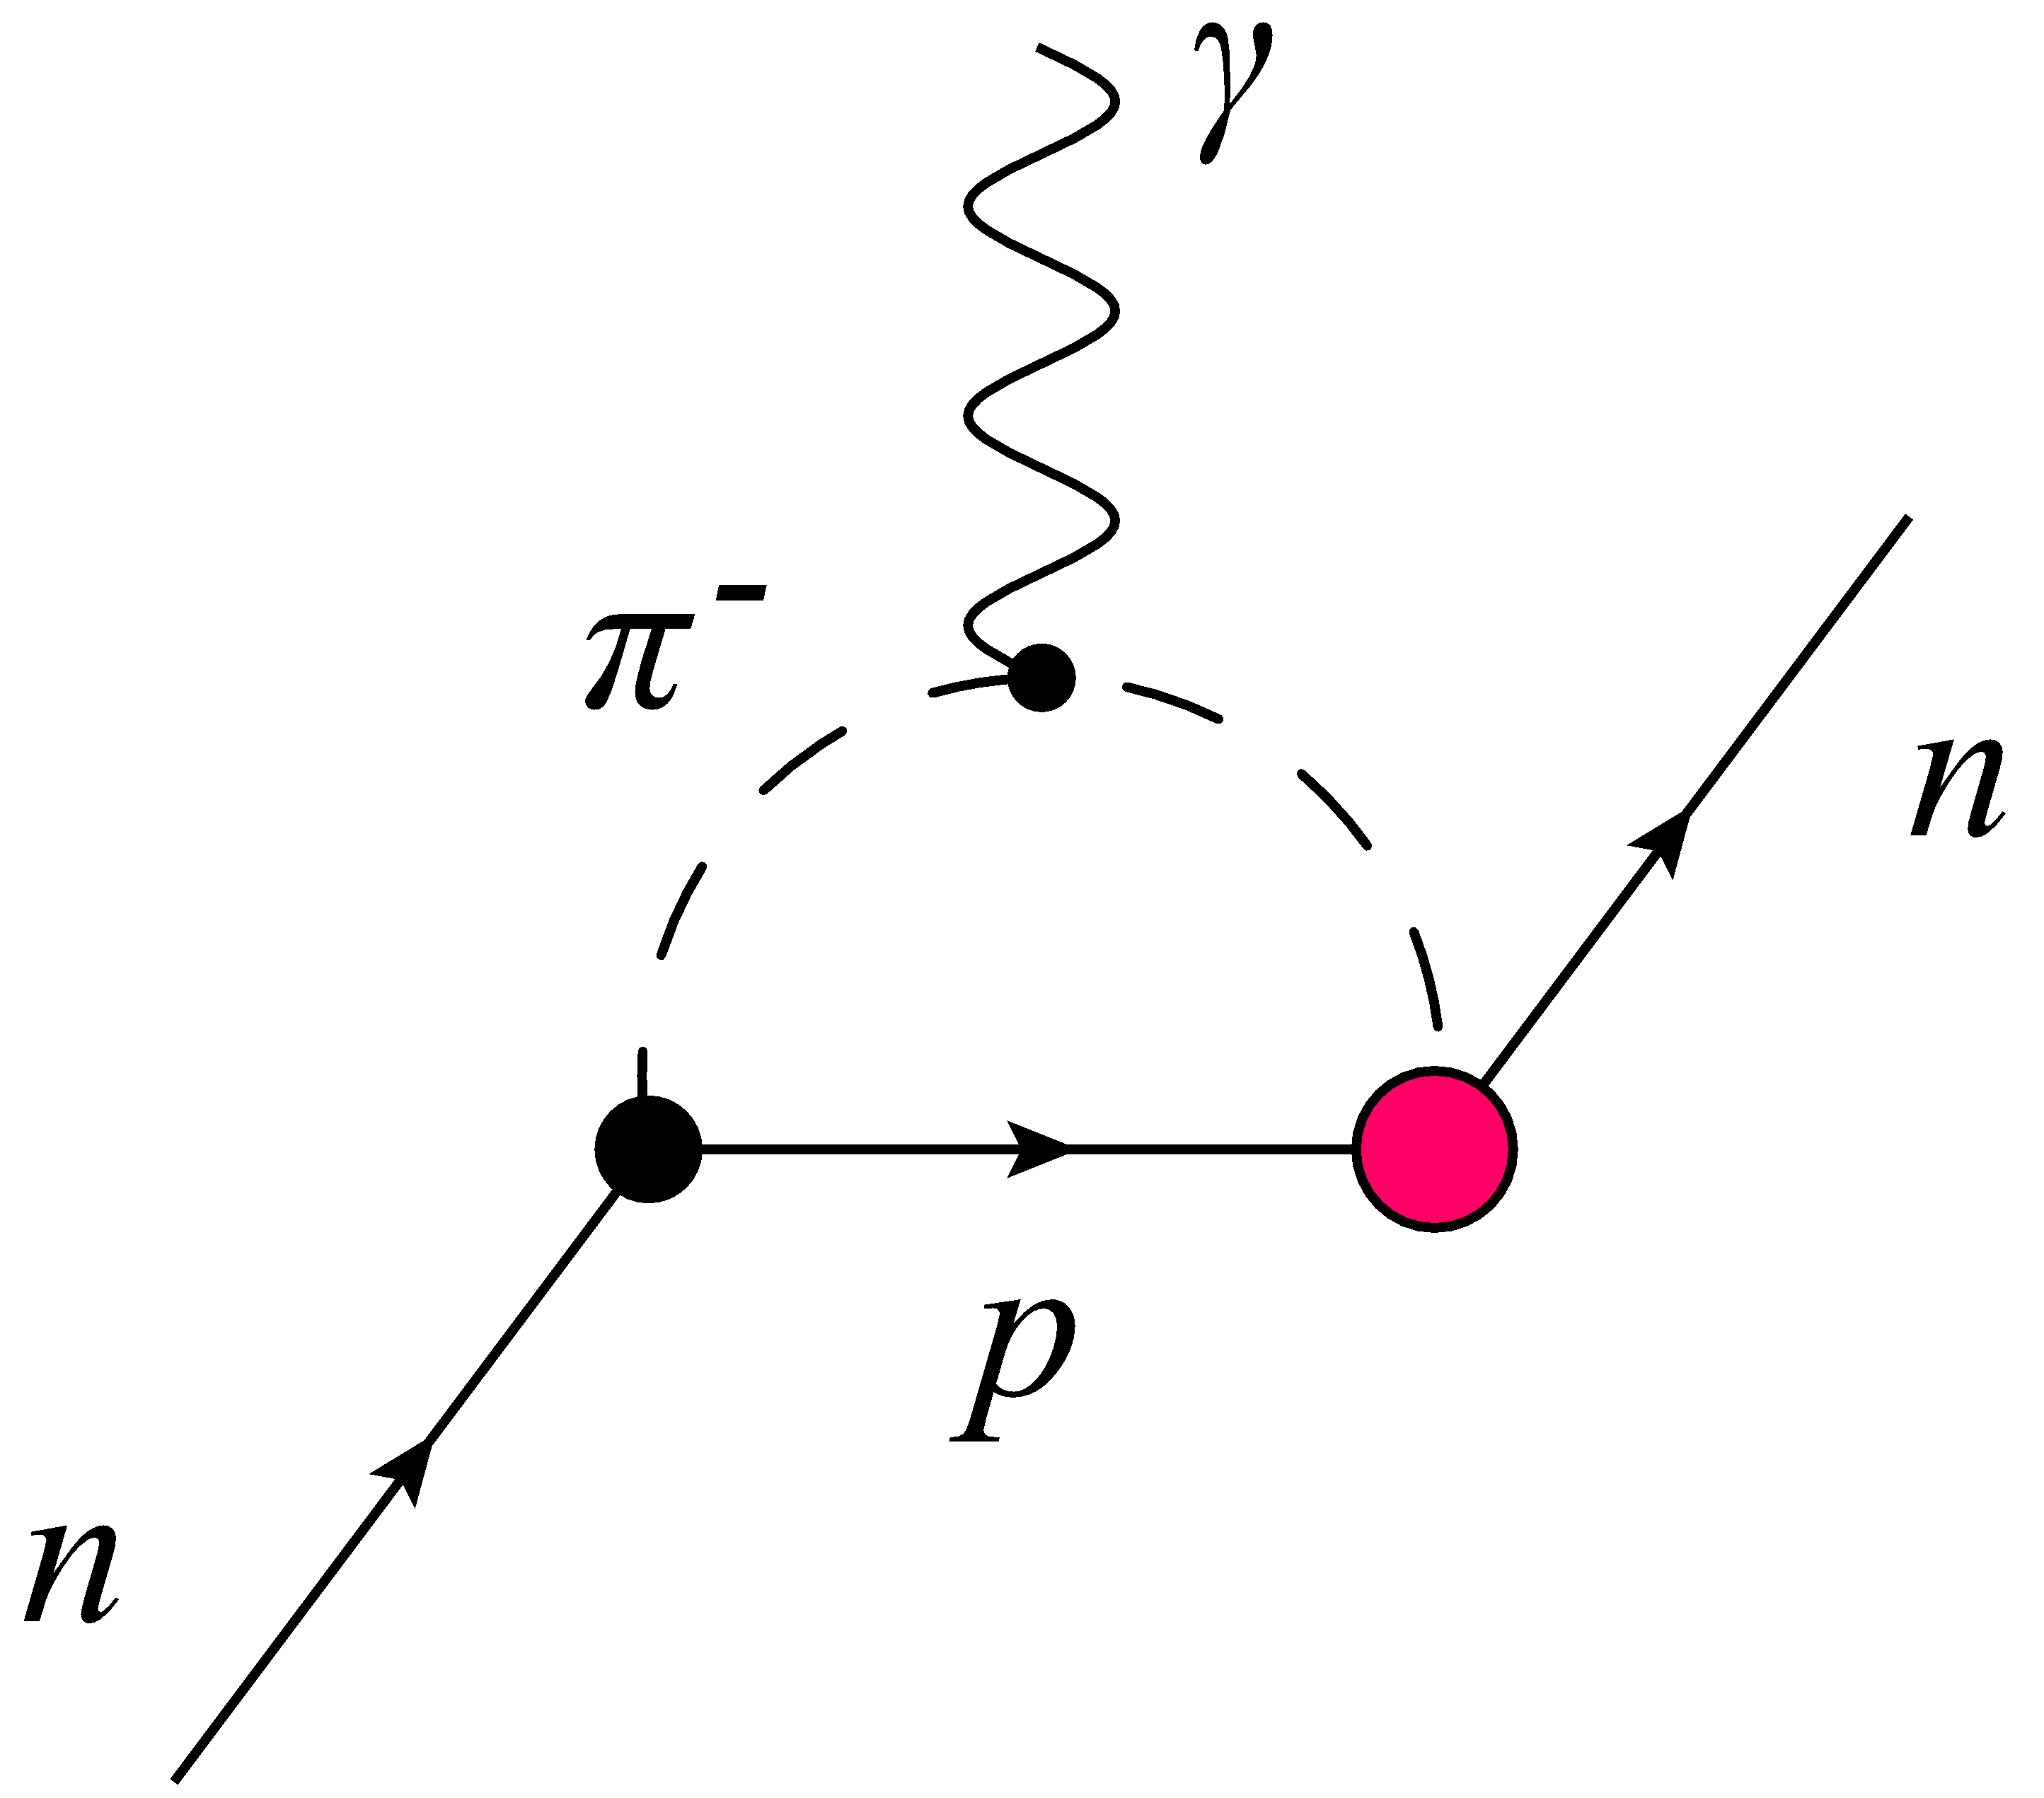
\includegraphics[width=3.3cm]{gfx/axions/nEDM_soft_pion_limit_NEW.png}
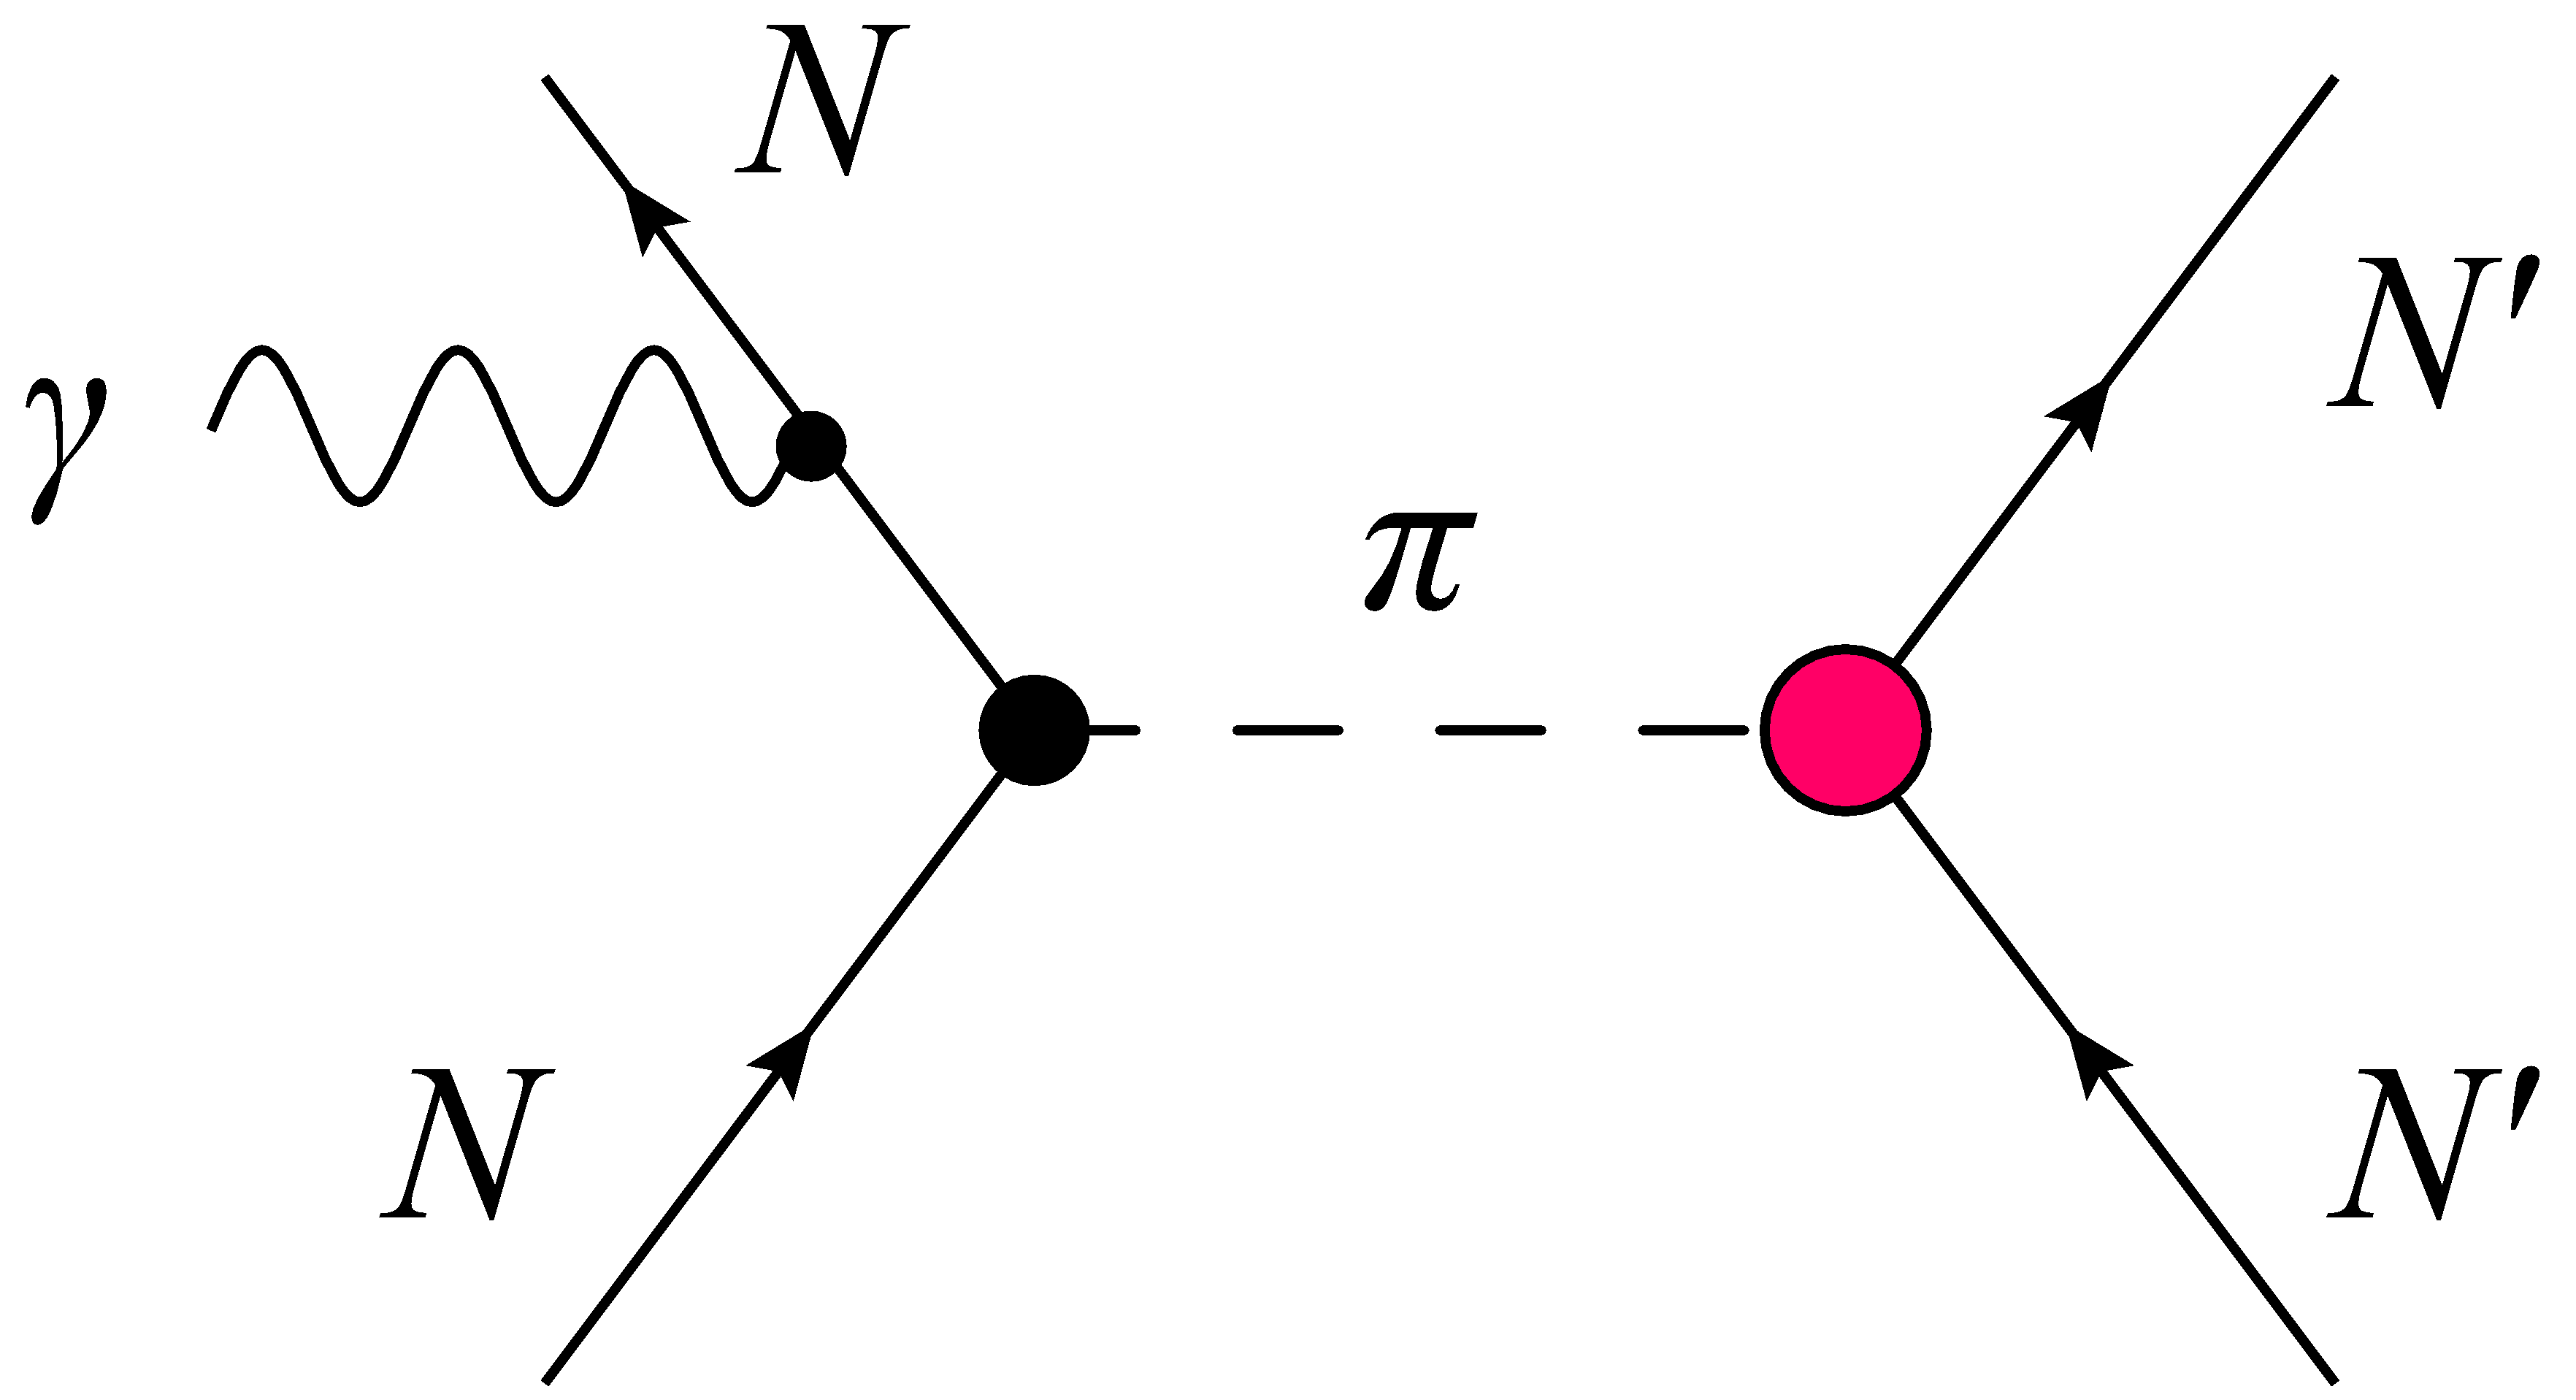
\includegraphics[width=4.1cm]{gfx/axions/Pion_nucleon_PT-odd_NEW.png}
\caption{(Color online) Fig.~1a: Process responsible for axion-induced oscillating EDMs of the free neutron and of nucleons (replace the $\pi^{-} p$ loop by a $\pi^{+} n$ loop for the proton) in atomic nuclei.
Fig.~1b: Dominant process for axion-induced oscillating P,T-violating electromagnetic moments of atomic nuclei.
Bold black circles denote the usual P,T-conserving $- i g_{\pi N N}  \bar{N}  \gamma^5 \tau^b N \pi^b$ vertex, while magenta circles denote the axion-induced P,T-violating $\bar{g}_{\pi N N}^{(0)} \bar{N} \tau^b N \pi^b$ vertex, with $g_{\pi NN} = 13.5$, $\bar{g}_{\pi N N}^{(0)} \approx 0.027 a_0/f_a \cos(m_a t)$ \cite{Witten1979} (a more recent value calculated from SU(3) chiral perturbation theory gives $\bar{g}_{\pi N N}^{(0)} =0.016 a_0/f_a \cos(m_a t)$ \cite{Mereghetti2015}), and where the sums run over the isospin index $b=1,2,3$.  }
\end{center}
\end{figure}


An oscillating galactic axion field, $a = a_0 \cos(m_a t - \vtr{p}_a \cdot \vtr{r})$, produces the following time-dependent non-relativistic potential for a spin-polarised source, via the spatial components of the second term in Eq.~(\ref{Axion_couplings}):
\begin{equation}
\label{potential_axion-wind}
H_{\textrm{int}} (t) \simeq \sum_{f=n,p,e} \frac{C_f \sqrt{\rho_{\textrm{CDM}}^{\textrm{local}} \Omega_a / \Omega_{\textrm{CDM}}}}{\sqrt{2} m_a f_a} \sin(m_a t) ~ \vtr{\sigma}_f \cdot \vtr{p}_a \, ,
\end{equation}
where we have made use of the relation $\rho_a \simeq m_a^2 a_0^2 /2$, and $\vtr{p}_a = m_a \vtr{v}_a$ is the average axion momentum relative to the Solar System ($|\vtr{v}_a| \sim 10^{-3} c$).
We evaluate the term $\vtr{\sigma}_f \cdot \vtr{p}_a$ in Eq.~(\ref{potential_axion-wind}) by transforming to a non-rotating celestial coordinate system (see, e.g., \cite{Kostelecky1999}) \note{MR: This transformation assumes a particular choice of $t=0$, as stated in Sec.\,IID of \cite{Kostelecky1999}}:
\begin{align}
\label{sigma-p_a_2}
\vtr{\sigma}_f \cdot \vtr{p}_a & = \hat{m}_F f(\sigma_f) m_a |\vtr{v}_a|  \notag \\
&\times \left[\cos(\chi) \sin(\delta) + \sin(\chi) \cos(\delta) \cos(\Omega_{\textrm{sid}} t - \eta) \right] \, ,
\end{align}
where $\chi$ is the angle between Earth's axis of rotation and the spin quantisation axis ($\chi = 44.8^\circ$ at Grenoble), $\delta \simeq -48 ^\circ$ and $\eta \simeq 138 ^\circ$ are the declination and right ascension, respectively, of the galactic DM flux relative to the Solar System \cite{NASA2014web}, $\Omega_{\textrm{sid}} = 2\pi / (23.93~\textrm{hours})$ is the daily sidereal angular frequency, $\hat{m}_F = m_F / F$, with $F$ being the total angular momentum and $m_F$ being the projection of $F$ onto the quantisation axis, and $f(\sigma_f)$ is the fermion spin-content function (see Table \ref{tab:spin-content-function-values} for the relevant values).
%\note{Notes for later: Sagnac effect and gyroscopic shift due to Earth's rotation; stability of direction of spin polarisation?}


%%%%
  \begin{table}[h!]
    \centering%
    \caption{Calculated values of the fermion spin-content function for the free neutron, $^{199}$Hg atom and $^{133}$Cs atom. We have used the calculated neutron and proton spin contributions for the $^{199}$Hg and $^{133}$Cs nuclei from \cite{Stadnik2015NMBE}.}
%\begin{tabular}%
\begin{tabular}{cccc}
\multicolumn{1}{c}{Species}   & \multicolumn{1}{c}{$f(\sigma_n) $}   & \multicolumn{1}{c}{$f(\sigma_p) $} & \multicolumn{1}{c}{$f(\sigma_e) $ }   \\
\hline
free neutron	&	1	&	0	&	0	\\
$^{199}$Hg atom	&	$-$0.30	&	$-$0.03	&	0	\\
$^{133}$Cs atom ($F=4$ state)	&	$-$0.21	&	$-$0.57	&	1	\\
$^{133}$Cs atom ($F=3$ state)	&	$-$0.20	&	$-$0.55	&	$-$0.75	\\
  \end{tabular}%
%\end{tabular}%
    \label{tab:spin-content-function-values}%
  \end{table}%.
%%%%%%%%%%







%%%%%%%%%%%%%%%%
\section{Long time--base analysis}
% \textbf{Experiment.} ---

\note{Description of experiment and analysis.}

\note{Point out that ultracold neutrons have previously been used as a sensitive probe in searches for a permanent static EDM of the neutron \cite{Baker2006,Serebrov2014,Pendlebury2015}, and for a gravitational dipole moment of the neutron, and tests of the invariance of the Lorentz and CPT symmetries \cite{Altarev2009,Altarev2010}.}

\subsection{The Sussex-RAL-ILL Room Temperature Neutron Electric Dipole Moment Experiment}
\note{NA: this subsection is still a very early draft, I know there are still formatting issues and blanks}

\note{This first bit is paraphrased from C.A. Baker et al., Apparatus for Measurement of the Electric Dipole Moment of the Neutron using a Cohabiting Atomic-Mercury Magnetometer}

\note{MR: This should probably be made much shorter.}

Most experiments to measure the static electric dipole moment of the neutron use magnetic resonance techniques to observe the Larmor precession of free neutrons in parallel and antiparallel magnetic and electric fields. The Hamiltonian of an uncharged spin $1/2$ particle in an electric and a magnetic field is:
\begin{equation}
H = - 2\vec{S} \cdot (\mu \vec{B} + d \vec{E})
\end{equation}
In the case of parallel and antiparallel magnetic and electric fields, this gives a precession frequency of:
\begin{equation}
h\nu = -2\mu B \mp 2dE
\end{equation}
In the presence of a non-zero EDM, when the direction of the applied electric field is reversed relative to the magnetic field we expect a shift in the precession frequency of
\begin{equation}
\delta \nu _0 = −\frac{4d_n E_0}{h} .
\end{equation}
In the Sussex-RAL-ILL Room Temperature experiment, polarised ultracold neutrons produced at the fundamental physics beamline at the ILL high flux reactor were stored in a material bottle (a cylinder of diameter 235mm and height 120mm), wherein their precession frequency in parallel and antiparallel combinations of electric and magnetic fields was measured using the Ramsey Technique. To combat drifts in the magnitude of the applied magnetic field, a cohabiting magnetometer of atomic $^{199}$Hg was used, and analysis was done by considering the ratio of neutron and mercury precession frequencies, “$R$”.

Each measurement sequence (“cycle”) consisted of a filling period, a first $\pi/2$ pulse to rotate the neutron spins into the horizontal plane, a 130s period of free precession, a second $\pi/2$ pulse to project the spins onto the z axis, and an emptying period where the number of spin-up and spin-down neutrons were counted. The precession of the mercury during the free precession period was measured by observing the modulation of the absorption of light from a mercury discharge lamp \note{is it actually a discharge lamp?}. Each cycle lasted in total x minutes. Many cycles were taken at each fixed magnetic field configuration over the course of between 1 and 73 hours (a “run”), while the direction of the applied electric field was reversed every 20 cycles. From each run a value of the neutron to mercury frequency ratio $R$ was extracted, as well as a value of the apparent EDM.

As a result of a conspiracy between radial magnetic field components and rotating magnetic components arising from the Lorentz transformation of the large applied electric field into the rest frame of the mercury atoms, a frequency shift proportional to the applied electric field was observed, mimicking the effect of a non-zero electric dipole moment of the neutron --- a “false EDM”. This effect is, however, directly proportional to the gradient of the applied vertical magnetic field dBz/dz, and reverses with the sign of the applied magnetic field. The false EDM effect has been analysed in more detail in \note{cite false edm paper(s)} and a direct measurement of this effect was made in \note{cite false edm measurement}.

As the ILL experiment had no direct measurement of the vertical gradient, the measurement of the neutron to mercury frequency ratio was instead used as a proxy. Due to the extremely low energy of the ultracold neutron population, the centre of mass of the neutron population sags a little below the centre of the precession chamber. The relatively hot population of mercury atoms does not suffer from this effect, so there is an effective height difference $\Delta h \approx 3.7 \mathrm{mm}$ between the neutron and mercury populations. Thus, the ratio of neutron to mercury frequencies depends (to first order) on the vertical gradient like: \note{MR: We might want to get rid of the stacked fraction for clarity.}
\begin{equation}
  R = R_0 \left( 1 + \Delta h  \frac{\frac{\mathrm{d}B_z}{\mathrm{d}z}}{B_{0}} \right).
  \label{eq:R}
\end{equation}
This frequency shift does not uniformly affect the entire neutron population: the effect is much greater for the lowest energy neutrons which have a lower centre of mass. This causes a departure from the linear relation above; however, in the low vertical gradient regime ($\lesssim 30 \mathrm{pT/cm}$) in which most of the data was taken, the effect is almost exactly linear. This effect is described more thoroughly in [cite grav depol papers].

To correct for these false EDMs in static EDM searches, the “crossing lines” procedure was adopted.  For each direction of the magnetic field, the measured EDM value was plotted against the measured neutron to mercury frequency ratio. Barring other systematic shifts, it is considered that the vertical gradient is zero where these lines cross. Other effects arising from transverse magnetic fields, the rotation of the earth and cause additional frequency shifts in the neutrons or in the cohabiting magnetometer, which can \note{PH: no it isn't -- there are still systematics from e.g. transverse fields, which can move the crossing point away from dB/dz=0, in addition to effects such as Earth's rotation that result in a vertical shift of the crossing point...]}, and therefore a measurement of the neutron electric dipole moment independent of the false EDM effect and of the neutron to mercury frequency ratio independent of the gravitational shift can be extracted. In the rest of the run-level analysis, we work with data where these false EDM effects have been subtracted. Further systematic effects shift the measured neutron to mercury frequency ratio or the measured EDM value, however these effects can be assumed to have been constant throughout the entire experimental measurement period, and so will not be further explored in this analysis. Systematic effects affecting the static analysis of the ILL experiment are explored in depth in [cite reanalysis] and [cite apparatus paper].

\note{MR: Need to mention explicitly, that the average $d_n$ over a run is measured (though not exactly, it is only over the free precession periods), and this is how it is treated in the Monte Carlo simulations.}

% \subsection{Analysis strategy}
% We are looking for oscillations in the neutron EDM value $d_n$. Our analysis is split into two distinct parts. Firstly, we perform a Run--Level analysis using the Sussex--RAL--ILL data. There we are looking for time series...
% MR: moved to the introduction

\subsection{Least Squares Spectral Analysis}
In this section, we present the statistical methods we use. We start by defining the \emph{periodogram}, which serves as a transition from time to the frequency space, natural for looking for oscillations. Next we proceed to discuss the statistical properties of the periodogram, which lays the basis for this analysis.

A \emph{periodogram} is an estimator of the power spectrum. With the Least Squares Spectral Analysis (LSSA) method one can construct a statistically well--behaving periodogram for non-uniformly sampled data with unequal error--bars. To evaluate the LSSA periodogram at a circular frequency $\omega$, one performs a linear least--squares fit (hence the name) to the data with a function
\begin{equation}
  A\,\mathrm{cos}(\omega t) + B\,\mathrm{sin}(\omega t) + C \ ,
\end{equation}
where $A$, $B$ and $C$ are free parameters. The estimator of power $P(\omega)$ is then defined as
\begin{equation}
  P(\omega) := \frac{N}{4} \, \left( A^2 + B^2 \right) \ ,
\end{equation}
where $N$ is the number of data points. Different scaling factors may be used. We use the one of \cite{Scargle1982}, where the height of $\sqrt{P(\omega)}$ at the noise--bed corresponds numerically to the size of the error--bars squared, if they are all equal. LSSA, in contrast to FFT, does not require windowing, because it is explicitly phase--aware. A graphical overview of the method is shown in Fig.\,\ref{fig:LSSA}. Throughout the analysis, the figure of merit is either the power $P(\omega)$ or, interchangeably, its square root \emph{amplitude}. \note{MR: for clarity we may always speak of power (or only of amplitude) --- would need to decide which is better. I'd say to use amplitude, as it has more intuitive units.}

\begin{figure}[htb]
  \centering 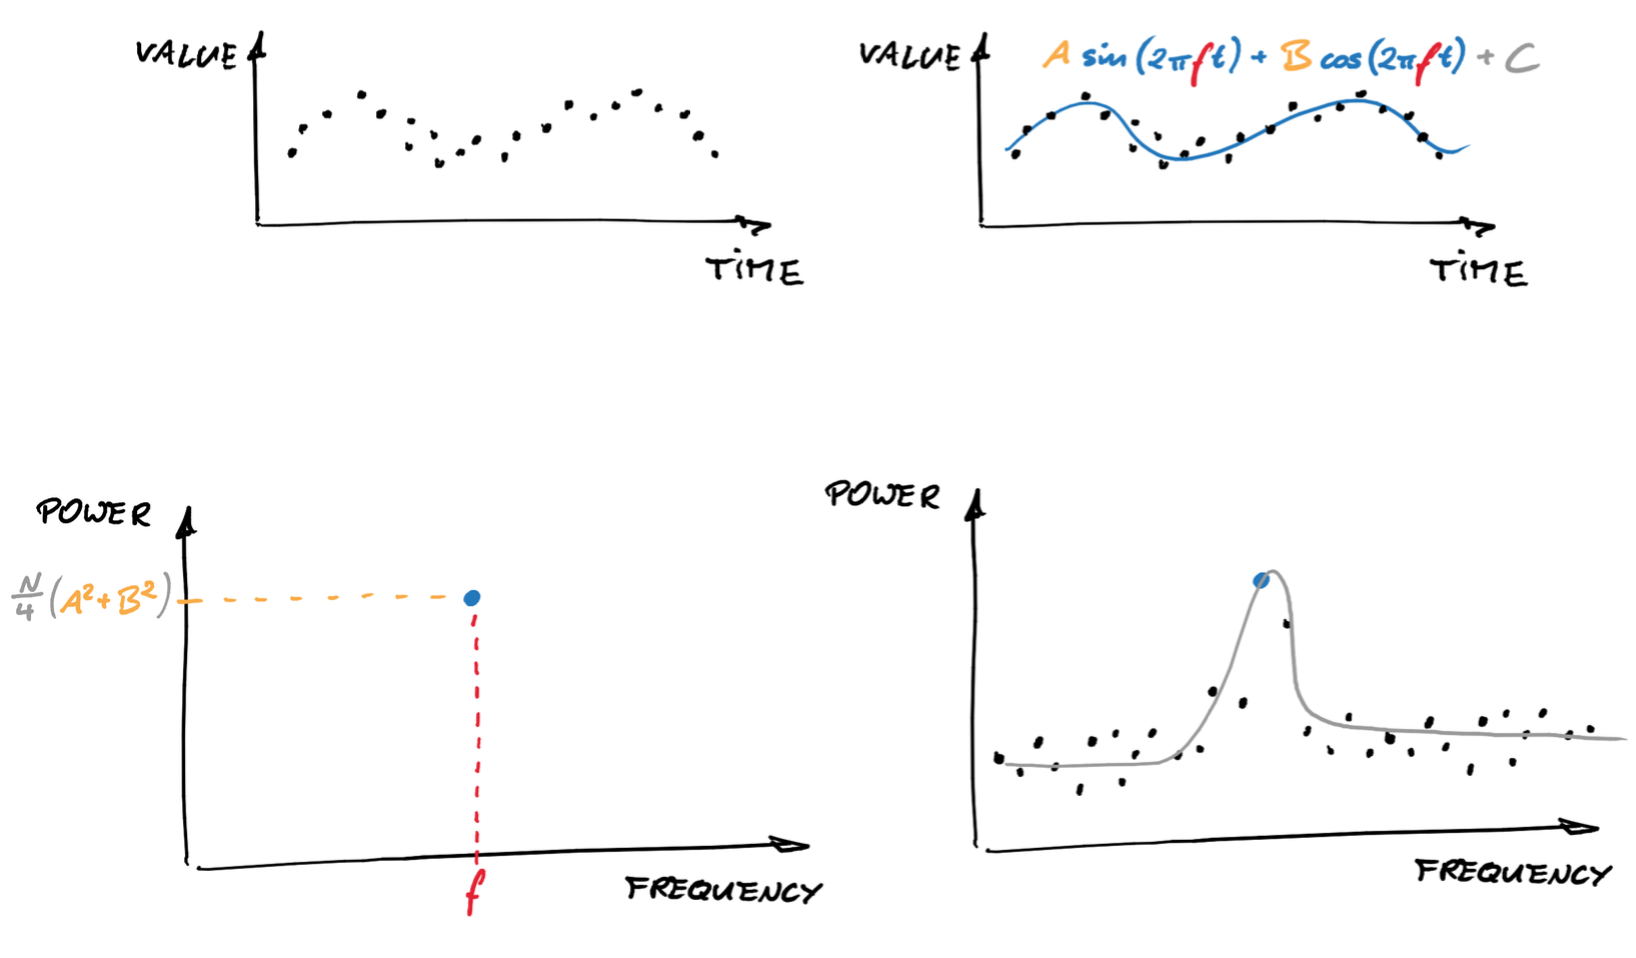
\includegraphics[width=\linewidth]{gfx/axions/LSSA}
  \caption{The LSSA periodogram, a function of frequency, is constructed by performing a linear least--squares fit at each of those frequencies.}
  \label{fig:LSSA}
\end{figure}


\subsection{Choice of frequencies}
The LSSA periodogram can be evaluated at any frequency. We are going to motivate the choice of a set of frequencies.

Every kind of spectral analysis is fundamentally limited by \emph{spectral resolution} (also referred to as \emph{bandwidth resolution}), which is approximately equal to the inverse time separation between the first and the last measurement. If the LSSA power is evaluated more densely than that, the results are expected to be highly correlated. Additionally, if the LSSA periodogram stretches beyond approximately half of the sampling frequency \note{MR: sampling frequency is not even well defined in our case}, following the reasoning similar to the Nyquist--Shannon sampling theorem \note{MR: citation needed?}, aliasing is expected to occur, introducing correlations between points of the periodogram.

We do not make special effort to avoid sampling frequencies where spurious power fluctuations will be correlated. An exact treatment of the correlations is virtually impossible in our complicated case, when the measurements are neither equally--spaced nor point--like. We prefer to take the possible correlations into account, which gives us freedom when it comes to choosing the frequencies.

We want to choose the frequencies, such that (a) we cover a broad spectrum and (b) we are sure to detect an axion--induced peak, if it is in the covered spectrum. The coherence of the oscillating axion field is of the order of $10^6$ periods, which translates into a relative width of the peak they would produce in the periodogram of $10^{-6}$. The spectral resolution of the ILL data set is the inverse of 1545 days ($\approx \unit[7.5 \cdot 10^{-9}]{Hz}$), which means that above frequencies of above $\unit[7.5 \cdot 10^{-3}]{Hz}$ the width of the peak is not resolvable. As we do not attempt to stretch beyond this frequency, the spacing between frequencies has to be at most equal to the spectral resolution.

As the highest frequency we choose approximately 10 times per day ($\unit[10^{-4}]{Hz}$) \note{MR: to be filled by NA}. We have one data point approximately every day. For frequencies higher than that, the sensitivity quickly drops and the computational needs rise. We cover the space between zero (exclusive) and the highest frequency with linearly spaced frequencies separated by one spectral resolution. This gives us $\sim 10^6$ frequencies to analyse. In order to stretch our results in the low--frequency direction, we add 100 logarithmically spaced frequencies below one spectral resolution. As the lowest frequency we choose the frequency that would correspond to an axionlike particle of mass $\unit[10^{-24}]{eV}$ ($\unit[9.54 \cdot 10^ {-9}]{Hz}$) \note{MR: to be filled precisely by NA}. \note{YS: Shouldn't the inverse of 20 years correspond to a much smaller frequency, or are we talking about something different here? NA: inverse of 20 years should be much less than $10^-4$Hz, I have changed to show the actual lowest frequency I use. I have justified it in terms of axion mass, but maybe if we are presenting a limit on oscillating EDMs with an interpretation in terms of alp couplings we should use a different justification or lower frequency} Thereby a set of $N$ angular frequencies $\omega_i$ is constructed.


\subsection{Null hypothesis test}
In the run--level analysis, the time series is the neutron electric dipole moment $d_n$ measured in each run of the ILL experiment. We calculate the LSSA periodogram of this series. A signature of an oscillating signal would be a peak in the periodogram. Precisely, we want to answer the question:

\begin{center}
  \emph{How likely is it that the highest peak in the periodogram is not only a random fluctuation?}
\end{center}

We are, in fact, interested in the \emph{least likely} peak, which may not be equivalent to the highest one. For clarity we are going to be first considering the highest peak, and explain the difference later.\note{NA: in final PRL we should probably dive straight in talking about the least likely peak.}

To describe the question mathematically, let us denote the time series of the real data by $D$. The peridogoram is then a set of $P^D(\omega_i)$. We are interested in \emph{the maximum of the periodogram}:
\begin{align}
  P_{max}^D &:= \mathrm{max}_i\,P^D(\omega_i) \\
  \omega_{max}^D &:= \mathrm{arg\,max}_{\omega_i}\,P^D(\omega_i)
\end{align}
The height of the maximum, $P_{max}^D$, is a statistic itself. We refer to it as \emph{global}, in contrast with the \emph{local} statistics $P^D(\omega_i)$. We consider the distribution of $P_{max}^{H_0}$ given the null hypothesis $H_0$, where the time array is an array of normally distributed random variables, with widths equal to the corresponding error--bars. The probability that a peak at least as high as the one observed arises as a random fluctuation is:
\begin{equation}
  % \mathrm{Pr}\left( P_{max}^{H_0} > P_{max}^D\ |\, H_0 \right) \ .
  \mathrm{Pr}\left( P_{max}^{H_0} > P_{max}^D \right) \ .
\end{equation}
This value is called the \emph{false alarm probability} (see eg. \cite{Pandola2004}). It can be numerically calculated with the Monte Carlo method by generating random data according to the null hypothesis (Fig.\,\ref{fig:generating_null_hypothesis_periodogram}) and counting the relative number of cases when $P_{max}^{H_0} > P_{max}^D$. To claim a discovery, the \emph{false alarm probability} has to be at most in the range of $2.87\,\cdot\,10^{-7}$ (so--called 5--sigma) \cite{PDG2014}.

\begin{figure}[htb]
  \centering 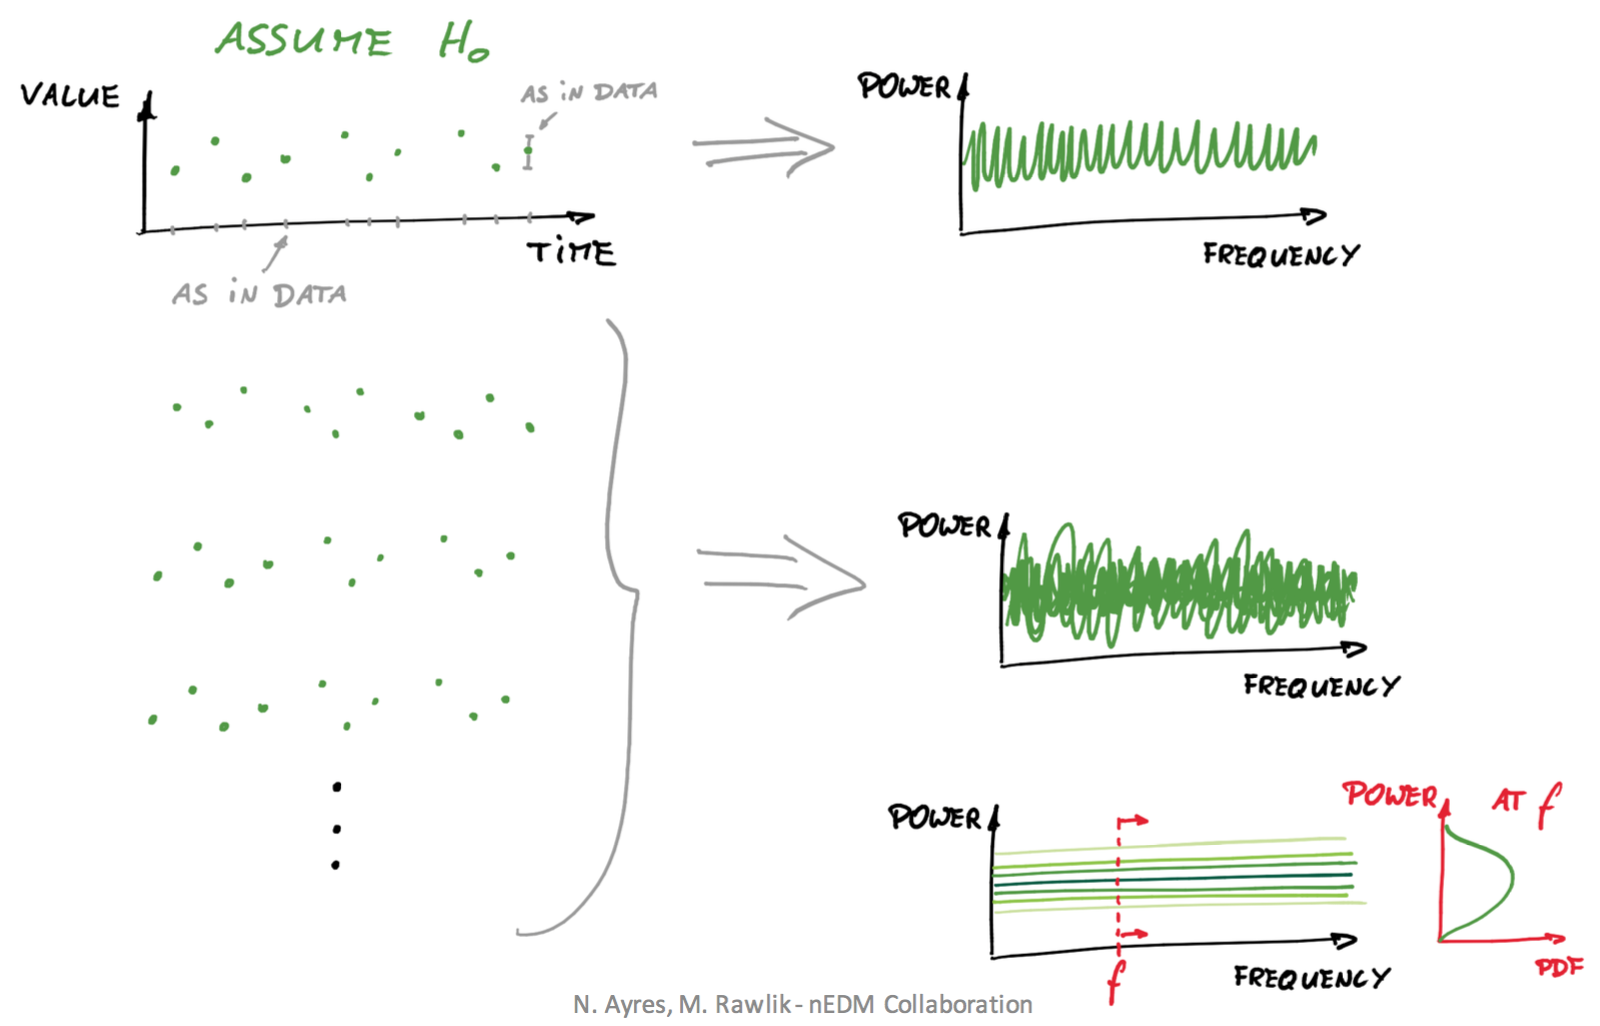
\includegraphics[width=\linewidth]{gfx/axions/null_hypothesis.png}
  \caption{The distrbution of LSSA periodogram for the null hypothesis is generated with a Monte--Carlo method. As the periodogram is a one--dimensional function, its distribution is two--dimensional.}
  \label{fig:generating_null_hypothesis_periodogram}
\end{figure}

It should be stressed that the distribution of $P_{max}$ is very different from the one of $P(\omega_{max})$. By looking for the highest peak, we check a big number of random variables $P(\omega_i)$ and pick a very special one --- the one that does lie the furthest in the tail of the distribution. The distribution of $P_{max}$ thus is centred around much higher values, as shown in Fig.\,\ref{fig:max_power_distribution}.

\begin{figure}[htb]
  \centering 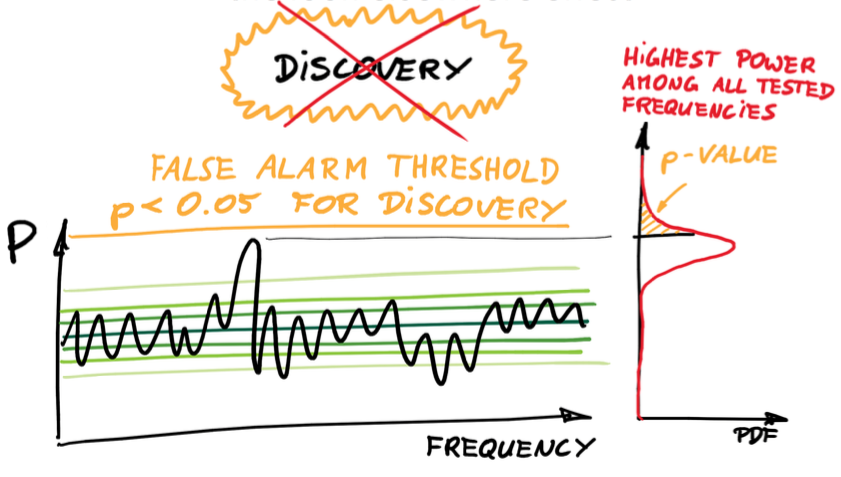
\includegraphics[width=\linewidth]{gfx/axions/max_power_distribution.png}
  \caption{The distribution of \emph{highest power} in a periodogram is centered much higher then the distributions of power in the periodogram.}
  \label{fig:max_power_distribution}
\end{figure}

\note{MR: might consider a better notation} As already mentioned, we are really interested in the \emph{least--likely} peak. Only if the noise--bed (the null hypothesis periodogram) is flat, then the highest peak corresponds to the least--likely peak. The cumulative distribution function (CDF) of power at frequency $\omega_i$ can be estimated by evaluating $P(\omega_i)$, $P_i$ for short, for many signals generated assuming $H_0$. We denote the CDF by $F_{P_i}$. The \emph{local} p-value for the compatibility of $P^D(\omega_i)$ with $H_0$ is simply:
\begin{equation}
  p_i = 1 - F_{P_i}(P^D_i)
\end{equation}
The \emph{local} p-value for the least--likely peak is:
\begin{equation}
  p_{\mathrm{min}} = \mathrm{min}_i \, p_i
\end{equation}

The question is what is the \emph{global} p-value of the least likely peak in the data--set being compatible with $H_0$. If the points of the periodogram were not correlated, this would be a simple case of many hypothesis testing \cite{Algeri2016}. The local p-values $p_i$ are, by definition, uniformly distributed. The CDF of a maximum of a set of uncorrelated variables is a product of their CDFs \note{MR: Cite Papoulis 1965, 7.1, application 3 - taken from Scargle III a)}. So in this case we have:
\begin{align}
  F_p(p) &= p \\
  F_{p_{max}}(p) &= p^N \\
  &\text{with}\ p' := 1 - p :\\
  F_{p_{min}}(p) &= 1 - F_{p'_{max}}(p') = 1 - (1 - p)^N \label{eq:Fpmin}\\
\end{align}
where $N$ is the number of frequencies. Correlations in the periodogram effectively lower $N$. If three dice are rolled in a way that two always give the same result, this is the same as rolling two dice when minimum roll is concerned. To quantify that, we exploit the fact that we can do fast Monte Carlo and \emph{simulate} the whole process: generating many signals assuming the null--hypothesis and calculating the p-value of the least--likely peak. Thereby we can estimate the CDF of $p_{\mathrm{min}} \, | H_0$, which we call $F^g$. Then the \emph{global} p-value is given by:
\begin{equation}
  p^g = F^g(p_{\mathrm{min}}^D)
\end{equation}

We can further determine \emph{false--alarm} thresholds. Traditionally, they are chosen to be at p-values of the normal distribution at $n \,\sigma$. The \emph{global} threshold p-value we call $p^g_{f.a.}$. The \emph{local} threshold p-value is:
\begin{equation}
  p_{f.a.} = \left( F^g \right)^{-1}(p^g_{f.a.})
\end{equation}
For each frequency the threshold power can be calculated:
\begin{equation}
  P^{f.a}_i = F_{P_i}^{-1}(1 - p_{f.a.})
\end{equation}
We claim a statistically significant discovery if the periodogram of the $d_n$ time--series crosses the 5--sigma false--alarm threshold.

The amount of Monte Carlo samples can be reduced, if the CDFs can be extrapolated. Effects like unequal error--bars and measurements of non--negligible duration causes them to deviate from the strictly derived equations in \cite{Scargle1982}. Nevertheless, we assume that functional form of the tails is preserved. Under the null hypothesis $F_{P_i}$ has form $1 - e^{-P}$ \cite{Scargle1982}. For $F^g$ we assume a form of Eq.\,(\ref{eq:Fpmin}), where $N$ is a parameter that we have to fit to account for correlations in the periodogram.

In Fig.\,\ref{fig:ILL_detection} we present the periodogram of a fake ILL dataset (geneated with the same run timings and uncertainties as in the real dataset, with run EDM values generated according to gaussian distribution with mean of $0$ and standard deviation equal to that run's uncertainty). We decided not to analyse the real data set until we are fully happy with the method.

\begin{figure}[h!]
  \begin{center}
    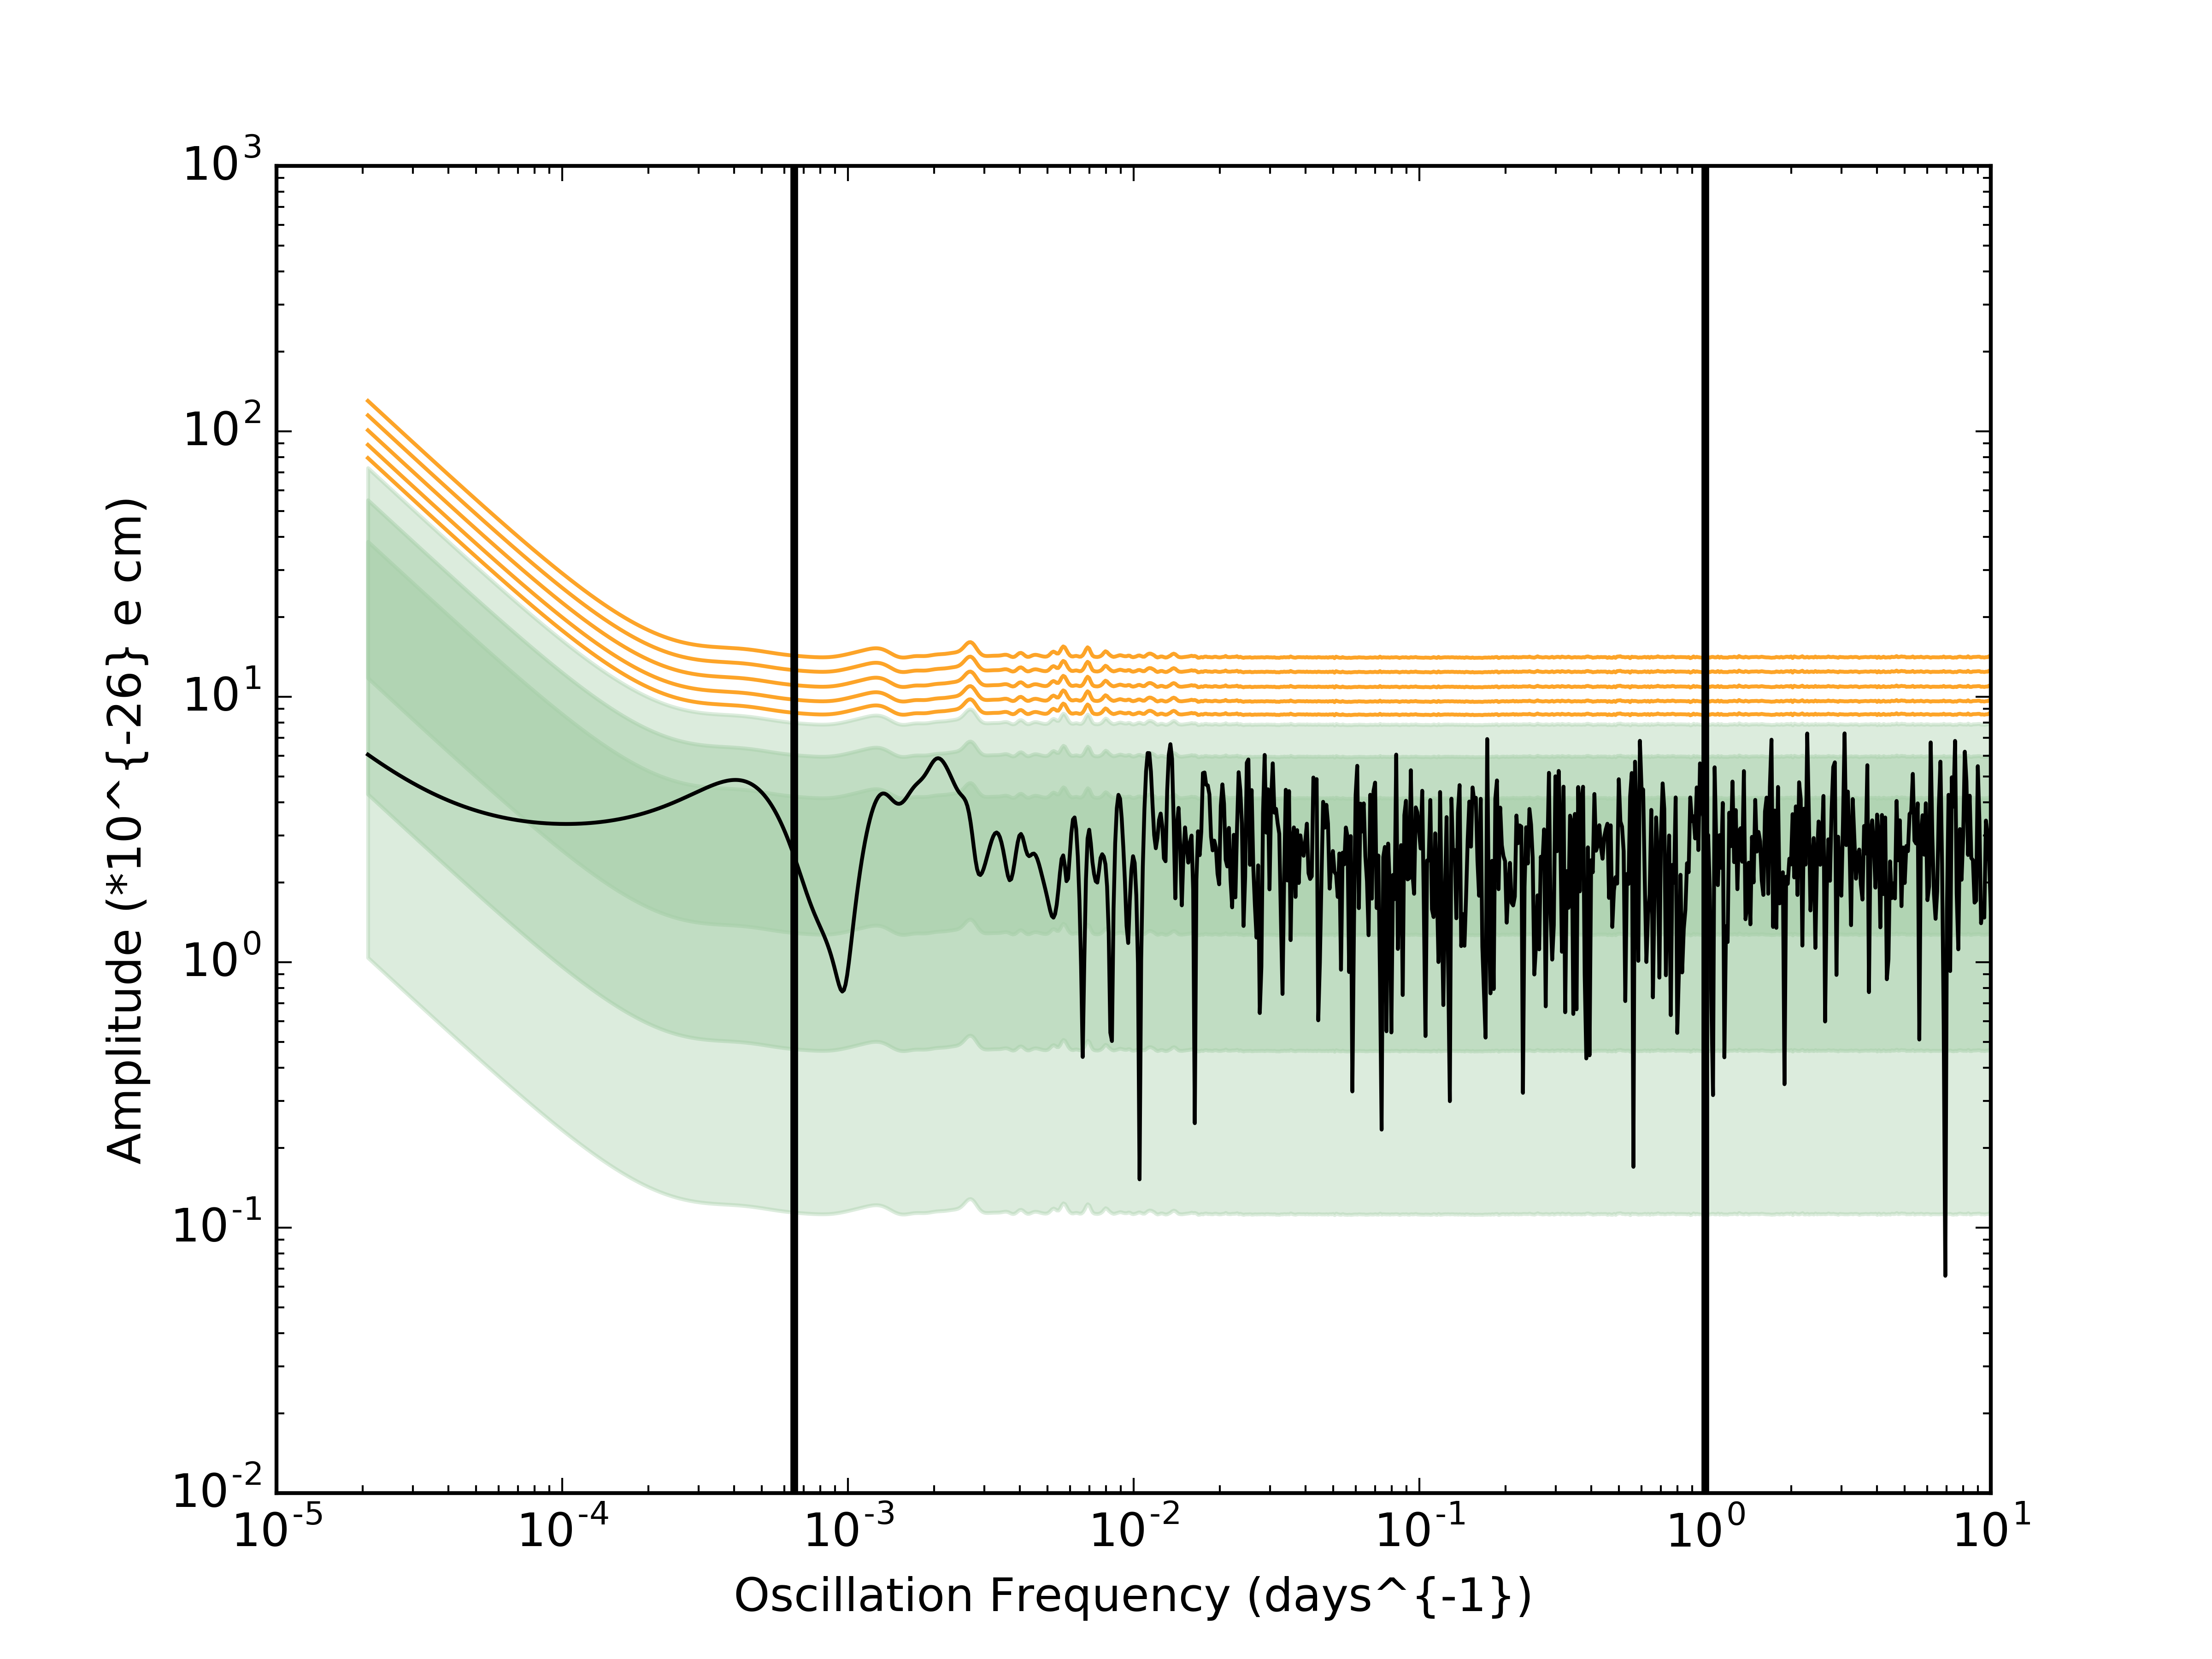
\includegraphics[width=\columnwidth]{gfx/axions/ILL_detection_Periodogram.png}
    \caption{Periodogram of a fake ILL dataset. The green bands represent the distribution of the periodogram given the null hypothesis. The orange lines are 1-, 2-, 3-, 4-, 5--sigma false--alarm thresholds.}
    \label{fig:ILL_detection}
  \end{center}
\end{figure}

\note{MR: here should go the discussion of the result.}


\subsection{Exclusion region}
\begin{figure}[htb]
  \centering 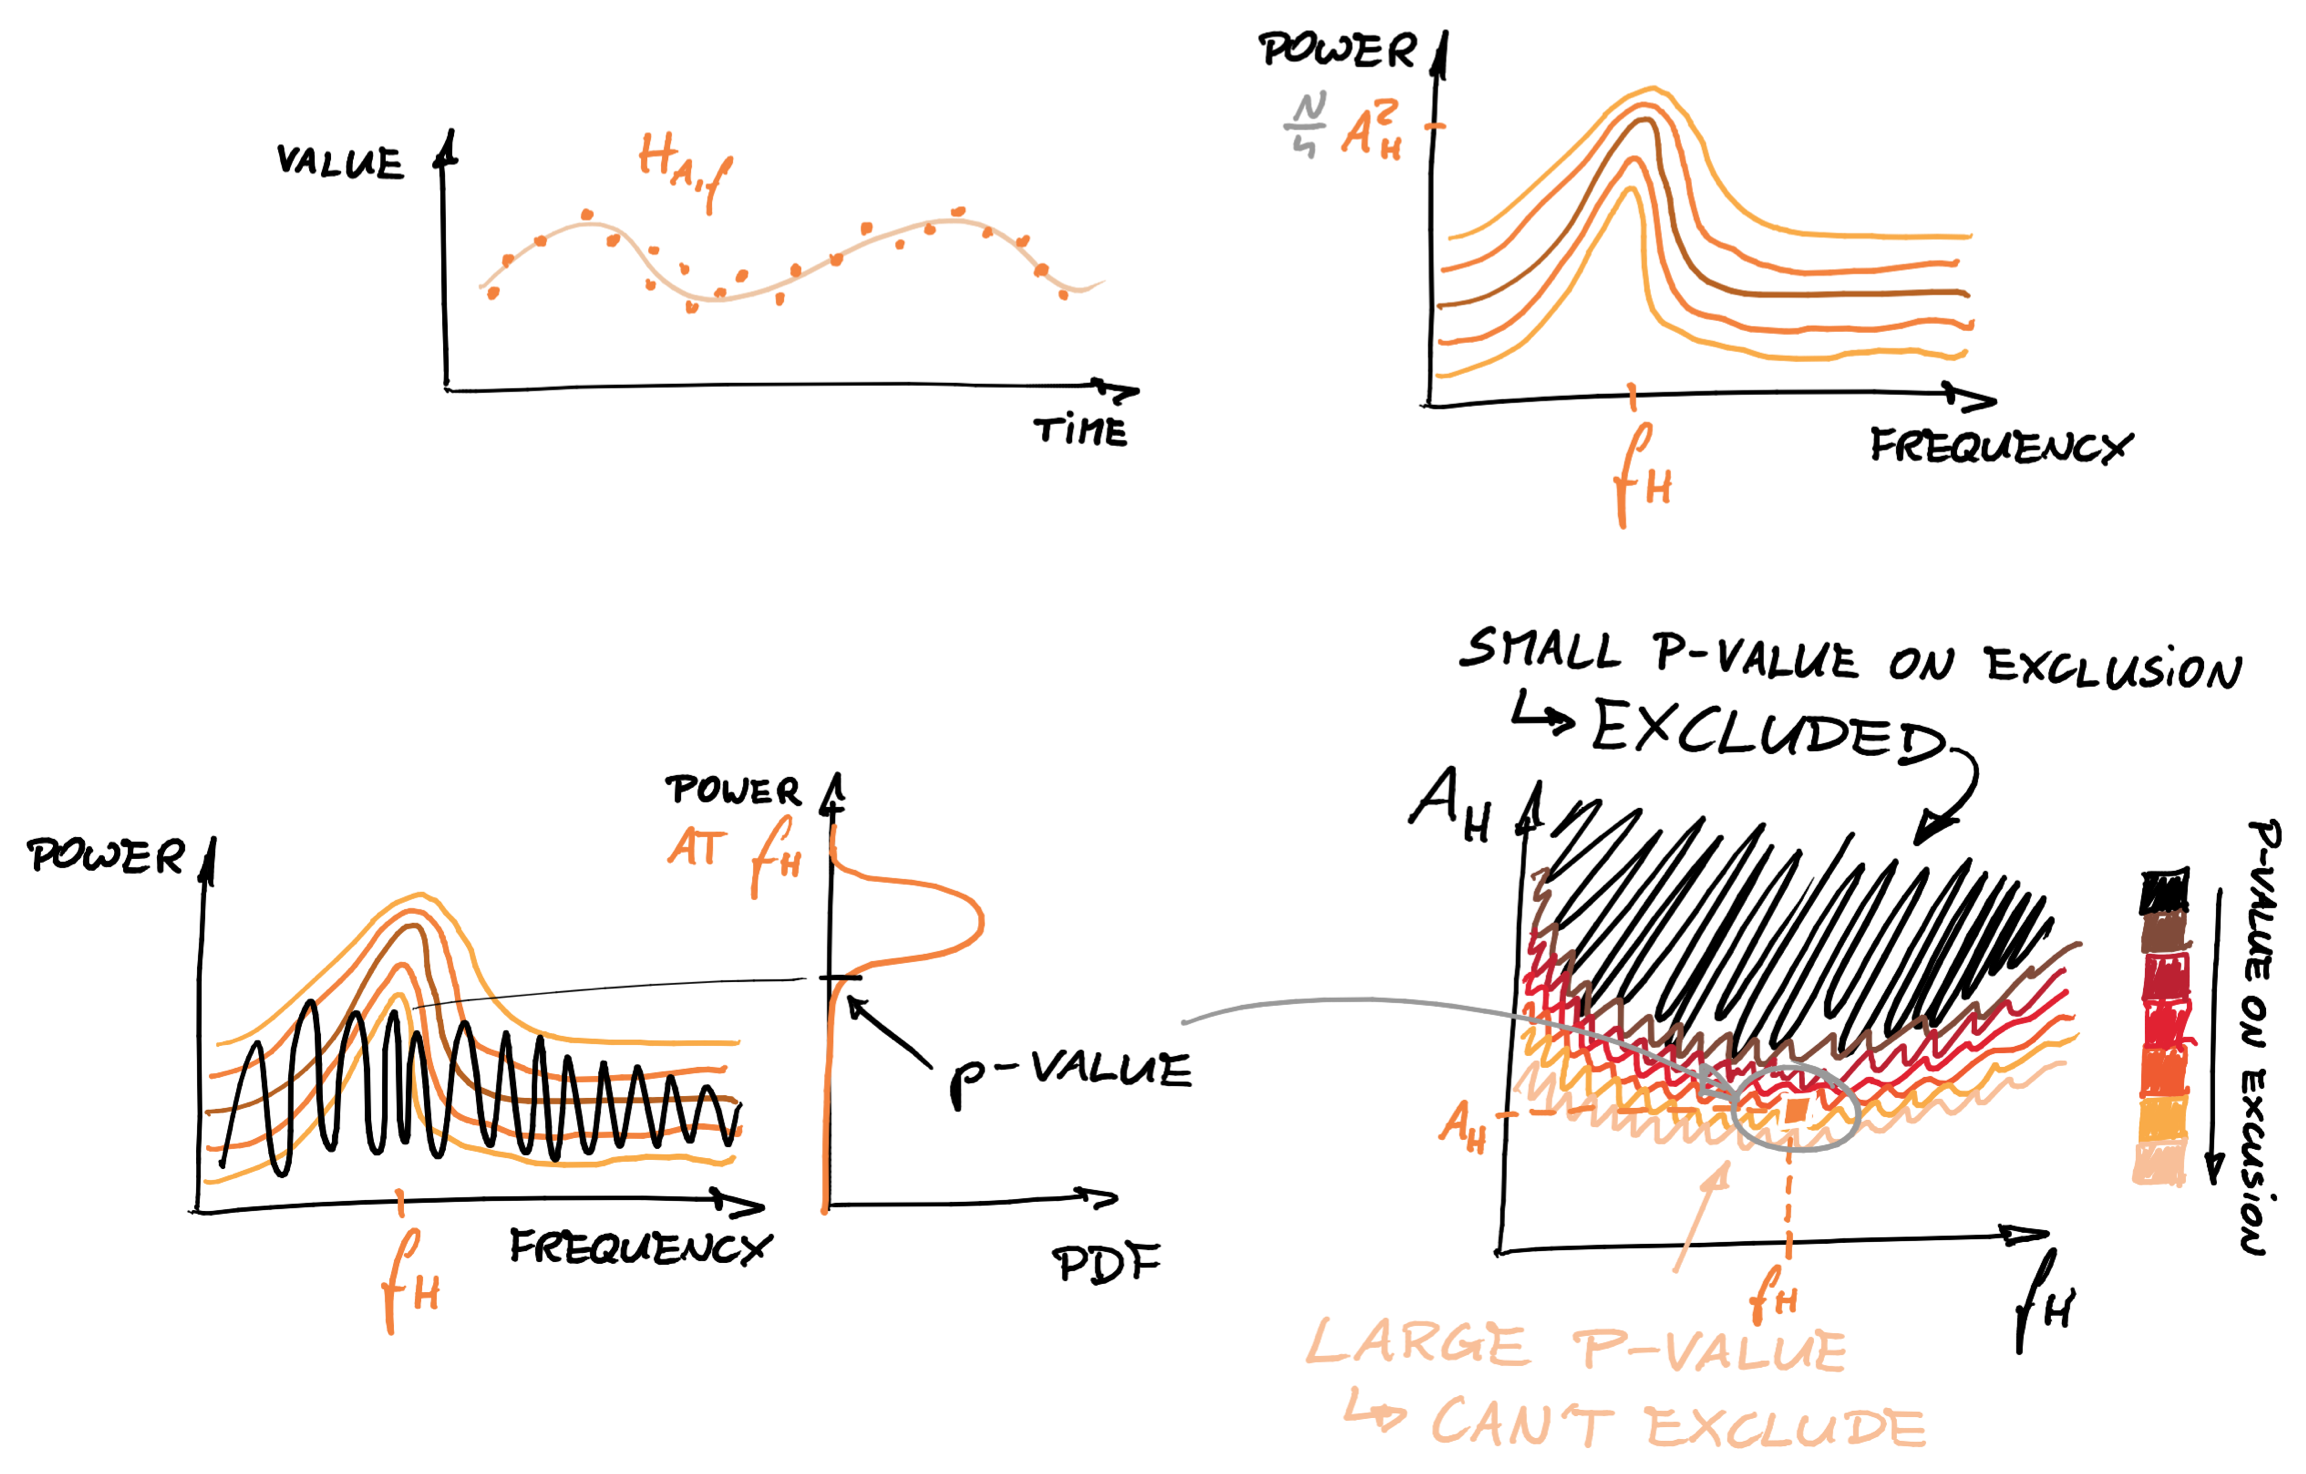
\includegraphics[width=\linewidth]{gfx/axions/exclusion_region.png}
  \caption{Determining the exclusion limit. Note that in practice not the whole periodogram needs to be generated, but only its slice at $f_H$.}
  \label{fig:exclusion_region}
\end{figure}

Should no claim for a discovery be possible, the next question to ask is:
\begin{center}
  \emph{Which oscillations would produce a significant peak, but did not, and can be thus excluded?}
\end{center}
In order to answer this question, the data need to be tested against being compatible with a number of model signal hypotheses. As an oscillation is characterised by its amplitude and frequency, the space of the alternative hypotheses to test is two--dimensional.

The probability that a hypothetical oscillation of amplitude $A$ and frequency $\omega$ would produce less power at frequency $\omega$ then observed is:
\begin{equation}
  % \mathrm{Pr}\left( P(\omega) < P^D(\omega)\ |\, H(\omega, A) \right) \ .
  \mathrm{Pr}\left( P^{H(\omega, A)}(\omega) < P^D(\omega)\ \right) \ .
\end{equation}
This probability is the p-value for the hypothesis $H(\omega, A)$ rejection. The distribution of $P^{H(\omega, A)}(\omega)$ is obtained with the Monte Carlo method. Here we also make use of CDF tail extrapolation \note{MR: This time, however, we extrapolate the low-power tail}, assuming a functional form as eq.\,(15) in \cite{Scargle1982} \note{MR: Not strictly, though. This equation behaves like linear function for very small $z$}. This test is repeated for different $\omega$ and $A$, each time covering a \emph{pixel} of the space of possible hypotheses. This procedure is shown schematically in Fig.\,\ref{fig:exclusion_region}. The set of hypotheses excluded at most at certain p-value forms an \emph{exclusion region}. We take the threshold p-value to be 5\%, which corresponds to a traditional confidence level of 95\%.

In this case, we cover the frequency spectrum much less densely than is the case in the null hypothesis test. This procedure is essentially evaluating the sensitivity of the measurement, which is solely determined by the timing and precision of the measurement points. We do not expect any highly resonant structures to appear therein.

During the Monte Carlo simulations we assume a perfectly coherent signal. The width of a real peak is not resolvable, as already mentioned.

\begin{figure}[htb]
  \begin{center}
    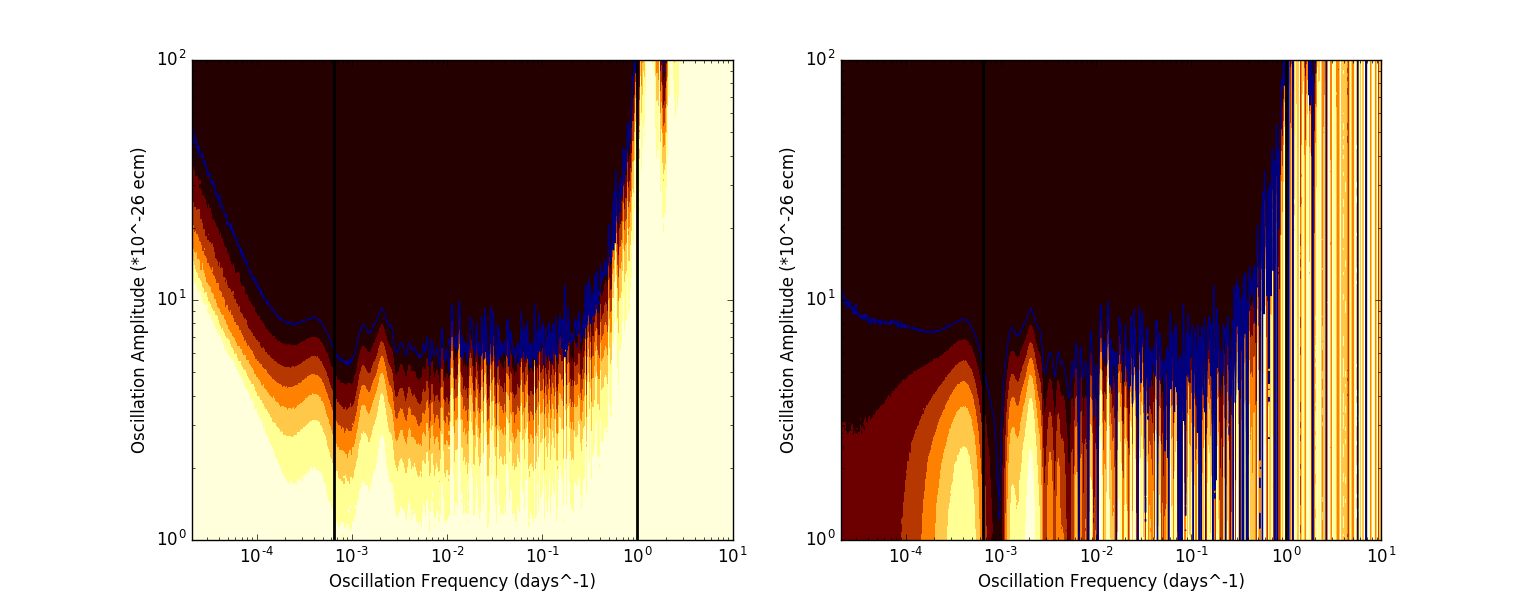
\includegraphics[width=\columnwidth]{gfx/axions/ILL_p_signal_and_cls_sensible.png}
    \caption{p-value on the alternative hypothesis rejections evaluated for the fake ILL dataset. The CLs method has been used. \note{MR: To be illustrative, I would present two versions of this figue, side--by--side: without the CLs method and with (as in Fig.\,\ref{fig:exclusion_no_CLs}, which would be then omitted).}}
  \label{fig:ILL_exclusion}
  \end{center}
\end{figure}

\begin{figure*}[htb]
  \centering 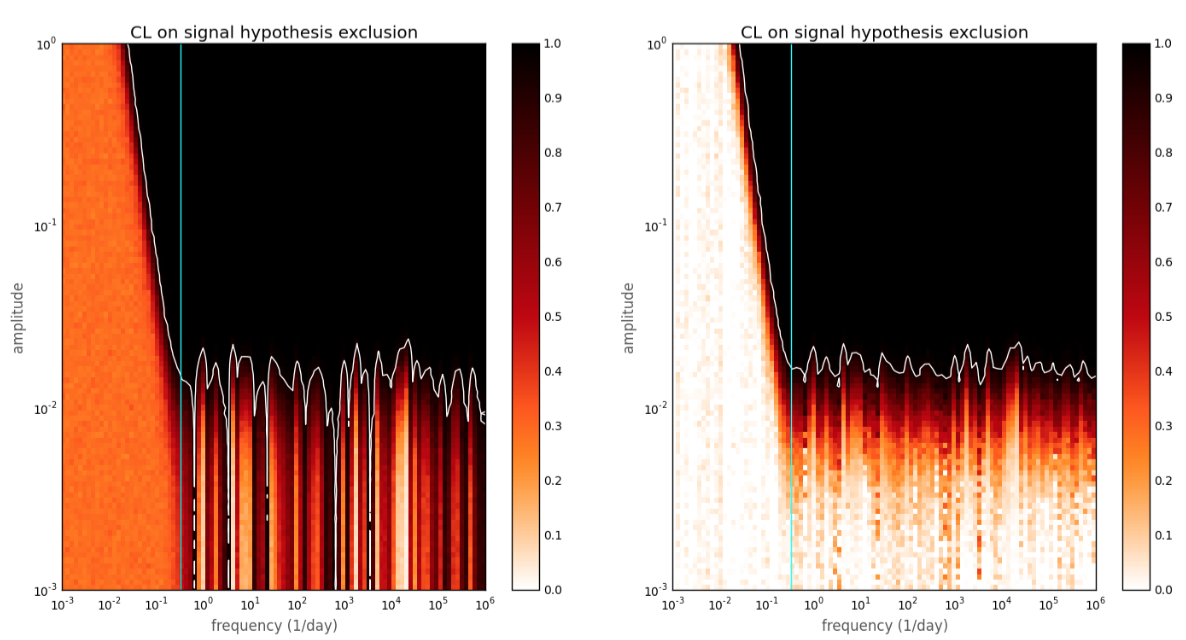
\includegraphics[width=\linewidth]{gfx/axions/exclusion_no_CLs.png}
  \caption{Confidence level \note{MR: need to establish whether we use CL or p-value} on rejection of various signal hypotheses, spanned by their amplitude and frequency. \emph{Left:} without the CLs method, \emph{right:} with the CLs method. The plots were produced with a test dataset, very different from the ILL dataset. The picture for the appropriate fake ILL dataset is in Fig.\,\ref{fig:ILL_exclusion}}.
  \label{fig:exclusion_no_CLs}
\end{figure*}

The result of this procedure applied to a fake ILL dataset is presented on the left--hand side in Fig.\,\ref{fig:ILL_exclusion}. Looking at the exclusion region, one sees that the sensitivity to exclude drops for both high and low frequencies. This can be understood by looking at Fig.\,\ref{fig:sensitivity}, where the power obtained in the Monte Carlo generation for various hypotheses is plotted on top of the signal periodogram. For hypotheses with the same assumed amplitude of oscillation, the amplitude seen in the periodogram is constant for periods between the separation of the data points and the total length of the data set. Longer periods are harder to exclude, as it is always possible that one is near an antinode of an extremely slow oscillation. This manifests itself as a high amplitude seen even when the null hypothesis is assumed. High frequencies are suppressed because the experiment measures the average of the oscillation over a run. There little amplitude is visible, despite assuming an oscillation of a large amplitude. In particular there are dips at the approximate sampling frequency (the data have not been taken perfectly regularly) and its multiples.

\begin{figure}[htb]
  \centering 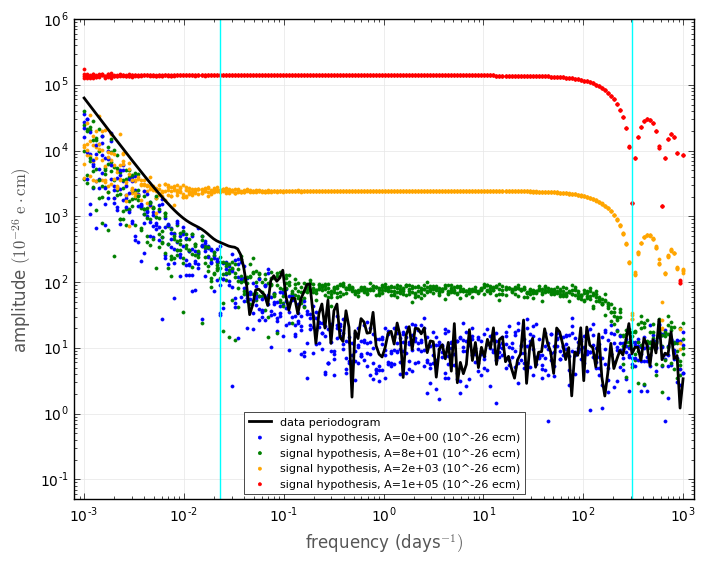
\includegraphics[width=\linewidth]{gfx/axions/sensitivity.png}
  \caption{For each frequency $f$, $\sqrt{\text{power}}$ is plotted for the dataset (black line) and MC--generated signal hypothesis of frequency $f$ and various amplitudes (different colours). For both high and low frequencies, the MC results approach the null hypothesis (blue). Also, a dip in power is nicely visible for oscillations coherent with the sampling frequency (and its multiples). The vertical lines depict the time--span of the dataset and the median separation between centres of runs.  The plot was produced with a test dataset, very different from the ILL dataset. \note{MR: It would be good for the sake of consistency to produce such a figure for the ILL fake dataset. - see fig \ref{fig:ILL_sensitivity}}}
  \label{fig:sensitivity}
\end{figure}

\begin{figure}[htb]
  \centering 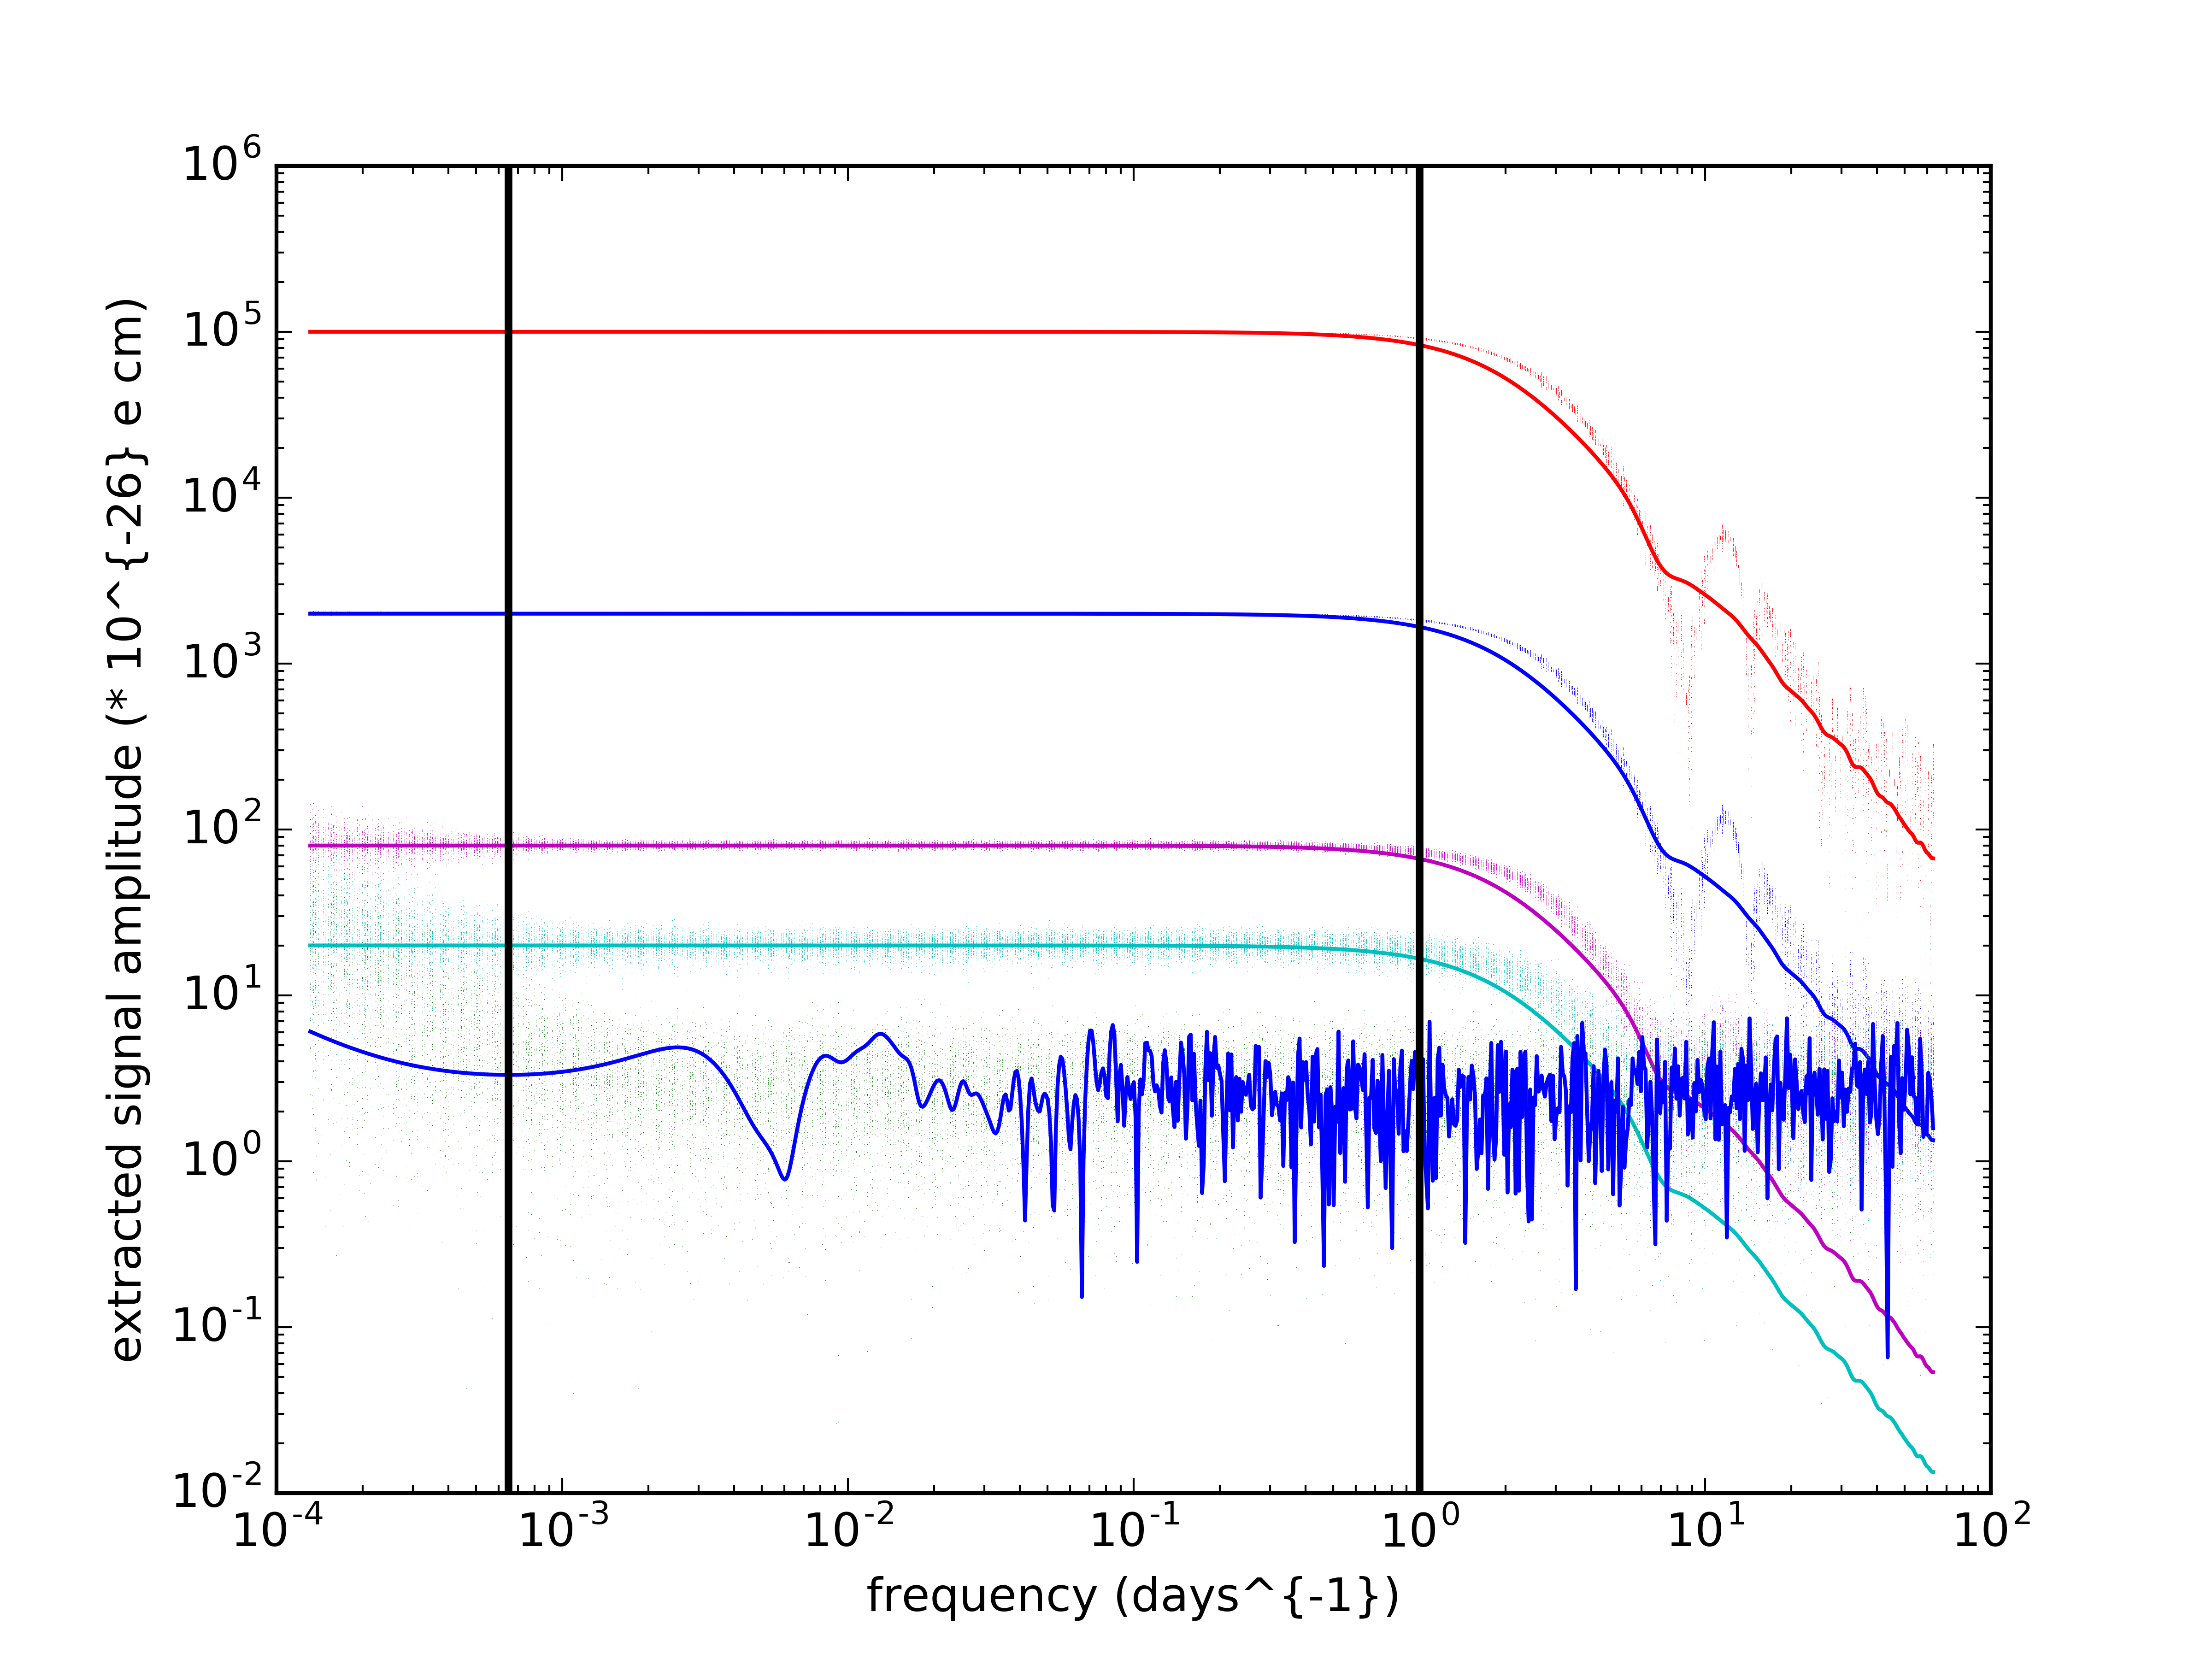
\includegraphics[width=\linewidth]{gfx/axions/ILL_signal_response_plot.png}
  \caption{The same plot as figure \ref{fig:sensitivity} for the ILL dataset}
  \label{fig:ILL_sensitivity}
\end{figure}


The 95\%~C.L. exclusion region, depicted by a white line on the left--hand side in Fig.\,\ref{fig:exclusion_no_CLs}, exhibits a number of thin peaks going down in very low amplitudes. Seemingly, for some frequencies, signals with amplitude far below the sensitivity of the experiment are excluded. This is disturbing. Consider, however, that as the power was evaluated for many frequencies, inevitably at some of them, roughly 5\%, the power is low enough to be rejected at 95\%~C.L. even when tested against the null hypothesis. However completely fine from the statistical point of view, physicists do not accept a situation, where a hypothesis is rejected based on an experiment which was not sensitive to it. One possible solution is called the \emph{CLs method}. The method is defined, as well as the problem itself discussed, in the booklet of the Particle Data Group~\citep{PDG2014}. Here we only shortly present its idea graphically in Fig.\,\ref{fig:CLs}. With use of the \emph{CLs method} exclusion is suppressed in the region of low sensitivity, as shown on the right--hand side in Fig.\,\ref{fig:exclusion_no_CLs}.

\begin{figure}[htb]
  \centering 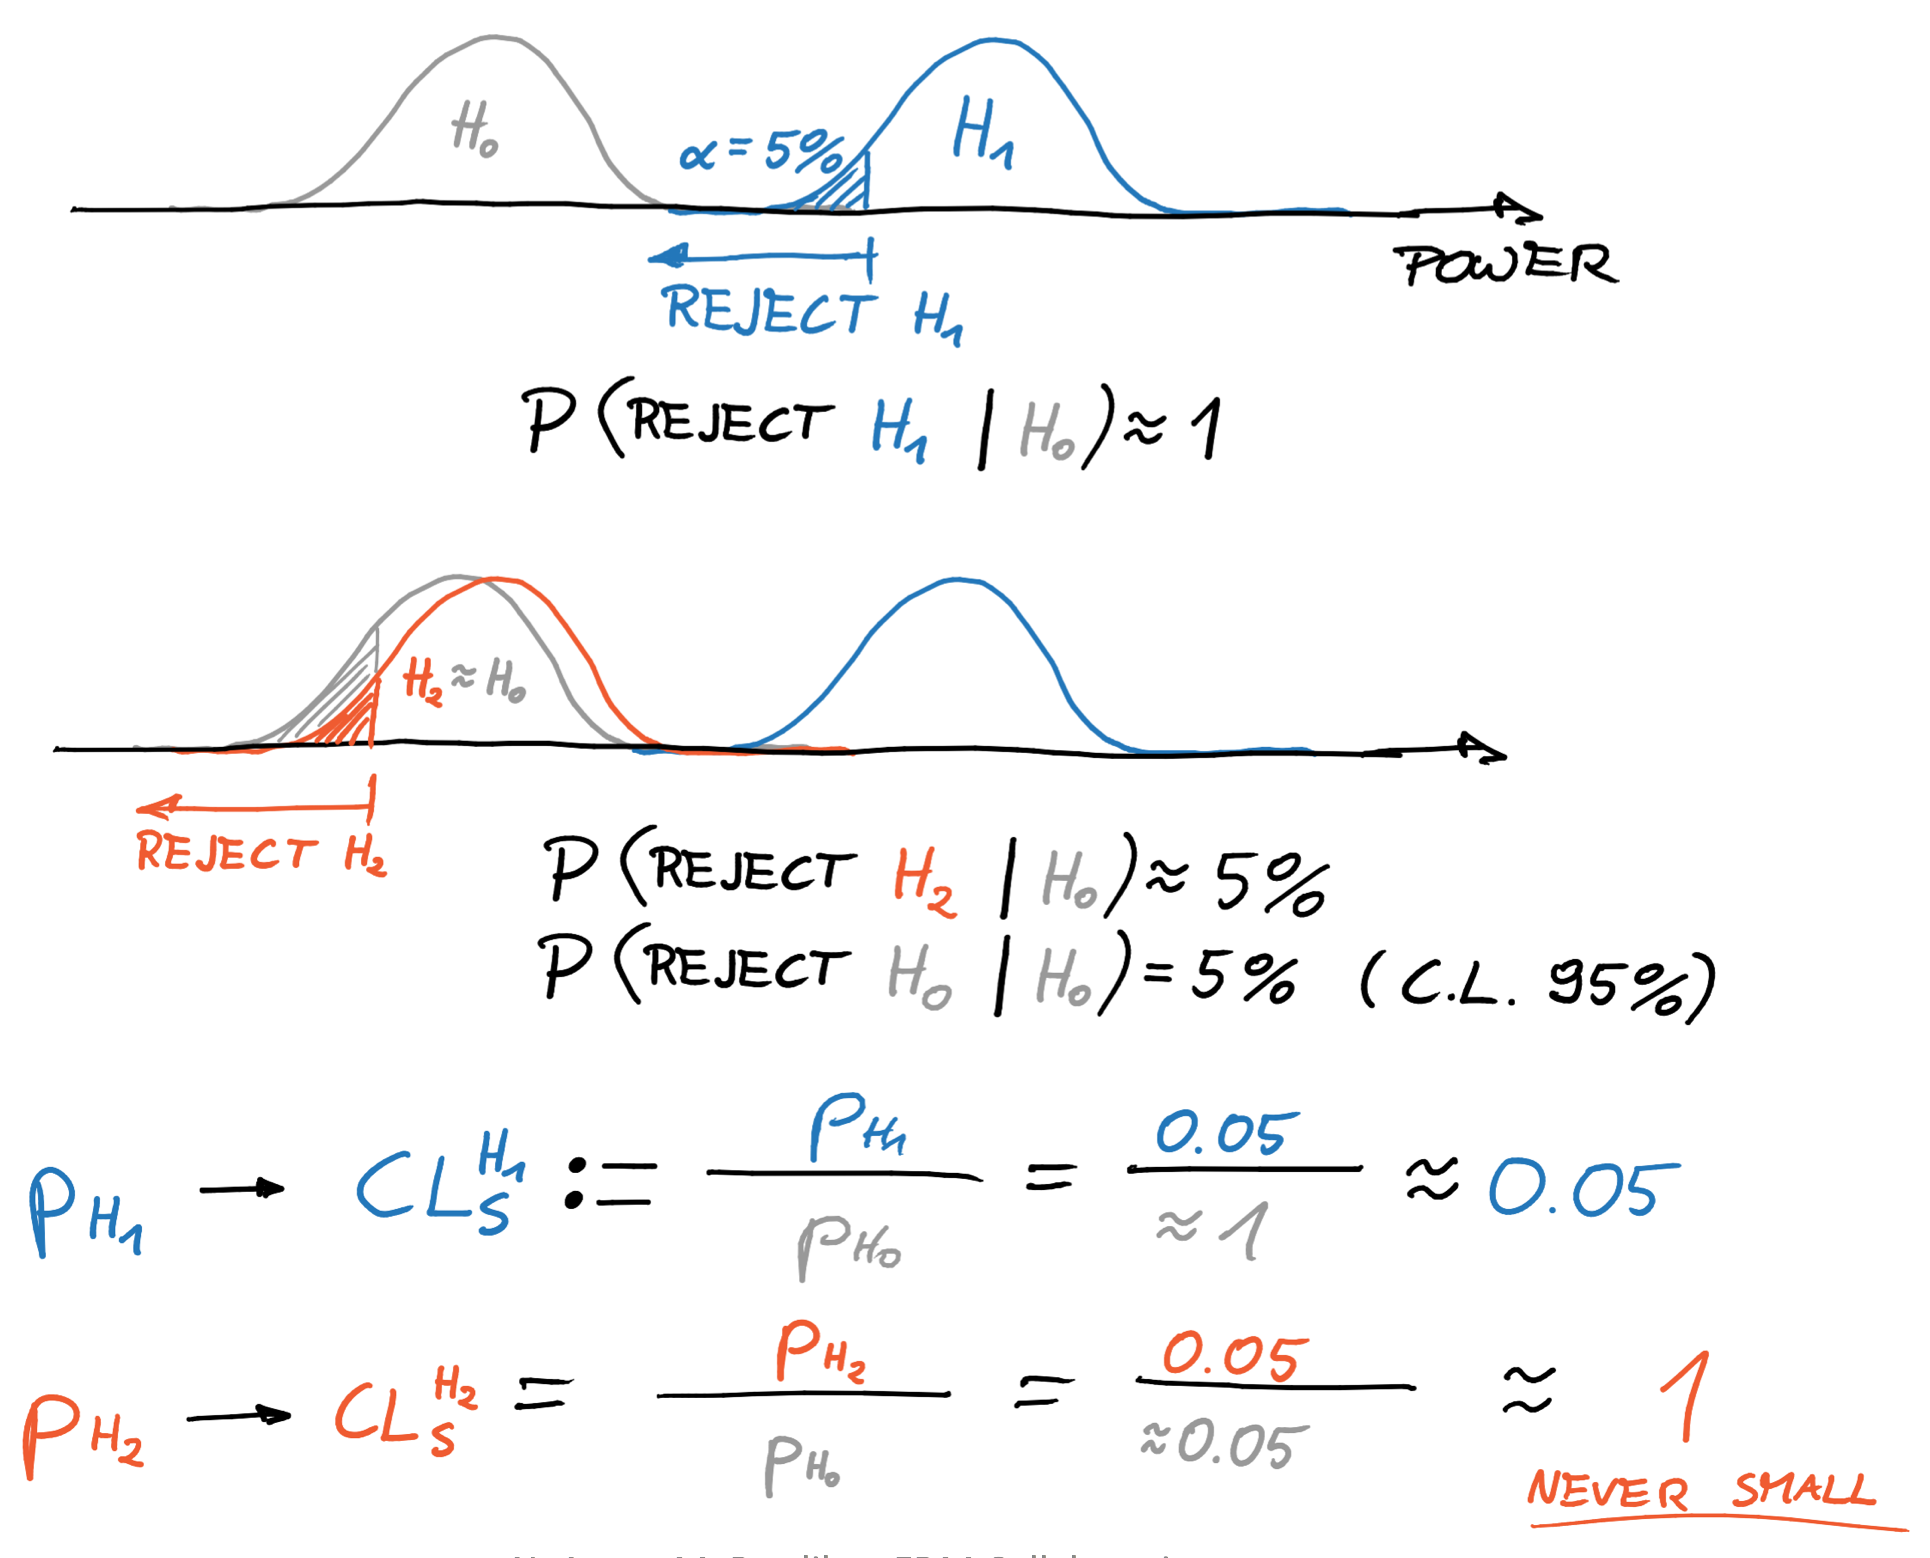
\includegraphics[width=\linewidth]{gfx/axions/CLs.png}
  \caption{The CLs method effectively suppresses power of hypotheses rejection if they are close to the null hypothesis.}
  \label{fig:CLs}
\end{figure}

Calculating each pixel of the alternative hypotheses space is largely a waste of resources. We are interested only in resolving the 95\% C.L. threshold. As a means of optimisation, we find the 95\% C.L. point for each frequency using the bisection algorithm. In only 10 steps it gives us relative precision below $0.01$ on its position. Thereby the final exclusion region is obtained \note{MR: figure needed, with the line only. It is missing for now for the run--level, but is present for the cycle--level}.


\subsection{Run--level Systematic Effects Discussion}
\note{To be filled by NA}. An analysis without a constant offset in the LSSA fit is possible if all known systematic effects that would cause a shift in the $d_n$ level are taken into account. In case of the ILL experiment, these have already been thoroughly studied for the mainstream nEDM analysis. A detailed reanalysis of all known systematic effects gave an overall systematic uncertainty of $\unit[0.38 \pm 0.99 \cdot 10^{-26}]{e\cdot cm}$ \cite{Pendlebury2015}. The central value was subtracted from the entire dataset, and the uncertainty on this value was considered small enough to be safely ignored, being around a tenth of the size of the oscillations we are sensitive to. This improves the sensitivity of the analysis to slow oscillations. \note{MR: We need to be absolutely sure that the exotic physics would NOT cause a shift, but only an oscillation around zero.} \note{YS: We are assuming that the only effects of exotic physics are due to the oscillating EDM here (with no extra static EDM), see footnote [39].}

The largest systematic effect in the ILL experiment

\note{MR: When we do that for the run--level analysis, we need to state the reason why is it not done for the cycle--level analysis. Possible reasons:
\begin{enumerate}
  \item Systematic studies are not yet finished.
  \item Maybe there is a reason why it is not at all possible. In run--level some systematic effects cancel when we bring the two field configurations (parallel and anti--parallel) together. In cycle--level they are considered separately.
\end{enumerate}
}

\note{MR: Another, more compact version of the run--level analysis description. \textbf{OUTDATED BY NOW}

  \subsection{Run--Level (ILL data) Least Squares Spectral Analysis}
  We are looking for oscillations by applying least--squares spectral analysis (LSSA) \note{MR: citation needed} to a time series of $d_n$ extracted from each run. Thereby a linear fit to the time series is performed with model:
  \begin{equation}
  	A\,\mathrm{cos}(\omega t) + B\,\mathrm{sin}(\omega t) + C
  \end{equation}
  Power at frequency $\omega$ is defined as $P(\omega) := A^2 + B^2$. We analyse a fixed set of 200 frequencies $\omega_i$ (although this number may increase in the future).

  In order to test the resultant periodogram against the null hypothesis, PDF of the latter is generated with Monte Carlo for each frequency $\omega_i$, assuming that points of the $d_n$ time series come from a normal distribution with width equal to the error--bars. Taking into account the look---elsewhere effect, false--alarm threshold at $\omega_i$ is set at $n$th \note{MR: need a number here} percentile of the obtained PDF \note{MR: cite solar neutrinos here}. The results are shown in Fig.\,\ref{fig:ILL_detection}.

  % \begin{figure}[h!]
  % \begin{center}
  % \includegraphics[width=\columnwidth]{ILL}
  % \caption{TODO}
  % \label{fig:ILL_detection}
  % \end{center}
  % \end{figure}

  In order to obtain the exclusion region we test many alternative hypotheses $H_s$. In each we assume a perfectly coherent signal of frequency $\omega_s$ (the axion field has coherence time of $\approx 10^6$ periods \note{MR: I think it belongs here, as here it really matters}), amplitude $A_s$ and random phase. We generate many time--series, taking for each point the model averaged over the duration of the run \note{MR: To be \textbf{really} proper we would average over the free precessions of the run. We don't do it because we're lazy (and it doesn't matter) or is the timing information not available? PH: The accuracy of the timing information was limited, since the DAQ computer relied on its internal clock - there was no comparison with external atomic clocks, and there could easily be drifts of seconds to minutes.  For shorter timescales, therefore, the PSI data are far superior.}. From the time--series we evaluate PDF of $P(\omega_s)$. We do a one--side test looking for unlikely small amount of power in the data periodogram.

  Additionally we employ the CLs method \note{MR: citation needed} to dampen exclusions in the insensitive region. Thereby the p--value of the alternative hypothesis test $p_s$ is normalised to the p--value of corresponding test of the null hypothesis $p_0$. We consider the hypothesis as excluded when $p_s / p_0 < 0.05$. Results are in Fig.\,\ref{fig:ILL_exclusion}.

  % \begin{figure}[htb]
  % \begin{center}
  % \includegraphics[width=\columnwidth]{ILL_exclusion}
  % \caption{TODO \note{MR: I would present this figure like this: light, pastel colours for the run--level with a thick line at p-value = 0.05. The cycle--level analysis I would put on the same figure, but only the thick line.}}
  % \label{fig:ILL_exclusion}
  % \end{center}
  % \end{figure}
}


\section{Short time--base analysis}
\subsection{The PSI nEDM experiment}
The Sussex--RAL--ILL apparatus was moved to PSI where, benefiting from a stronger UCN source, and upon numerous improvements continues to measure the nEDM with ever increasing precision.

The most important thing for this analysis upgrade is the deployment of a Cesium magnetometer array \note{MR: citation needed} around the precession chamber. They allow for continuous measurement of the vertical magnetic field gradient $\partial_z B_z$ and thus correcting for drifts of the vertical magnetic field gradient on a cycle--basis, as in \ref{eq:R}.

Also, the PSI experiment is timed with GPS--referenced clocks. Precise timing allows for performing the analysis at higher frequencies reliably. \note{MR: Do we need that really? Maybe not mention it.}

\subsection{Differences to the long time--base analysis}
Going to a cycle--level analysis presents new challenges. The $d_n$ value cannot be extracted on cycle--basis. The spectral analysis is performed on $R := \frac{f_n}{f_{\mathrm{Hg}}}$ instead, which already includes $^{199}\mathrm{Hg}$ comagnetometer's correction for magnetic field drifts. The axion signal would appear there as an oscillation of amplitude dependent on the electric and magnetic field configuration: $0$ for $E=0$, $\pm \ \frac{h\, \gamma_{Hg} \langle B_0 \rangle }{2 E}$ for the parallel and anti--parallel configuration of $\vec{E}$ and $\vec{B}$, respectively (see Figure\,\ref{fig:cycle-level_phase_flip}). \note{note: relative fluctuations of $B_0$ are on the level of $10^{-6}$}. These three datasets are analysed separately --- the two $E \neq 0$ datasets are sensitive to an axion particle, while $E=0$ is a control data set.

\begin{figure}[htb]
  \centering 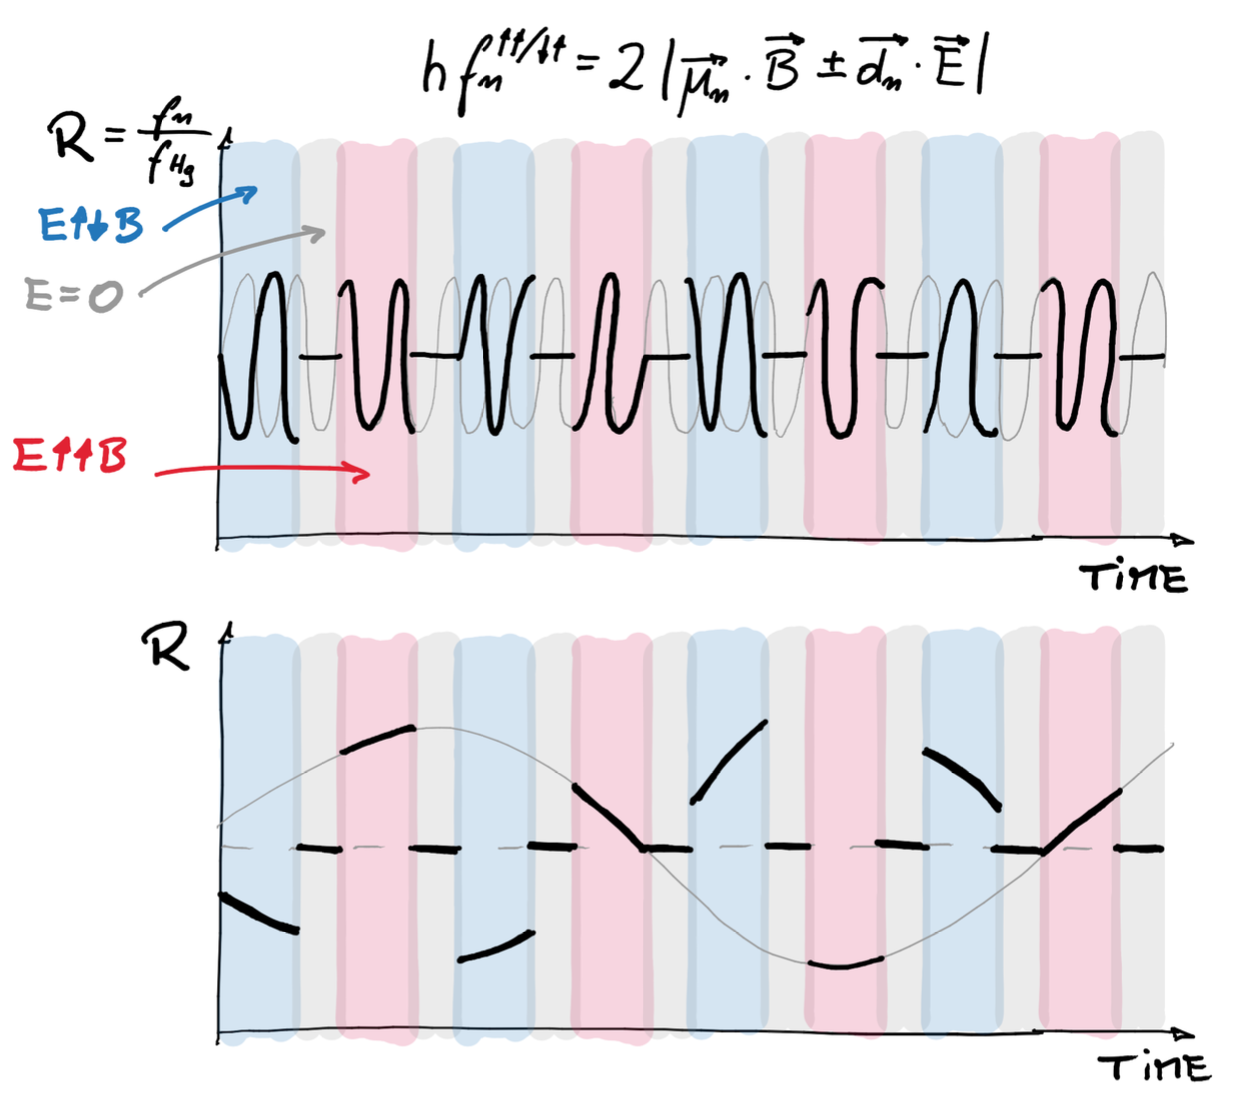
\includegraphics[width=\linewidth]{gfx/axions/cycle-level_phase_flip.png}
  \caption{A sketch of how an axion--induced signal would appear in the $R$ time--series.}
  \label{fig:cycle-level_phase_flip}
\end{figure}

The presence of a magnetic field gradient $\frac{\partial B_z}{\partial z}$ causes a shift in $R$ (see Eq.\,(\ref{eq:R})). While the constant component of the shift is rejected by the spectral analysis, the Cesium magnetometer array \note{MR: citation needed} is used to correct for drifts of the gradient. The standard measurement procedure of the PSI nEDM experiment involves deliberate setting of a vertical gradient and changing it from run to run, as shown in Fig.\,\ref{fig:cycle-level_gradient_jump}. Additionally, the Caesium magnetometers are calibrated after each change, which alters systematic offsets in their readout. For these reasons correction for the magnetic field gradient across different runs is potentially unreliable and has not been done. Instead, the offset parameter $C$ in the LSSA fit is allowed to be different in each run. Sensitivity in periods larger then one run is thus sacrificed, but in this region the run--level analysis delivers a better limit. Last, but not least, the majority of the PSI data is blinded \note{MR: citation needed} --- an unknown constant $d_n$ has been injected into the data. As the data are not going to be unblinded for this analysis only, we cannot assume zero constant $d_n$. This makes combining the datasets hard, as the axion--induced oscillation would not be centered around the $R$ value measured without the electric field, as sketched in Fig.\,\ref{fig:cycle-level_blinding_offset}. Performing the analysis separately on the three datasets with different field configurations: $E=0$, $E \uparrow \uparrow B$ and $E \uparrow \downarrow B$, combined with allowing for different offsets $C$ in each run, greatly simplifies the analysis.

\begin{figure}[htb]
  \centering 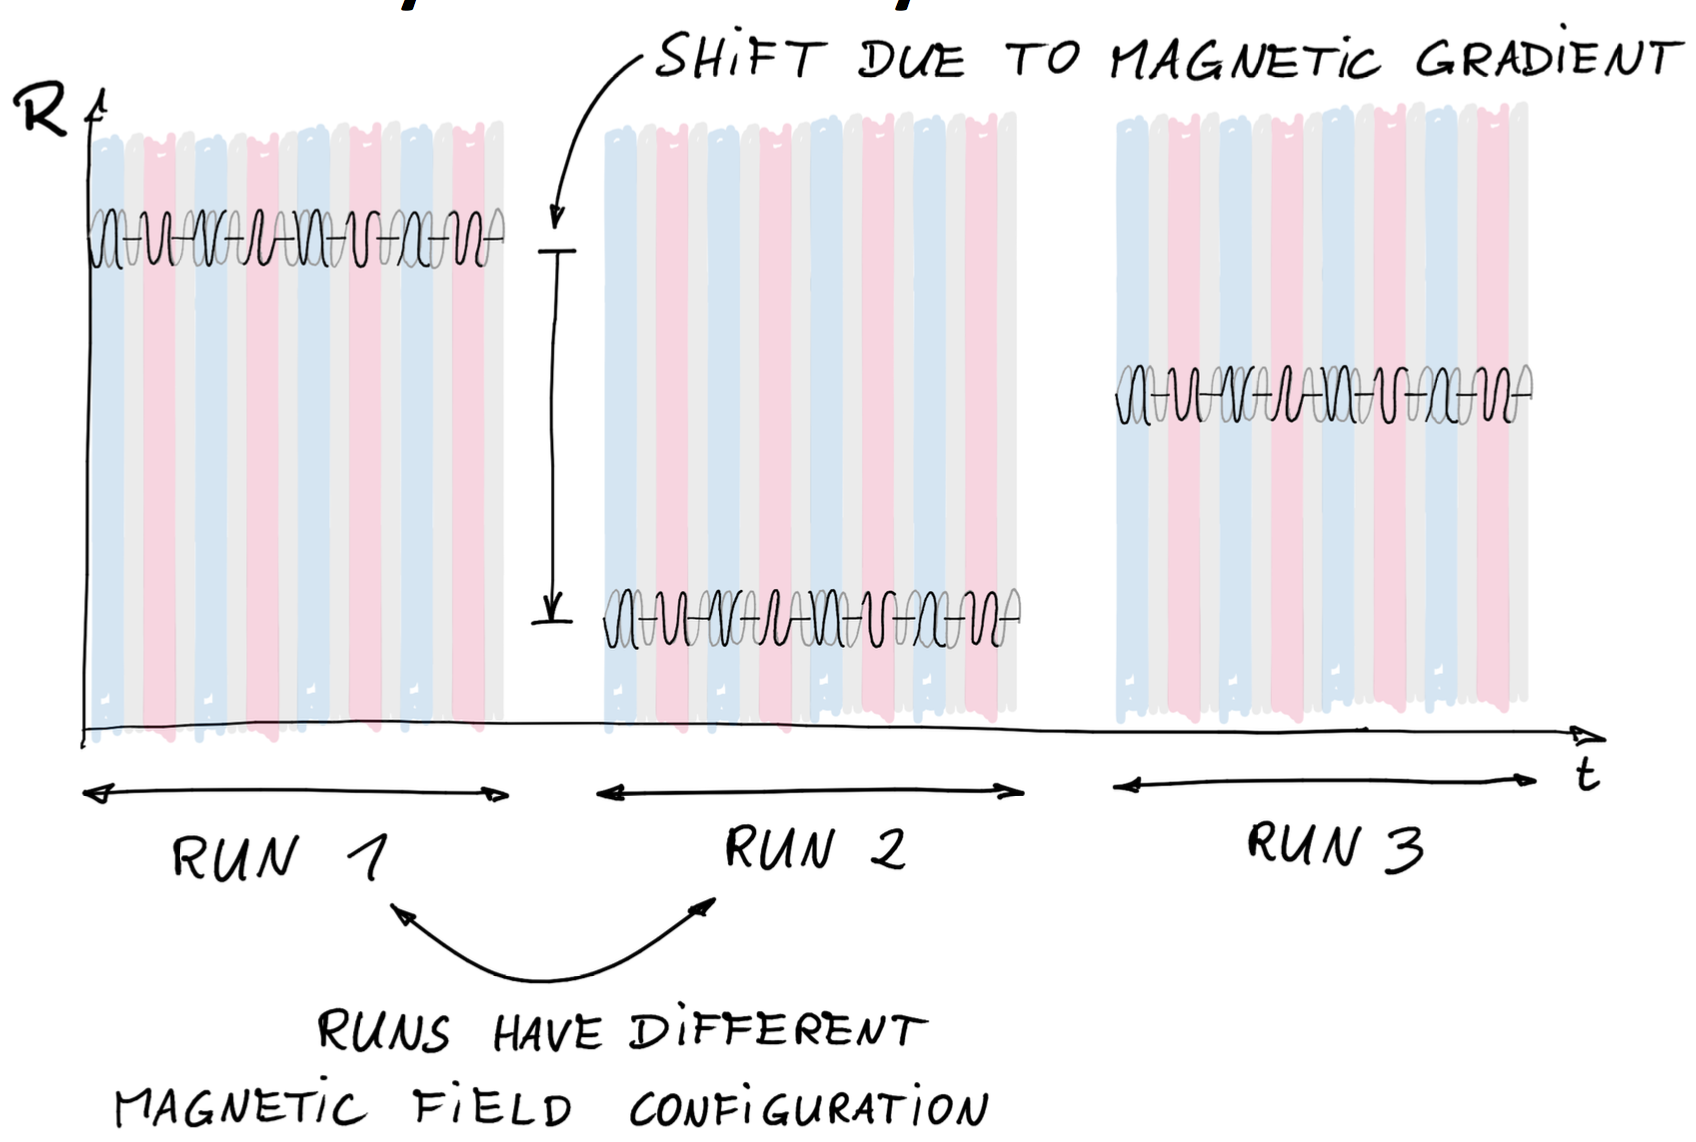
\includegraphics[width=\linewidth]{gfx/axions/cycle-level_gradient_jump.png}
  \caption{A sketch of how the $R$ time--series with an axion signal would look like across different runs.}
  \label{fig:cycle-level_gradient_jump}
\end{figure}

\begin{figure}[htb]
  \centering 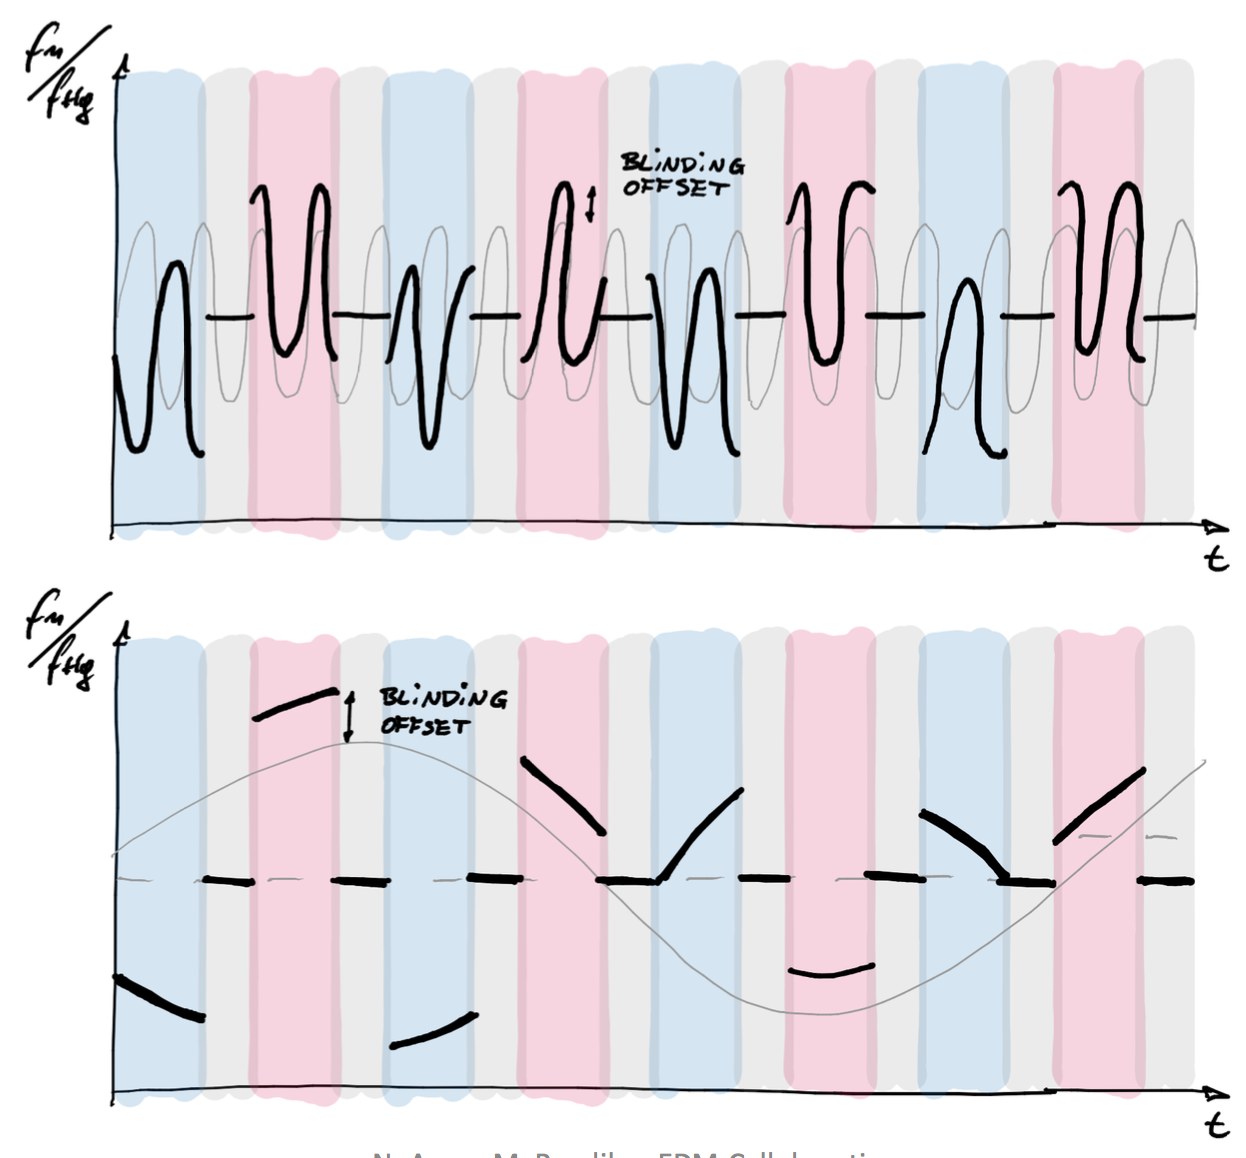
\includegraphics[width=\linewidth]{gfx/axions/cycle-level_blinding_offset.png}
  \caption{A sketch of how the blinding offset, and the true $d_n$, affect the $R$ time--series with a hypothetical axion--induced oscillation.}
  \label{fig:cycle-level_blinding_offset}
\end{figure}

The neutrons accumulate the phase during the free precession period. Therefore, the precession frequency that is measured is averaged over this period. In the Monte Carlo simulations it is assumed that the averaging occurs between the centres of the $\unit[2]{s}$ long spin--flip pulses, which is $\unit[202]{s}$.

\note{MR: How to combine the two data--sets? Gain in sensitivity only minor when using both. Maybe one can adjust for each hypothesis CL. 95\% -> $1 - \sqrt{0.05} = 0.78$, then something not seen in both on CL 78\% is exculded at 95\%. Would be tricky to implement exactly (the exclusion regions from the two datasets are not \emph{exactly} the same). What to do with the E=0 data--set? Cannot correct with it (checked that). Maybe just leave it as a check.}

The PSI data set uses, naturally, a different set of frequencies then the RAL--Sussex one. Due to the shorter time of data taking, the spectral resolution is lower (the inverse of $4.5$ months, $\unit[\sim 10^{-9}]{Hz}$), but denser sampling allows for going to higher frequencies. For the highest frequency we choose $\approx \unit[4 \cdot 10^{-3}]{Hz}$ \note{MR: still to be discussed}, which is a bit larger than the inverse separation of cycles. Then we choose the complete set of frequencies in an analogous way to the long time--base analysis, arriving at $\sim 10^6$ frequencies to analyse.

% \begin{figure}[htb]
% \begin{center}
% 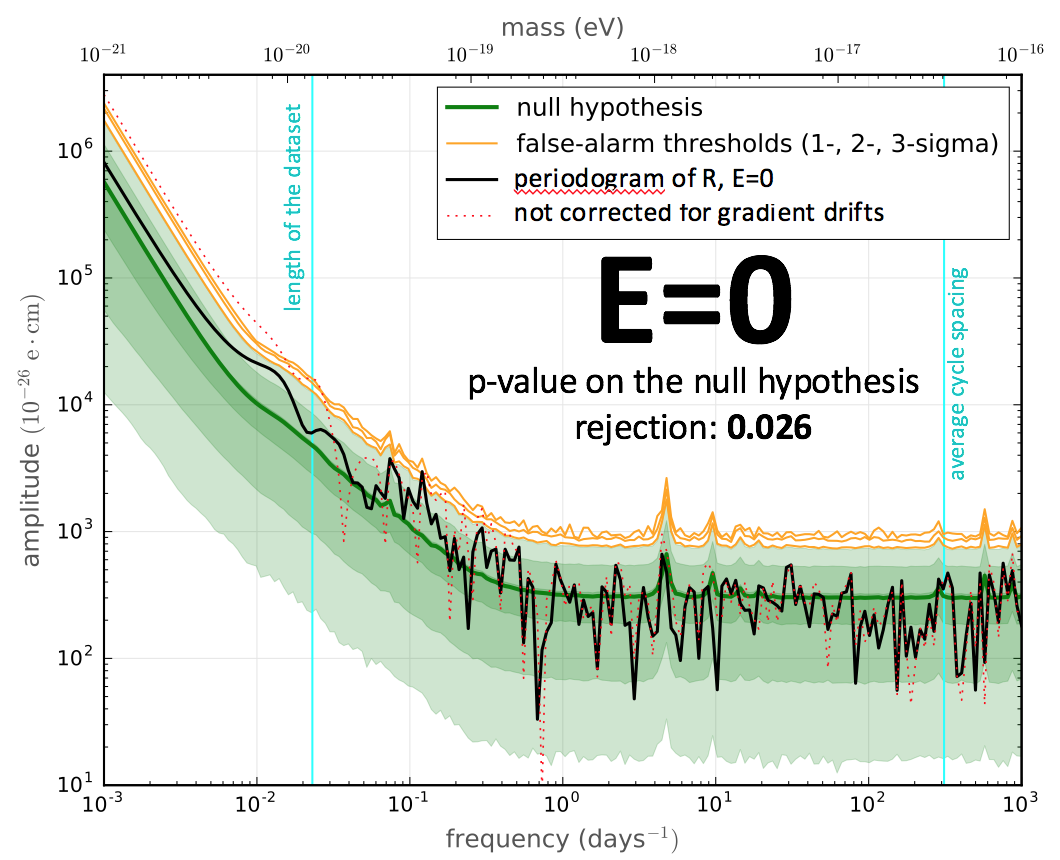
\includegraphics[width=0.5\columnwidth]{PSI_E0}
% 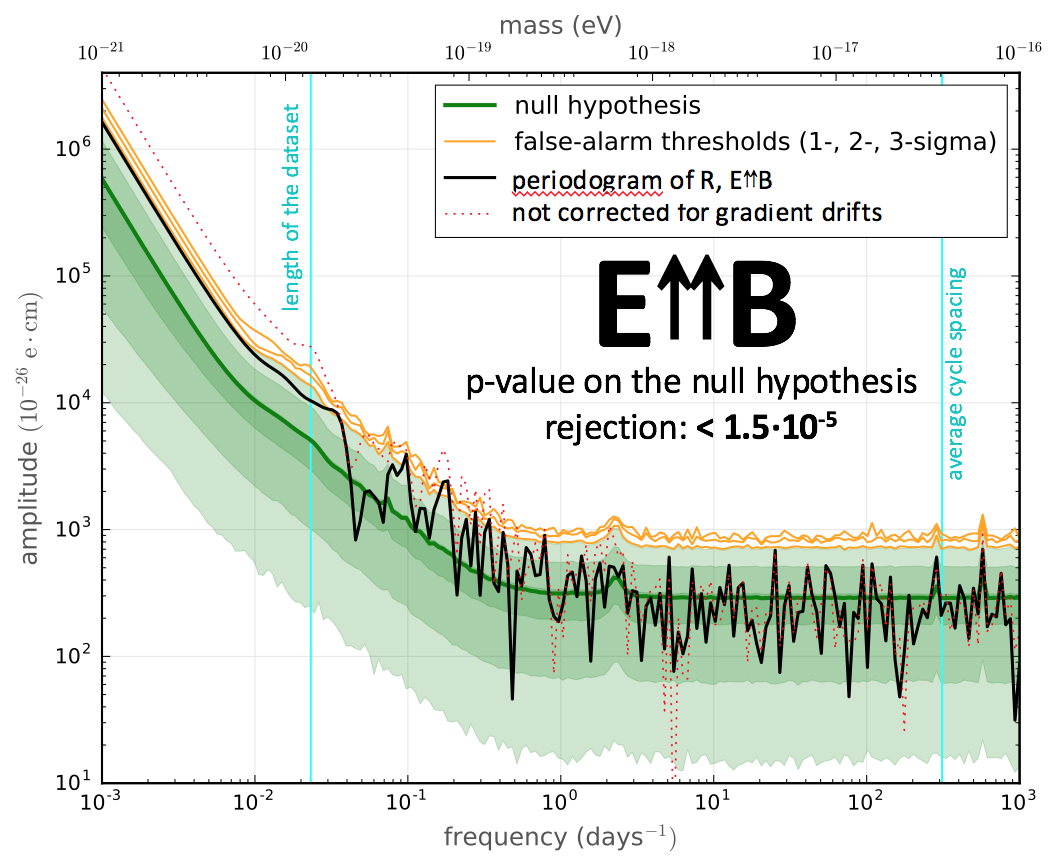
\includegraphics[width=0.5\columnwidth]{PSI_EpB}
% 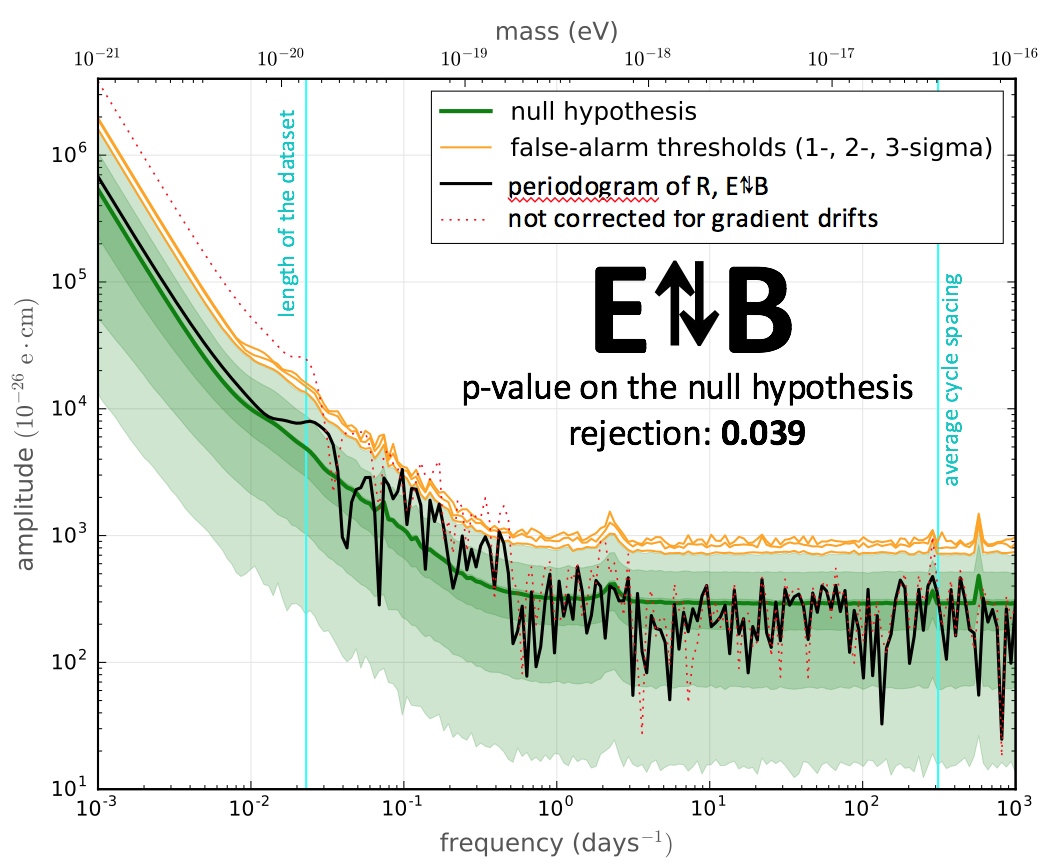
\includegraphics[width=0.5\columnwidth]{PSI_EapB}
% \caption{TODO \note{MR: The null hypothesis band is nearly identical for $E \neq 0$. Maybe plot only one and on top of that two periodograms of data? Also the plot is quite cluttered. Maybe plot only 95th percentile green line and 5\% false alarm threshold. Do NOT plot the bottom of distribution band -- it is meaningless, at least for our needs.}}
% \end{center}
% \end{figure}


\subsection{Systematic Studies for the Cycle--Level Analysis}
While the run--level analysis can benefit from all of the systematic studies done for the constant nEDM measurement, this is not the case for the lower level cycle--level analysis. An important decision has to be taken on how to treat the systematic effects. There are three options:
% \begin{enumerate}
%   \item Perform a detailed study of time--dependent systematic effect.
%   \item Determine \emph{delicate} frequencies and cut them out.
%   \item Assume there are no systematic effects.
% \end{enumerate}

\paragraph{Perform a detail study of time--dependent systematic effect.}
Here we would assume that any excess in power, in any dataset ($E \uparrow \uparrow B$, $E \uparrow \downarrow B$ and $E=0$) is a signature of some kind of a signal. All effects that can potentially result in that should be identified before the analysis is performed and corrected for. This would require a long and careful systematic study, a task much bigger then this analysis itself. Moreover, the full--fledged systematic studies for the constant nEDM analysis of the PSI data are still ongoing. Even though we acknowledge that this would be \emph{the} proper way to go, we consider it to be unrealistic and unnecessary for this analysis.

\paragraph{Determine \emph{delicate} frequencies and cut them out.}
Looking at periodograms of raw data one sees that there are several typical frequencies where peaks appear. Typically at inverse specific time constants at which the experiment operates: cycle separation, day, week, , HV--reversal, B0--reversal. We may decide that all systematic effects are constrained to these frequencies and do not perform the analysis there at all.

\paragraph{Assume there are no systematic effects.}
An axion would produce a very specific signal, in particular:
\begin{enumerate}
  \item There would be no signal in the $E=0$ dataset.
  \item The signal would appear in both $E~\uparrow~\uparrow~B$ and $E~\uparrow~\downarrow~B$ datasets, with equal amplitude.
  \item The signals in $E \uparrow \uparrow B$ and $E \uparrow \downarrow B$ would be shifted in phase by 180~degrees.
  \item The signals would have to have a high coherence of $\delta f / f = 10^{-6}$.
\end{enumerate}
In case we see an excess in power, we would only call it a candidate for an axion--signal if the three above conditions are met. Otherwise we attribute it to a, potentially unknown, systematic effect. We do realise the danger of making the systematic search dependent of the act of finding a signal. This automatically opens a line of attack on this analysis: we would not make a discovery, because a systematic effect has canceled the real signal out. We would not have seen a signal and therefore not looked for systematic effects. This is certainly valid. Nevertheless, we argue that the extremely low probability of this event, due to the high coherence of the axion field, makes it negligible. In order to cancel the axion signal, a systematic effect would not only need to be as coherent as the axion field, but additionally fine--tuned over at least 5 orders of magnitude magnitude of tested frequencies. With the coherence of $\delta f / f = 10^{-6}$ this is a tuning of $10^{-30}$. It would also need to be fine--tuned in amplitude over $\sim 20$ orders of magnitude, which gives a rough estimate of the cancellation probability: $10^{-50}$. As we are presenting limits with 95\% C.L., we feel this approach is justified.

Out of the three, we opt for the third option, but leave the subject open to discussion for the collaboration.


\subsection{Results of the short time--base analysis}
At the moment only a $\approx 40$ days long subset of the PSI data set has been analysed. The full data set will be analysed when the analysis method has been exactly established.

The results of the null hypothesis tests are presented in Fig.\,\ref{fig:cycle-level_detection}. Even though the data taking is not strictly synchronous throughout the whole data taking period, it is highly regular. This causes structures visible in the distributions of the null hypothesis periodograms. There is a sharp peak at the inverse median of the data points (cycles of the experiment), equal to $\unit[301]{s}$. The broader peaks at approximately inverse 10~hours in $E \neq 0$ and 5~hours in $E = 0$ datasets correspond to the periodicity of electric field changes in the apparatus. The electric field is changed according to the pattern: 8 cycles of no field, 48 in one direction, 8 of zero, 48 in the other direction. Thanks to the Monte Carlo simulations, the structures in the periodograms are reproduced and accounted for in the hypotheses testing.

The global p-values for the $E=0$ and $E \uparrow \downarrow B$ are 0.53 and 0.12 respectively, indicating agreement with the null hypothesis. The global p-value for the $E \uparrow \uparrow B$ dataset is $3.4 \cdot 10^{-5}$, which is on the 4--sigma level. However, the corresponding frequency is in the delicate region around the inverse median spacing of data points. As the peak does not appear in the $E \uparrow \downarrow B$ dataset, and the 5--sigma threshold has not been crossed, we do do not consider it to be an indication of an axion signal.


\begin{figure}[h!]
  \centering 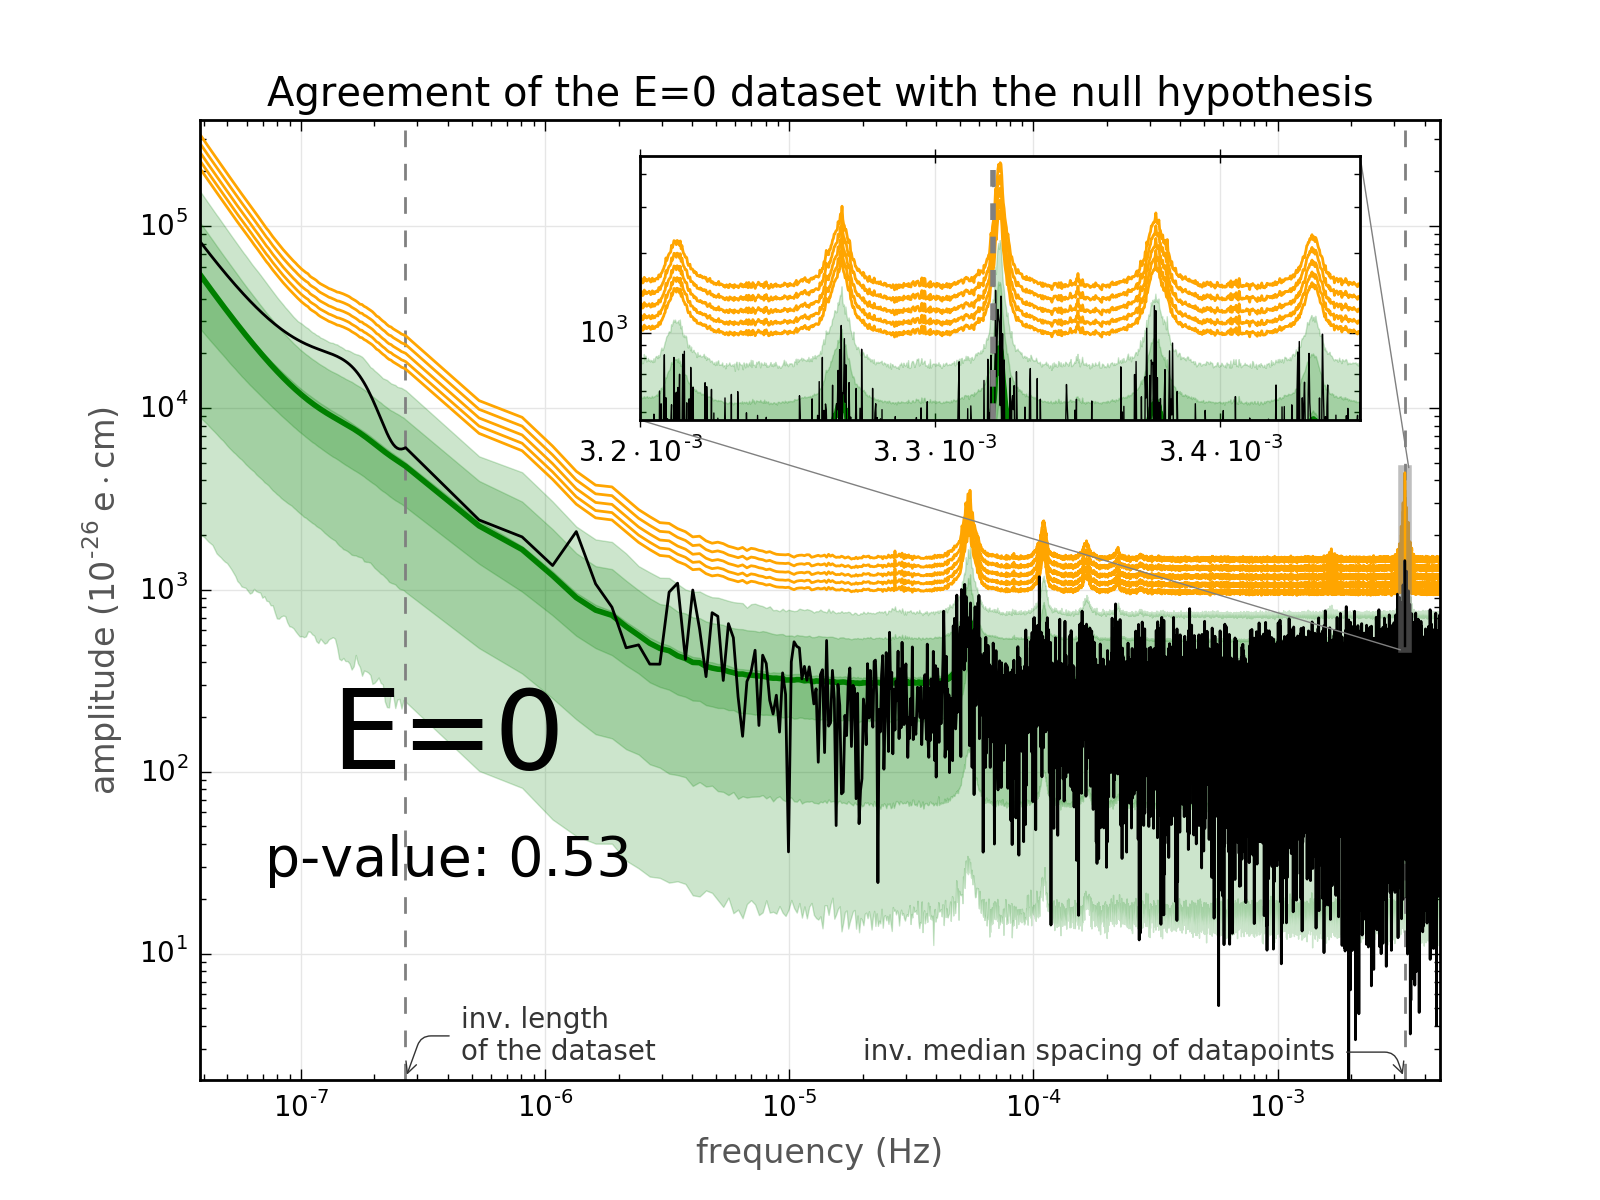
\includegraphics[width=0.9\linewidth]{gfx/axions/cycle-level_E0_detection.png}
  \centering \includegraphics[width=0.9\linewidth]{gfx/axions/cycle-level_EBp_detection.png}
  \centering \includegraphics[width=0.9\linewidth]{gfx/axions/cycle-level_EBap_detection.png}
  \label{fig:cycle-level_detection}
  \caption{Results of the three datasets ($E=0$, $E \uparrow \uparrow B$, $E \uparrow \downarrow B$) compatibility with the null hypothesis tests. The two--dimensional distribution of the null hypothesis periodogram is depicted with green bands, thick green line being the mean. The orange lines depict 1-, 2-, 3-, 4- and 5-sigma false--alarm thresholds. The inverse length of the dataset and inverse median spacing of the datapoints are marked with dashed vertical lines. The structures visible in the distribution of the null hypothesis periodogram are solely due to the time scheme of data taking. High correlation for frequencies lower then the inverse length of the dataset is visible even with bare eye. This is expected, as those frequencies are separated by less then the spectral resolution of the data set.}
\end{figure}

% \begin{figure}[htb]
%   \centering 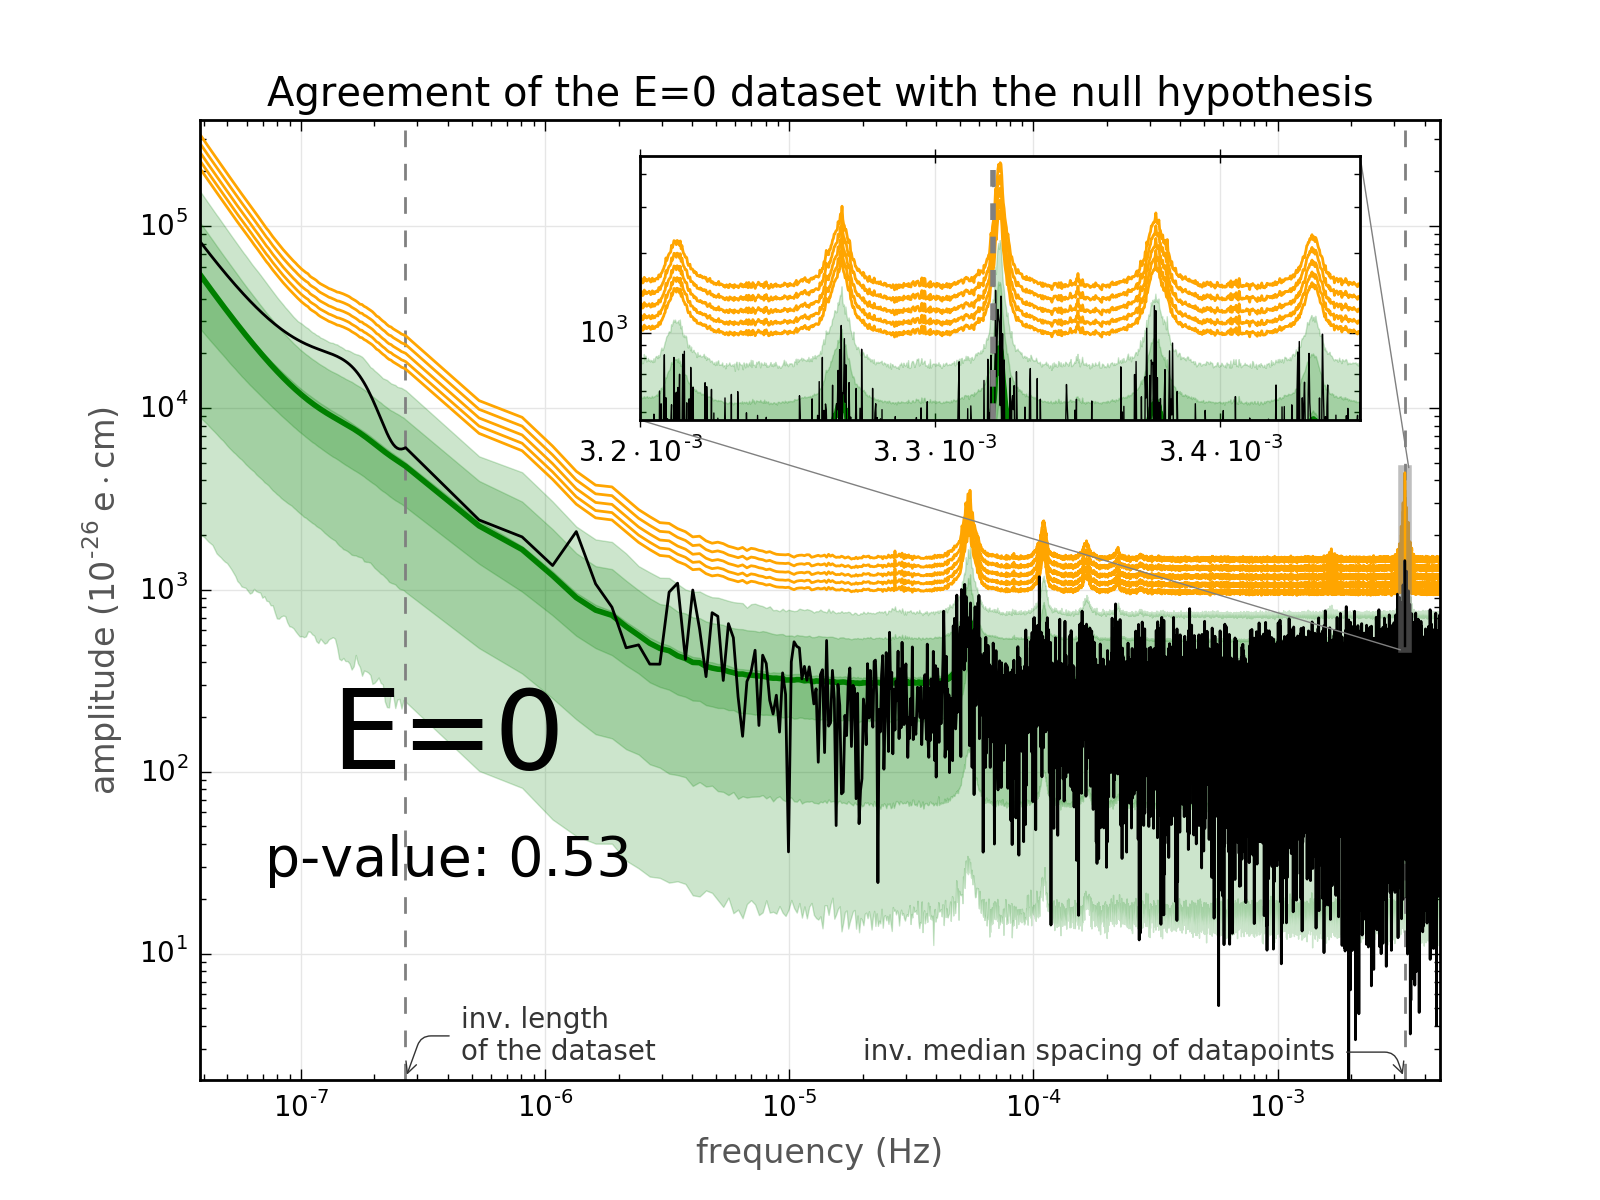
\includegraphics[width=\linewidth]{gfx/axions/cycle-level_E0_detection.png}
%   \caption{Results of the test dataset ($E=0$) compatibility with the null hypothesis. The two--dimensional distribution of the null hypothesis periodogram is depicted with green bands, thick green line being the mean. The orange lines depict 1-, 2-, 3-, 4- and 5-sigma false--alarm thresholds. The inverse of the length of the dataset and of the median spacing of the datapoints are marked with dashed vertical lines. The structures visible in the distribution of the null hypothesis periodogram are solely due to the time structure of how the data was taken.}
%   \label{fig:cycle-level_E0_detection}
% \end{figure}
%
% \begin{figure}[htb]
%   \centering \includegraphics[width=\linewidth]{gfx/cycle-level_EBp_detection.png}
%   \caption{\note{MR: TODO The very low p-value is due to a peak (on a 4--sigma level) which is very close to the inverse median spacing of datapoints. Need to investigate. Will it appear in EBap dataset too?}}
%   \label{fig:cycle-level_EBp_detection}
% \end{figure}
%
% \begin{figure}[htb]
%   \centering \includegraphics[width=\linewidth]{gfx/cycle-level_EBap_detection.png}
%   \caption{\note{MR: TODO}}
%   \label{fig:cycle-level_EBap_detection}
% \end{figure}

The exclusion regions obtained from the two $E \neq 0$ datasets are shown in Fig.\,\ref{fig:cycle-level_exclusion}.

\begin{figure}[htb]
  \centering 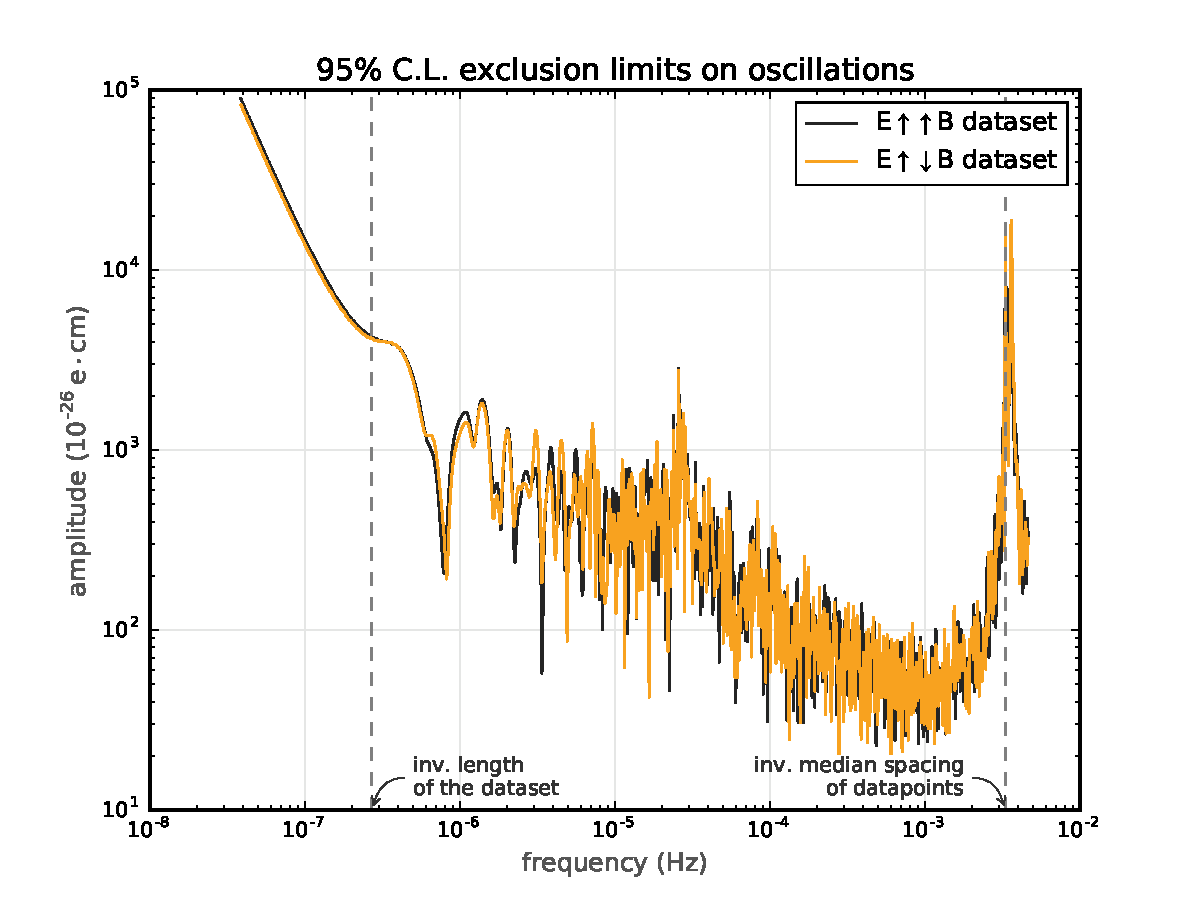
\includegraphics[width=\linewidth]{gfx/axions/cycle-level_exclusion_bisection.pdf}
  \caption{Exclusion regions obtained with the $E \uparrow \uparrow B$ and $E \uparrow \downarrow B$ datasets. Excluded are amplitudes higher then the line drawn. The regions for the two datasets are nearly identical, as expected. For periods longer then the length of the dataset a rapid loss of sensitivity is observed. Also, sensitivity to exclusion is significantly worse in the region around the inverse median spacing of the datapoints (equal to the cycling frequency of the experiment).}
  \label{fig:cycle-level_exclusion}
\end{figure}



%%%%%%%%%%
\section{Results in the axion context}


\note{Present results (including graphs) for axion-gluon coupling, and $g_d$ effective coupling (to compare with CASPEr notation)?, axion-neutron coupling, axion-proton coupling, axion-electron coupling?}






%%%%%%%%%%
\textbf{Conclusions.} ---
















%%%%%%%%
%\section*{ACKNOWLEDGEMENTS}
\textbf{Acknowledgements.} ---
\note{We are grateful to Maxim Pospelov and Edward Witten for helpful discussions. This work was supported by .... }

%the Australian Research Council.
%the Royal Astronomical Society.



%%%%%%%%%
%\section*{Appendix}
\appendix

%%%%%%%%%%
\textbf{Appendix A:~Summary of Existing Constraints.} ---
Here we summarise the existing constraints on the axion mass and interaction parameters in Eq.~(\ref{Axion_couplings}) from laboratory searches and measurements pertaining to astrophysics and cosmology.

\begin{figure}[h!]
  \begin{center}
  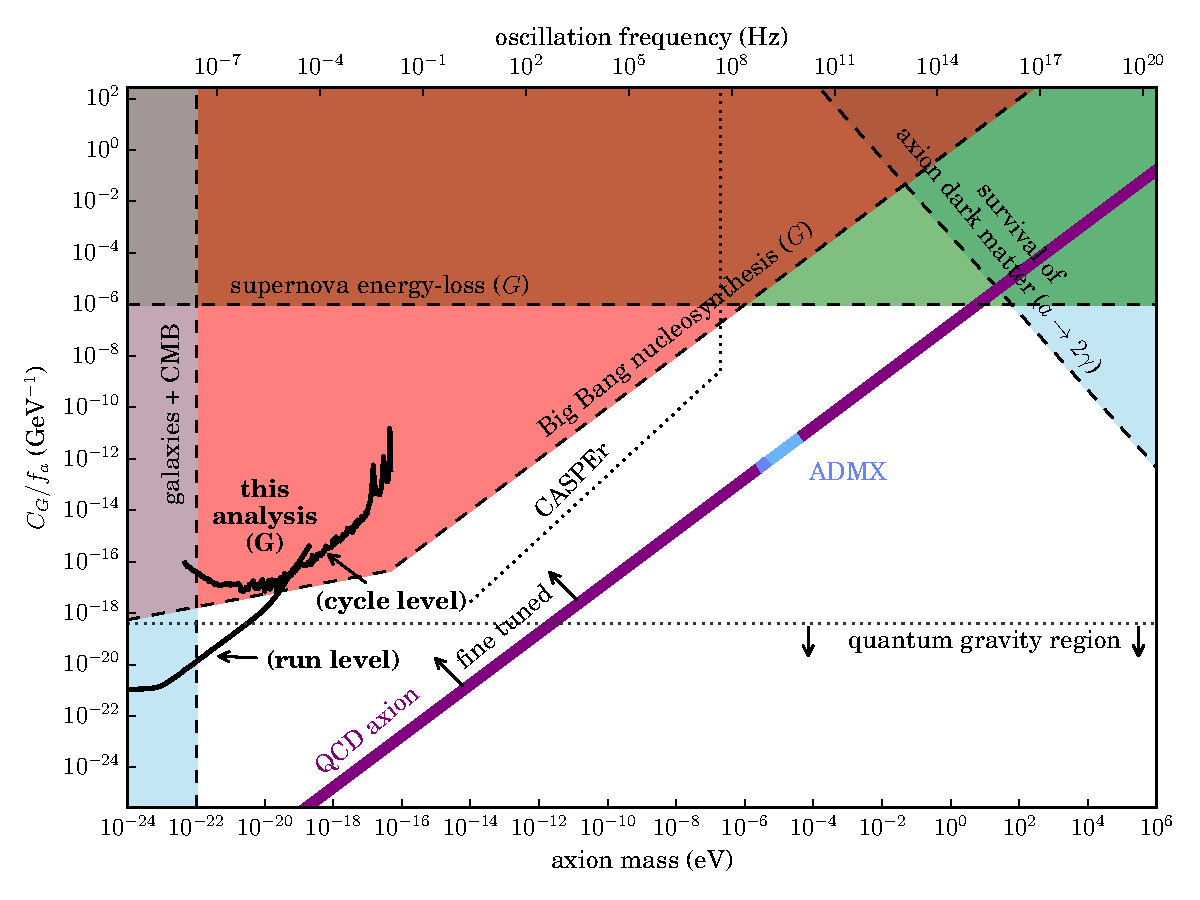
\includegraphics[width=\columnwidth]{gfx/axions/axion_limits_only_G}
  \caption{Our exclusion limits in the axion landscape. \note{MR: The limits plotted on this figure are slightly outdated. The cycle level includes only a subset of data. I think we should include a plot with limits on the nEDM oscillation itself (nEDM in 1e-26 ecm vs frequency). This is potentially of interest to a wider community. Also need to carefully decide which other limits to include on the plot.}}
  \end{center}
\end{figure}

An upper limit on the mass of axions, which saturate the observed cold DM content and form an oscillating classical field, is set by the requirement that there are a large number of axions within the reduced de Broglie volume (i.e., $n_a \left( \lambda_{\textrm{dB}}/2\pi \right)^3 \gg 1$):~$m_a \lesssim 0.1$ eV.
Sufficiently low-mass and feebly-interacting axions can survive to the present day.
For the QCD axion, this requires $m_a \lesssim 24$ eV in order for the $a \to 2 \gamma$ decay channel to be sufficiently suppressed, while for more generic ALPs, the restriction is generally less severe, meaning that the upper mass bound $m_a \lesssim 0.1$ eV is readily satisfied (see, e.g., \cite{Fields2015ALP_decay}).
For $m_a \gtrsim 0.1$ eV, axions may contribute to hot DM (see, e.g., \cite{Archidiacono2013_hot_axion_DM}).

The simplest lower limit on the mass of axions, which saturate the observed cold DM content, comes from the requirement that their de Broglie wavelength not exceed the DM halo size of the smallest dwarf galaxies ($R \sim 1$ kpc):~$m_a \gtrsim 10^{-22}$ eV.
Ultra-low-mass axion DM only behaves like perfect cold DM on length scales larger than the axion de Broglie wavelength.
On shorter length scales, their gravitational collapse is prevented by the gradient energy in the axion field \cite{Khlopov1985}.
This characteristic feature of ultra-low-mass axion DM has non-trivial consequences for cosmology.
In particular, if axions saturate the observed DM content, then existing CMB measurements require $m_a \gtrsim 10^{-24}$ eV \cite{Marsh2015A}, while consistency with observed structure formation requires $m_a \gtrsim 10^{-22}$ eV \cite{Marsh2015B,Schive2015}.

Due to its effects on structure formation, ultra-low-mass axion DM in the mass range $10^{-24}~\textrm{eV} \lesssim m_a  \lesssim 10^{-20}$ eV has been proposed to resolve several long-standing ``small-scale crises'' of the cold DM model \cite{Hu2000,Marsh2014,Paredes2015}.
In the future, cosmological observations may be able to distinguish ultra-low-mass axion DM with masses $m_a \lesssim 10^{-18}~\textrm{eV}$ from standard cold DM \cite{Marsh2015C}. Gravitational wave astronomy \cite{LIGO2016} has the potential to discover signals due to black hole superradiance caused by axions in the mass range $10^{-18}~\textrm{eV} \lesssim m_a  \lesssim 10^{-12}$ eV \cite{Marsh2015Review,Arvanitaki2010}.

The most stringent astrophysical limits on the axion-gluon coupling for the axion masses of interest in the present work come from Big Bang nucleosynthesis (BBN).
At second order, the axion-gluon coupling in Eq.~(\ref{Axion_couplings}) increases the neutron-proton mass difference via the effective operator $\mathcal{L}_{\textrm{eff}} = (f_\pi \bar{g}^{(0)}_{\pi N N} / 2) (m_d - m_u)/ (m_d + m_u) (C_G a / f_a)^2 \bar{N} \tau^3 N$:~$\delta Q_{np} \approx 0.37~\textrm{MeV}~\left(C_G a / f_a \right)^2$ \cite{Ubaldi2010,Blum2014}, altering the primordial abundances of light elements produced during BBN.
Comparison of measurements and SM calculations of the primordial $^4$He abundance gives the following rough constraints \cite{Blum2014}:
\begin{eqnarray}
\label{aGG_BBN_limits}
\frac{m_a^{1/4} f_a}{ C_G} \gtrsim 10^{10}~\textrm{GeV}^{5/4}, ~ \textrm{$m_a \ll 10^{-16}$ eV },\\
\frac{m_a f_a}{ C_G} \gtrsim 10^{-9}~\textrm{GeV}^2, ~ \textrm{$m_a \gg 10^{-16}$ eV },
\end{eqnarray}
assuming that axions saturate the present-day DM content.
The axion-gluon coupling also induces the following effective operator via the process shown in Fig.~1a:~$\mathcal{L}_{\textrm{eff}} = (-i g^d_N / 2) a \bar{N} \sigma_{\mu \nu} \gamma_5 N F^{\mu \nu}$, with $g^d_n \approx (2.4 \times 10^{-16} C_G / f_a) ~ e \cdot \textrm{cm} = (3.7 \times 10^{-3} C_G / f_a) ~\textrm{GeV}^{-1}$ and $g^d_n \simeq - g^d_p$.
Applying supernova energy-loss bound arguments to this effective operator for the process $N + \gamma \to N + a$ give the following rough constraint \cite{Graham2013}:
\begin{equation}
\label{aGG_SN_limits}
\frac{f_a}{C_G} \gtrsim 10^6 ~\textrm{GeV}, ~ \textrm{$m_a \lesssim 3 \times 10^{7}$ eV} \, ,
\end{equation}
which is significantly weaker than the above BBN constraints for the mass range of interest in the present work.


The most stringent astrophysical limits on the axion-nucleon couplings come from supernova energy-loss bound arguments applied to the bremsstrahlung channel $N + N \to N + N + a$, which give the rough constraint (see \cite{Raffelt2008LNP} and the references therein):
\begin{equation}
\label{aNN_SN_limits}
\frac{f_a}{C_N} \gtrsim 10^9 ~\textrm{GeV}, ~\textrm{$m_a \lesssim 3\times 10^{7}$ eV} \, .
\end{equation}
The most stringent laboratory limits on the axion-neutron coupling come from a K$/^{3}$He co-magnetometry search for new spin-dependent forces mediated by virtual axion exchange \cite{Romalis2009_NF}:
\begin{equation}
\label{ann_lab_limits}
\frac{f_a}{C_n} > 1 \times 10^4 ~\textrm{GeV}, ~\textrm{$m_a \lesssim 10^{-7}$ eV} \, ,
\end{equation}
while the most stringent laboratory limits on the axion-proton coupling come from a H$_{2}$ spectroscopy search for analogous new spin-dependent forces \cite{Romalis2009_NF,Ramsey1979}:
\begin{equation}
\label{app_lab_limits}
\frac{f_a}{C_p} > 60 ~\textrm{GeV}, ~\textrm{$m_a \lesssim 10^{5}$ eV}  \, .
\end{equation}


The most stringent astrophysical limits on the axion-electron coupling come white dwarf cooling arguments applied to the bremsstrahlung channel $e^{-} + (Z,A) \to e^{-} + (Z,A) + a$, which give the rough constraint (see \cite{Raffelt2008LNP} and the references therein):
\begin{equation}
\label{aee_WD_limits}
\frac{f_a}{C_e} \gtrsim 10^{10} ~\textrm{GeV}, ~\textrm{$m_a \lesssim 10^3$ eV} \, .
\end{equation}
The most stringent laboratory limits on the axion-electron coupling come from a rotating torsion pendulum search for new spin-dependent forces mediated by virtual axion exchange \cite{Adelberger2013}:
\begin{equation}
\label{aee_lab_limits}
\frac{f_a}{C_e} > 3 \times 10^4 ~\textrm{GeV}, ~\textrm{$m_a \lesssim 10^{-7}$ eV} \, .
\end{equation}


%%%%%%%%%%%
\textbf{Appendix B:~Model for Ultra-low-mass Axions with $C_G\sim 1$.} ---
Here we sketch a model, for which $C_G\sim 1$, but which also satisfies $m_af_a\ll C_G\Lambda_{\mathrm{QCD}}^2$. Ref.~\cite{Blum2014} showed that such a model could not be achieved via the mass mixing of two axions coupled to the QCD sector, with an additional UV mass source.
Our model, on the other hand, has a single axion with two non-perturbative sources of mass. Consider the following Lagrangian (note that we supress the index summation here):
\begin{equation}
\label{Hidden-QCD_L}
\mathcal{L}\supset \frac{C_G}{f_a}\frac{g}{32 \pi^2}a G\tilde{G}+\frac{C_X}{f_a}\frac{g_X}{32 \pi^2}a X\tilde{X} \, ,
\end{equation}
where $X$ is the gauge field strength of some confining, non-Abelian, CP-violating hidden sector.
The gauge coupling is $g_X$, and the hidden-sector quarks that are charged in $X$ give rise to a $C_X$-anomaly under the Peccei-Quinn symmetry.

The first term in Eq.~(\ref{Hidden-QCD_L}) gives rise to the usual axion potential due to QCD instantons.
Since QCD is CP-conserving in the absence of instantons, this potential is minimised at $a=0$ \cite{Vafa1984}.
The potential due to instantons in $X$, however, will be minimised at some other value, in general causing CP violation.
Consider the following axion potential at low energies when the QCD sector and the hidden sector are both in the confining phase:
\begin{align}
V(a) &= \Lambda_{\mathrm{QCD}}^4 \left[1- \cos \left(\frac{C_G a}{f_a}\right) \right] \notag \\
&+ \Lambda_{\mathrm{X}}^4 \left[1- \cos \left(\frac{C_X a}{f_a} + \delta \right)\right] \, ,
\end{align}
where $\Lambda_{\mathrm{QCD}} \approx 250$ MeV is the QCD scale and $\Lambda_X$ is the strong coupling scale of the hidden sector.
If the hidden sector strongly violates the CP symmetry, then one can have $\delta=\pi$, %{\color{red} what is the case for SU(2)?}
in which case the axion mass around the $a=0$ vacuum is given by:
\begin{equation}
m_a^2 = m_{\mathrm{QCD}}^2 (1-r^4) \, .
\end{equation}
where $m_{\mathrm{QCD}} = C_G\Lambda_{\mathrm{QCD}}^2/f_a$ and $r=(\Lambda_X C_X^{1/2})/(\Lambda_{\mathrm{QCD}}C_G^{1/2})$.
With sufficient fine-tuning of the ratio $r$, it is possible to construct a model with an ultra-low-mass axion, which produces a significantly larger oscillating neutron EDM and significantly larger oscillating atomic EDMs (generated via hadronic mechanisms), compared with the QCD axion.
If $r^4<1$ and $\delta=\pi$, the minimum of the potential exactly conserves the CP symmetry, leading to EDMs that oscillate about zero at a low frequency.
If $r^4>1$, and/or if $0<\delta<\pi$, the potential violates the CP symmetry, and an EDM oscillates about a non-zero value.

The fine-tuning in this model is related to the fine-tuning that defines the strong CP problem, i.e., a cancellation between CP-violating effects in different non-Abelian sectors.
This model is not intended to solve the strong CP problem, but to provide a setting in which the $\theta_{\textrm{QCD}}$ angle of QCD oscillates with a low frequency.
An observation of a low-frequency oscillating EDM of the neutron would present a fine-tuning problem for axion models.




\textbf{Appendix C:~Validation of analysis techniques and code} ---

The analysis of the ILL and PSI datasets was performed by two separate codes, with the ILL code written mostly by Nick in Python and the PSI code written mostly by Michał in Julia. None of the code used for calculations is shared between the programs or based on the code of the other program. However, both codes do implement the same analysis technique.

We want to ensure two things:
\begin{itemize}
\item {The codes are implementing the algorithms correctly}
\item {The algorithms are correct to give good results}
\end{itemize}

To accomplish the first objective we analyse the same datasets using both the ILL and PSI codes. To accomplish the second we compare some of the results of the simpler ILL analysis to analytical predictions where these exist.

\textbf{Appendix D:~How we determined how many Monte-Carlo samples were needed}

\section{Comparison of the two analyses}
\label{Sec:comparison}
The two analyses, long and short time--base, were developed as two separate codes. First by Nicholas Ayres, second by Michal Rawlik. However, the mathematical foundation of both is the same and it is, therefore, expected that the two implementations, given the same input, should give the same results.

Nine fake time series (\emph{datasets}) have been generated. For each dataset a set of frequencies to analyse has been agreed on. The long time--base analysis has been modifed to fit a constant offset in the LSSA fits. For each dataset we compare the \emph{detection} analysis and determination of the exclusion region in the signal space. The comparison in the detection analysis is presented in Fig.\,\ref{fig:comparison_detection}, where we compare:
\begin{enumerate}
  \item The periodogram of the dataset --- here we observe an agreement on  the $10^{-6}$ level.
  \item The average periodogram for the null hypothesis --- here we observe a 40\% disagreement for the lowest tested frequency. For all other frequencies the agreement is better then 4\% and is clearly dominated by numerical noise (which can be decreased by using more Monte Carlo samples.)
  \item The 1-, 2-, 3-, 4- and 5-sigma false--alarm thresholds --- we observe the same situation as for the average periodogram for the null hypothesis.
\end{enumerate}
For the exclusion region determination we compare the p--value on the signal hypothesis exclusion on a space spanned by frequency and amplitude of the signal. The comparison is presented in Fig.\,\ref{fig:comparison_exclusion}. In most interesting region, the boundary between the black and white areas, we observe differences on the order of few per cent. Because the differences are not systematic, they are most likely caused by numeric noise.

\begin{figure*}[ptb]
  \centering 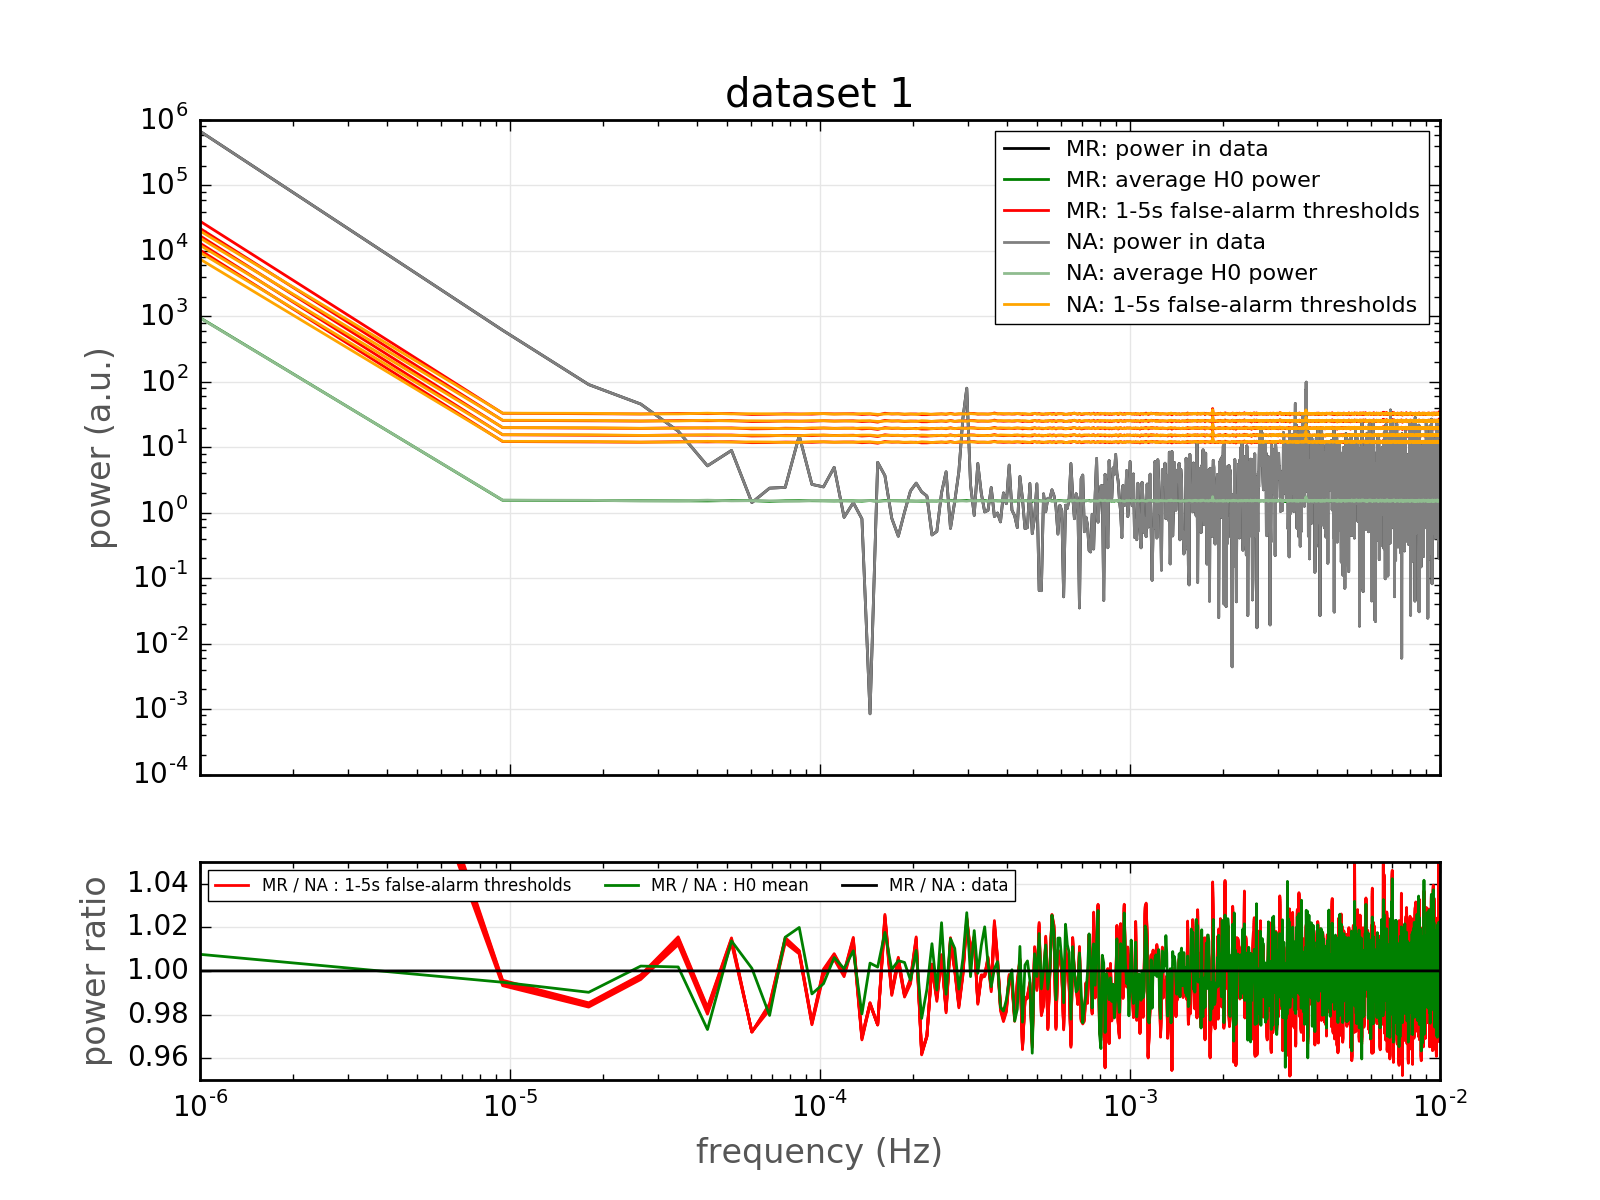
\includegraphics[width=0.32\linewidth]{gfx/axions/comparison/comparison_detection_dataset1.png}
  \centering 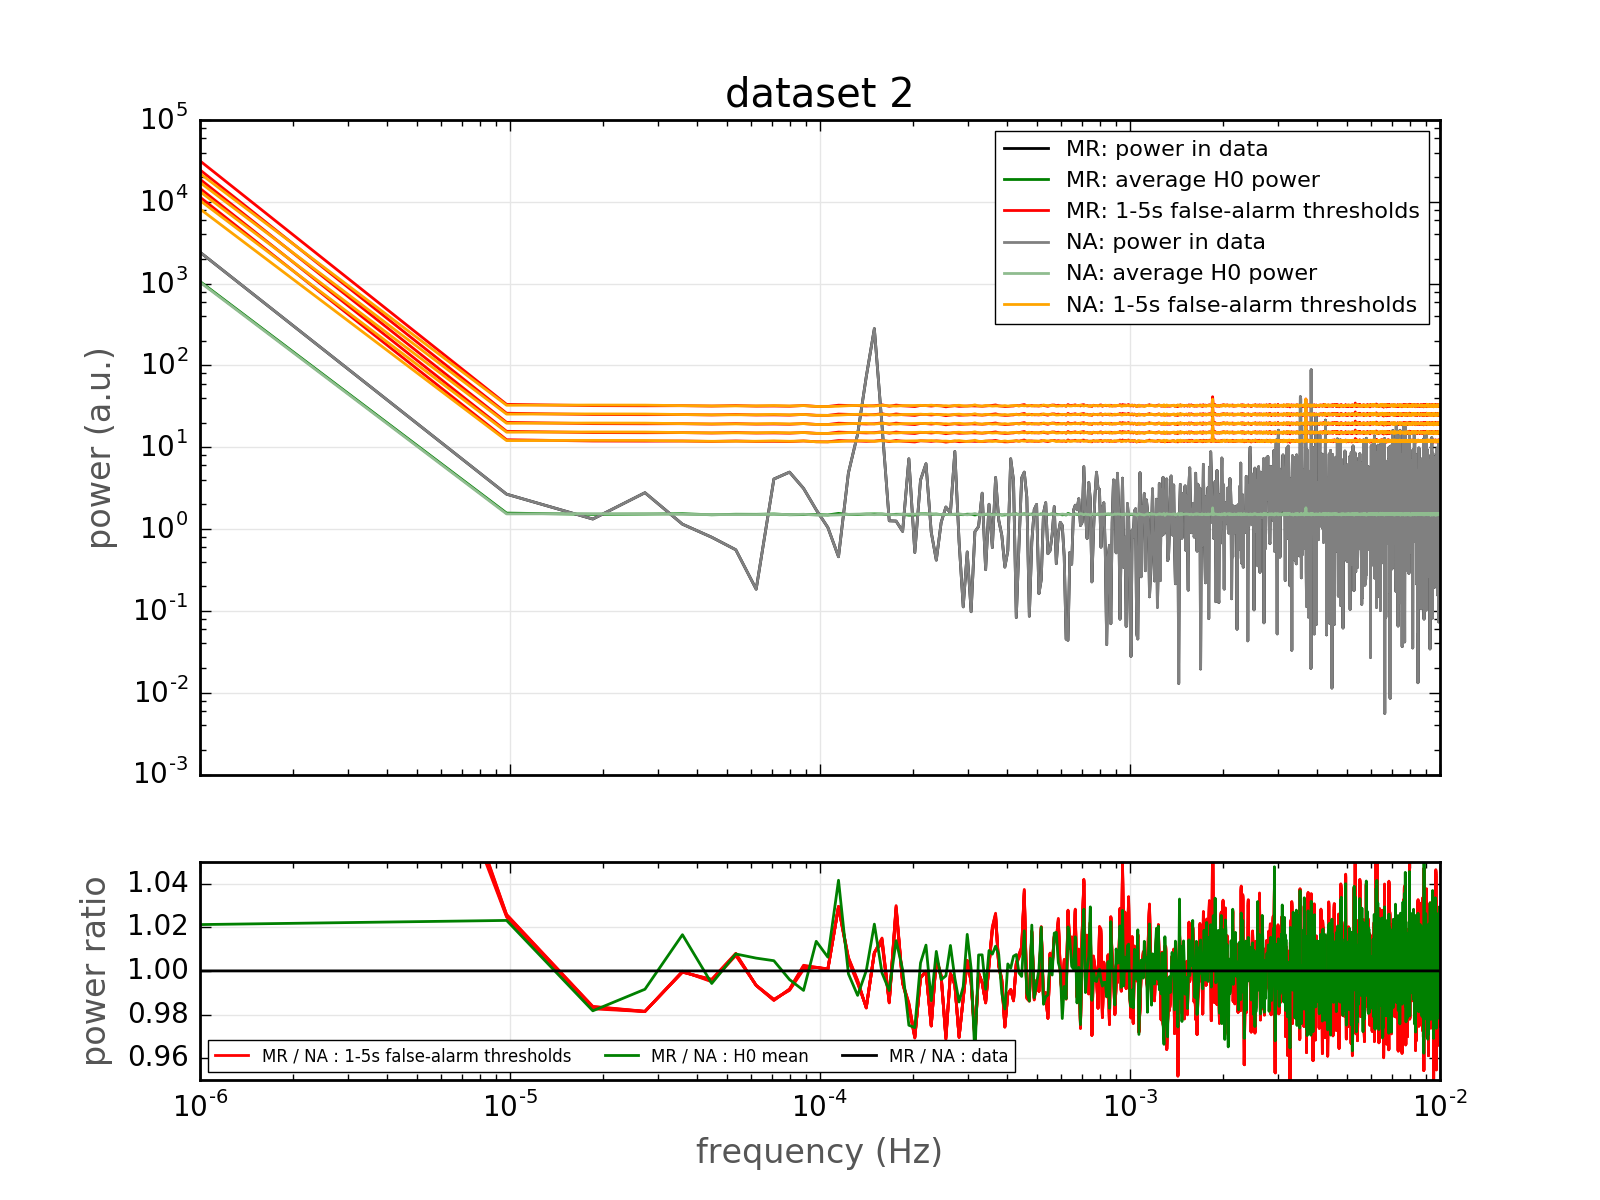
\includegraphics[width=0.32\linewidth]{gfx/axions/comparison/comparison_detection_dataset2.png}
  \centering 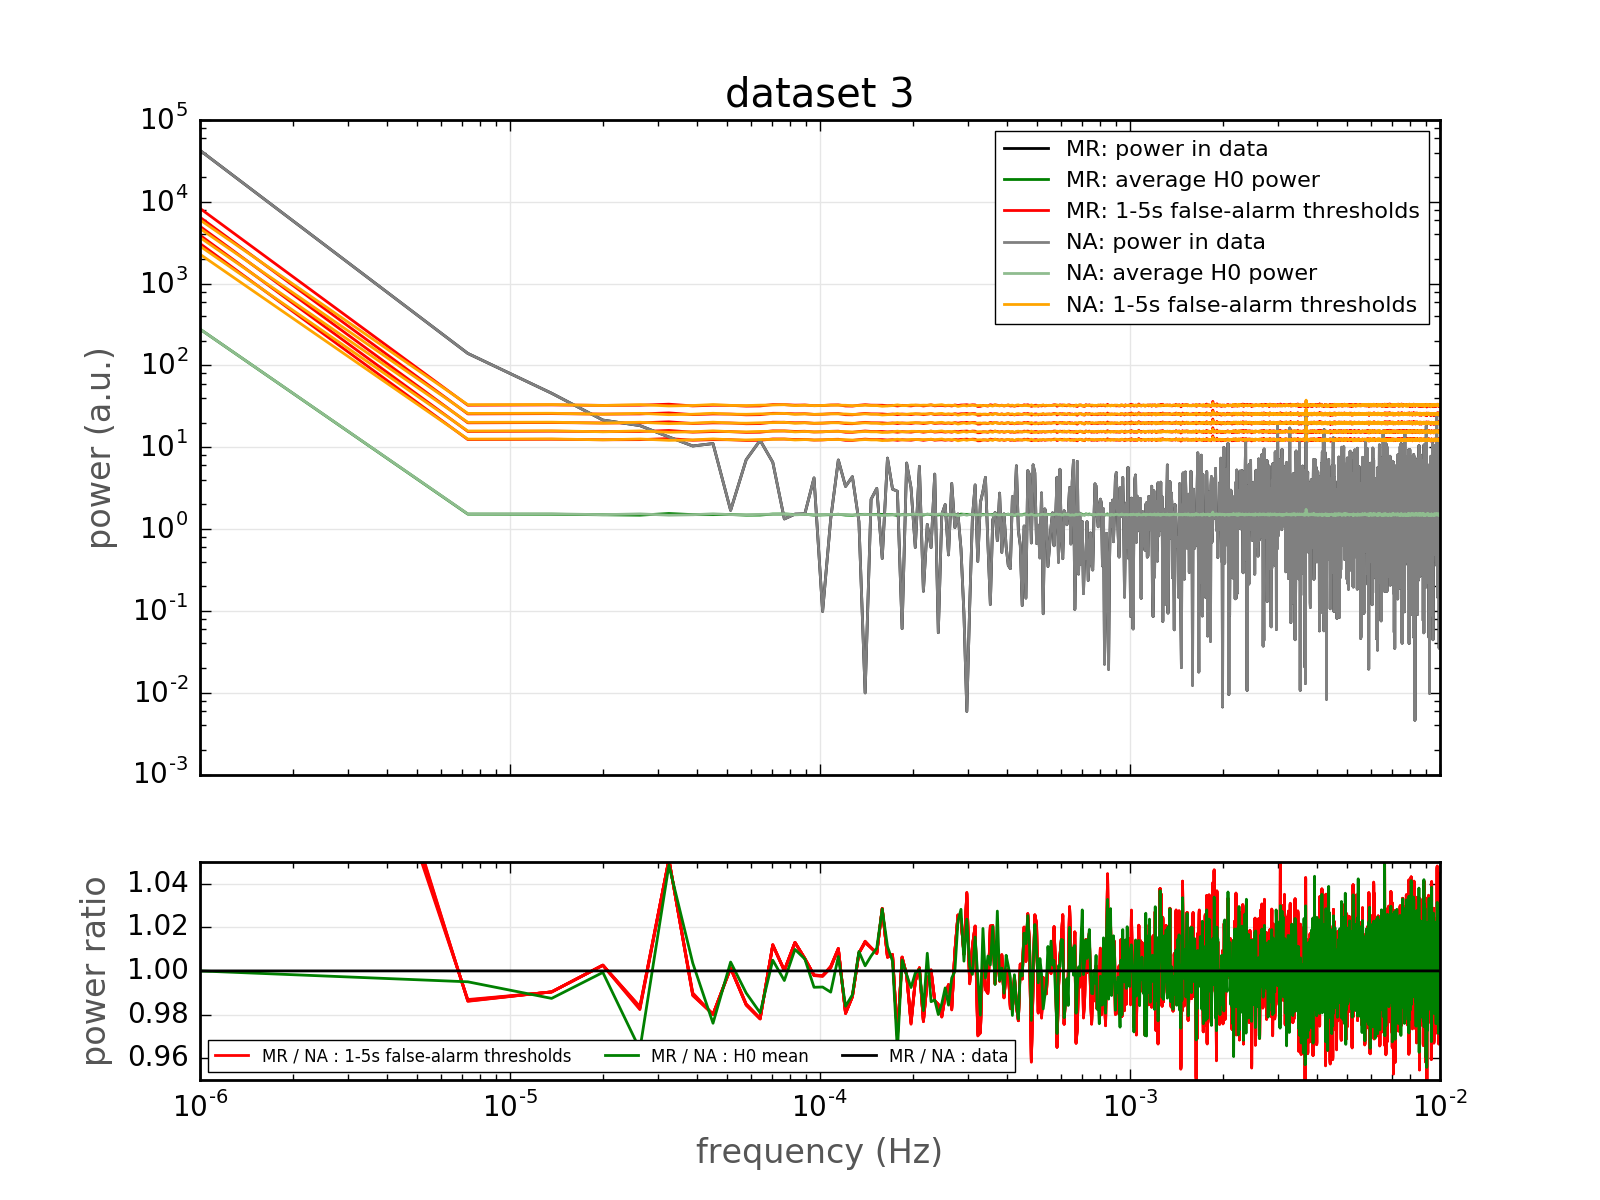
\includegraphics[width=0.32\linewidth]{gfx/axions/comparison/comparison_detection_dataset3.png}
  \centering 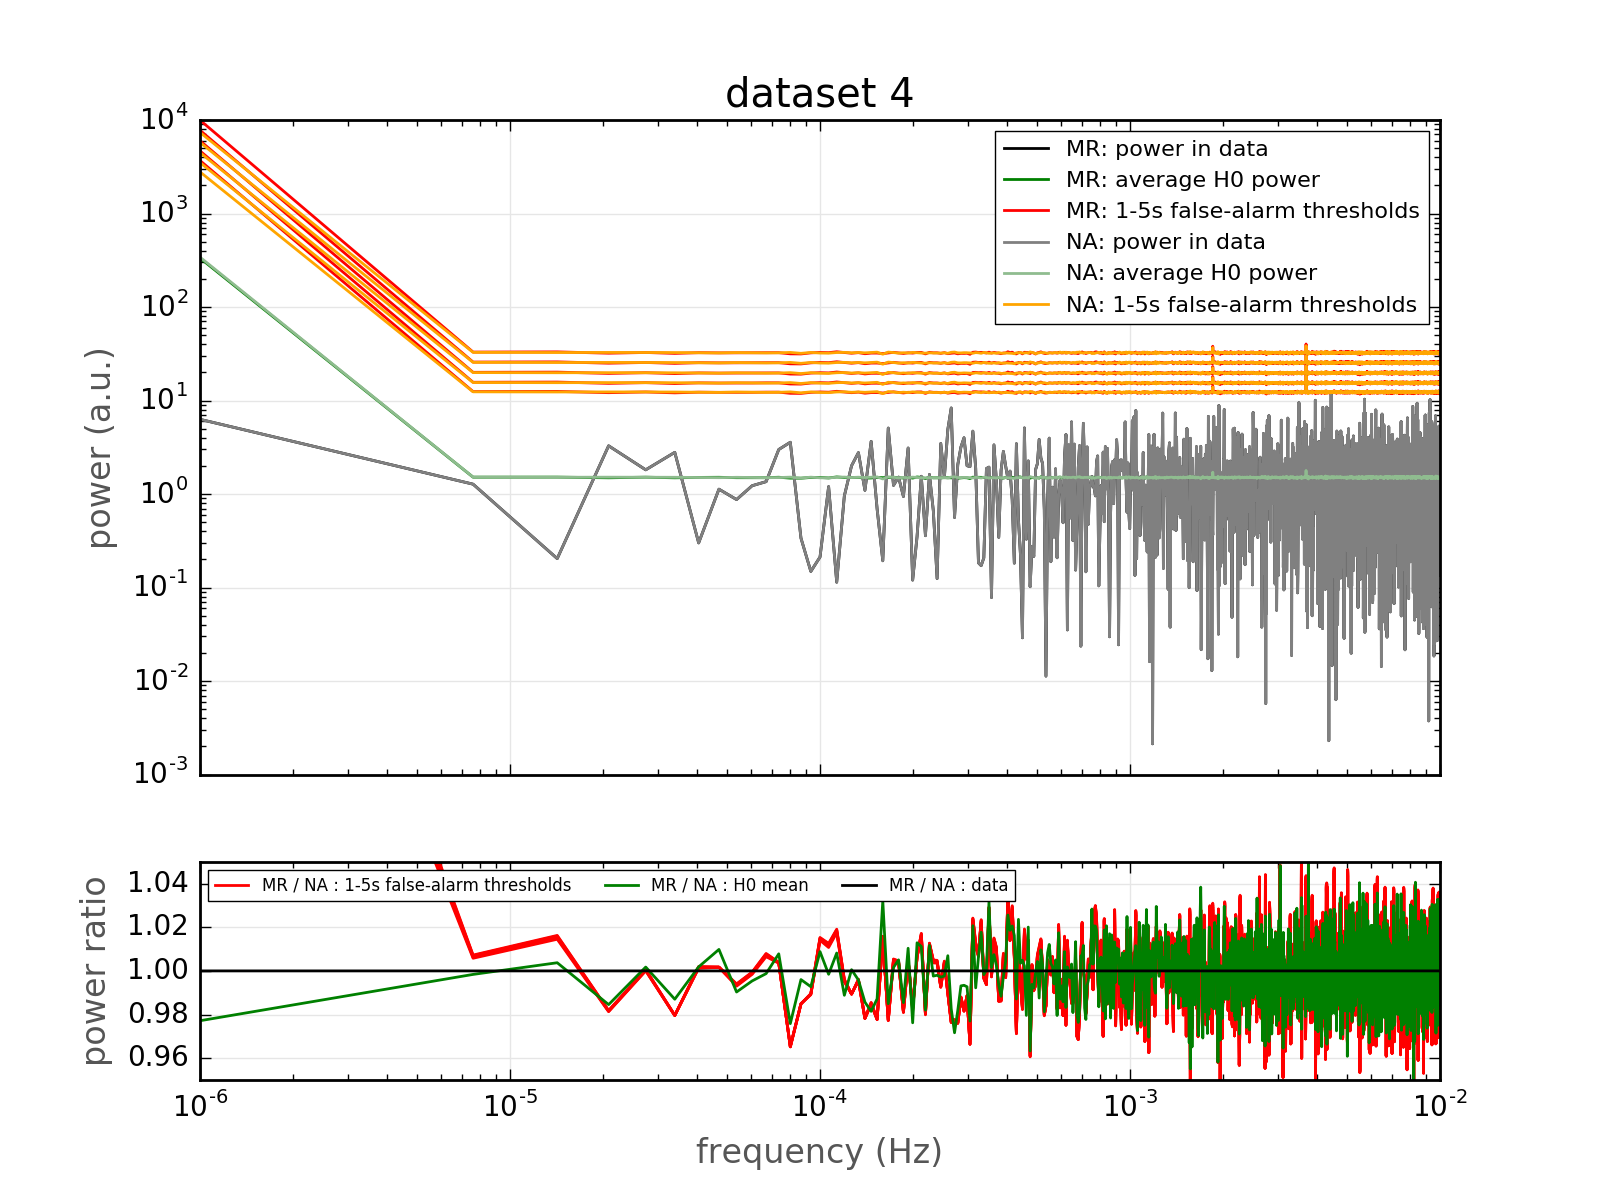
\includegraphics[width=0.32\linewidth]{gfx/axions/comparison/comparison_detection_dataset4.png}
  \centering 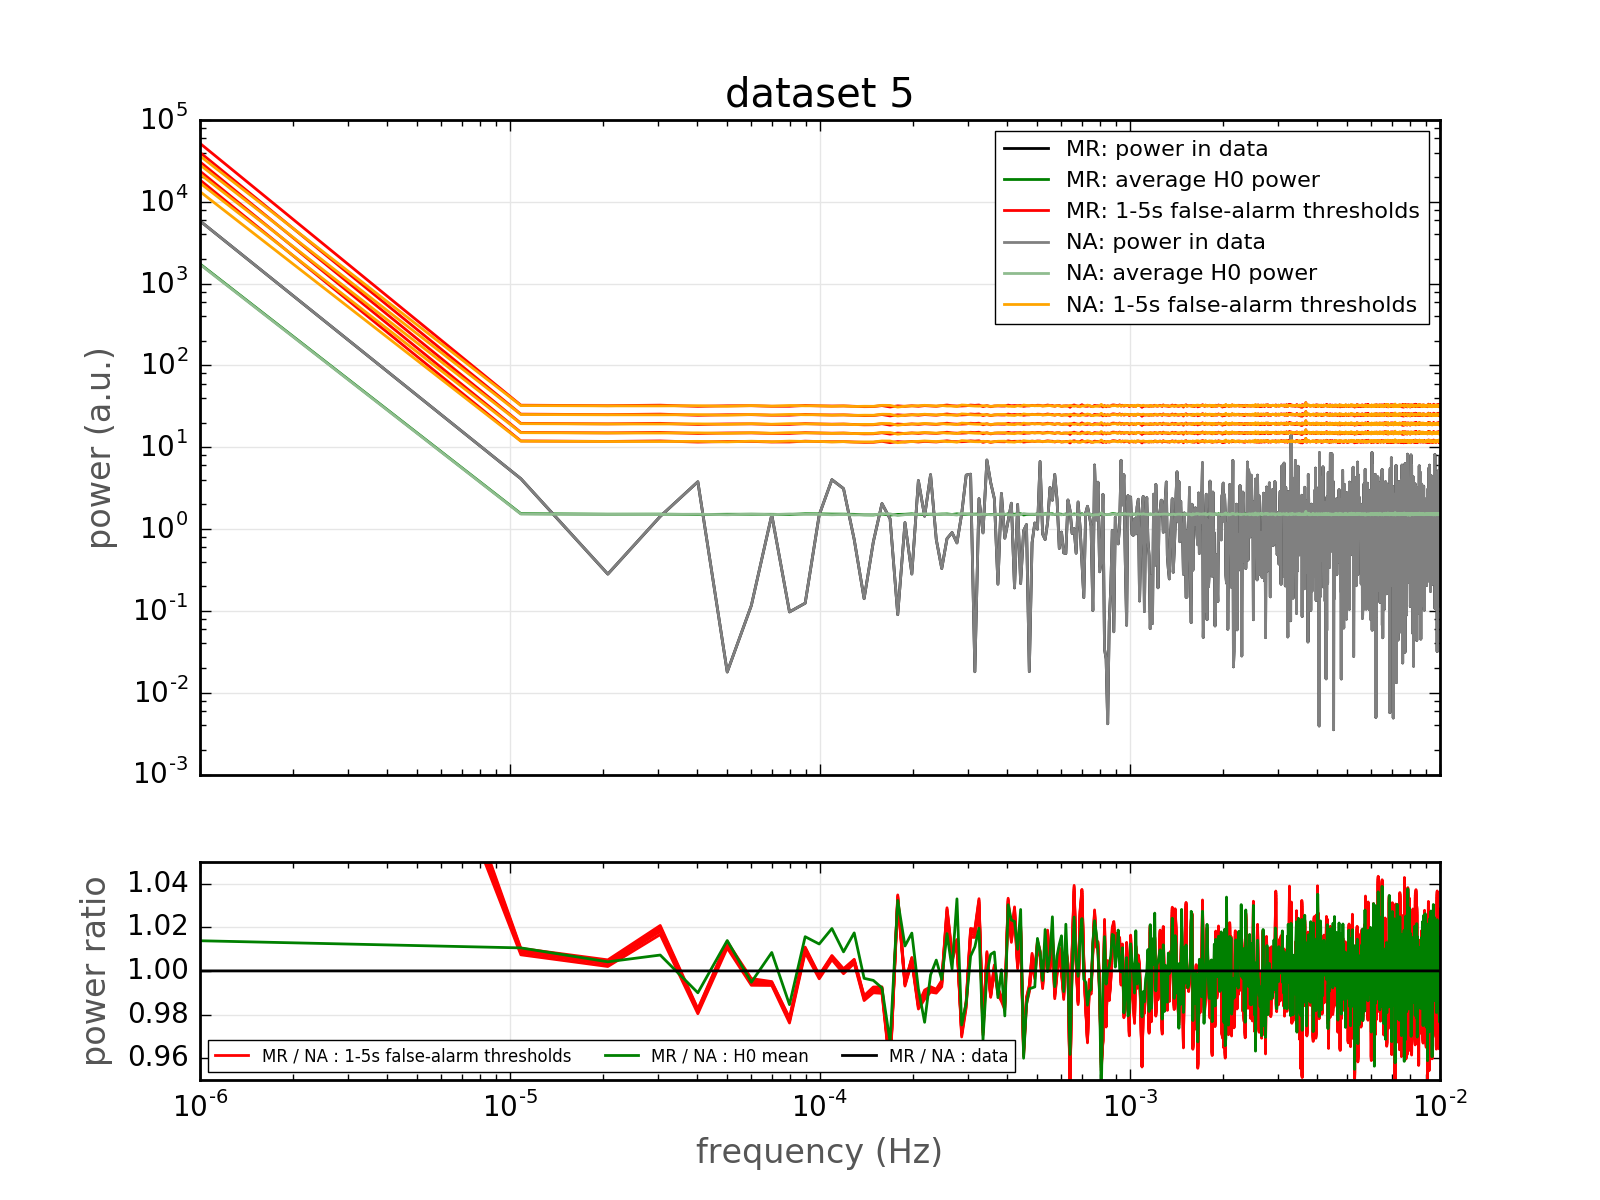
\includegraphics[width=0.32\linewidth]{gfx/axions/comparison/comparison_detection_dataset5.png}
  \centering 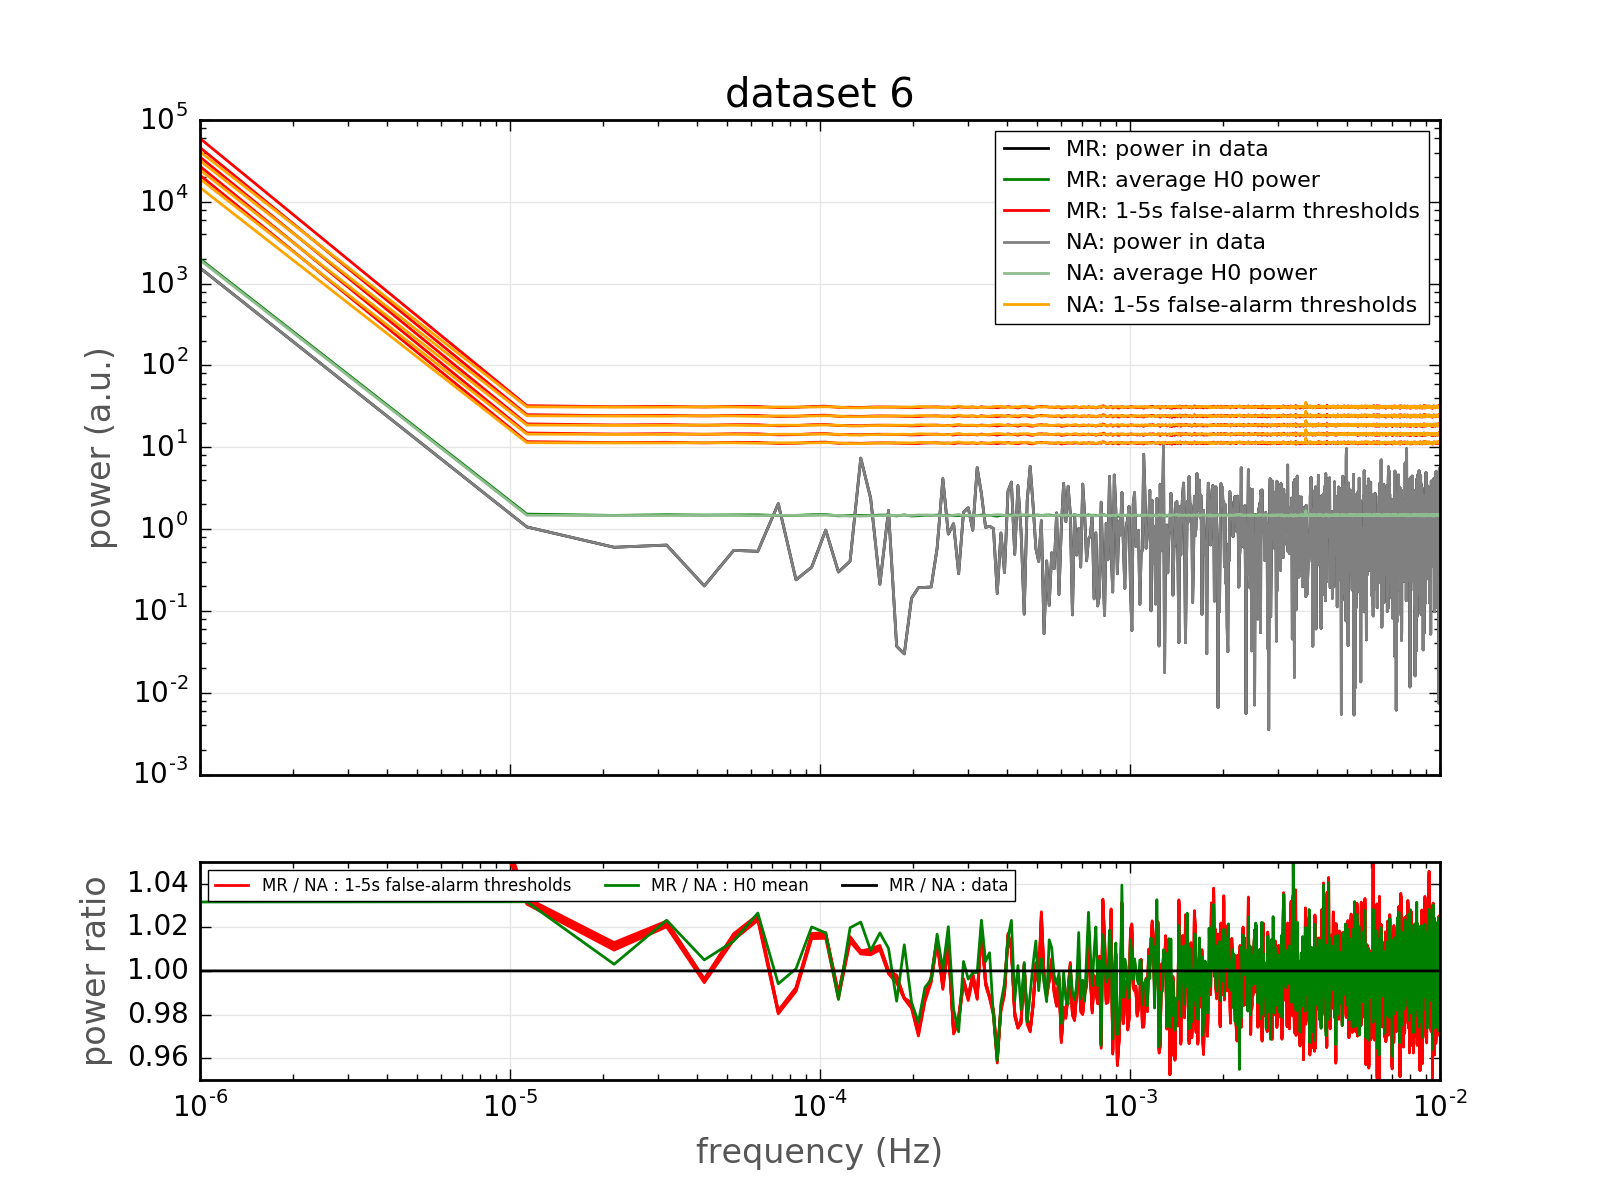
\includegraphics[width=0.32\linewidth]{gfx/axions/comparison/comparison_detection_dataset6.png}
  \centering 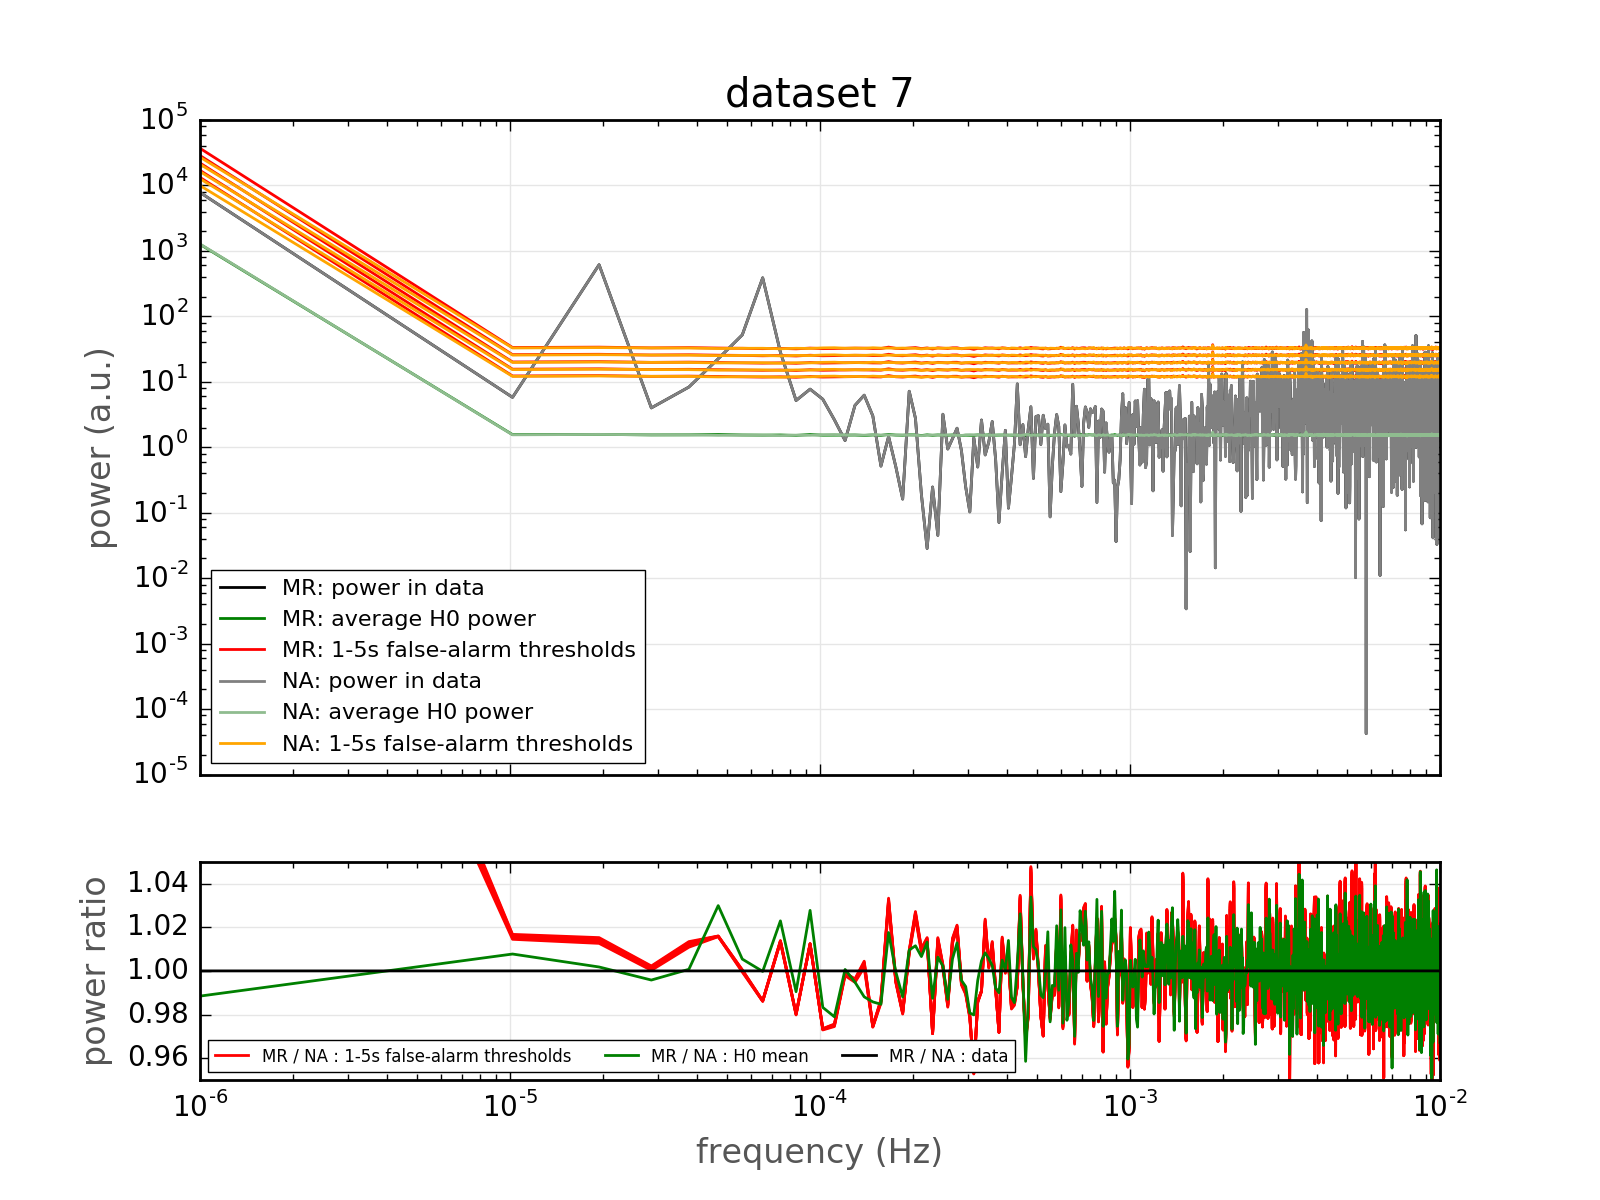
\includegraphics[width=0.32\linewidth]{gfx/axions/comparison/comparison_detection_dataset7.png}
  \centering 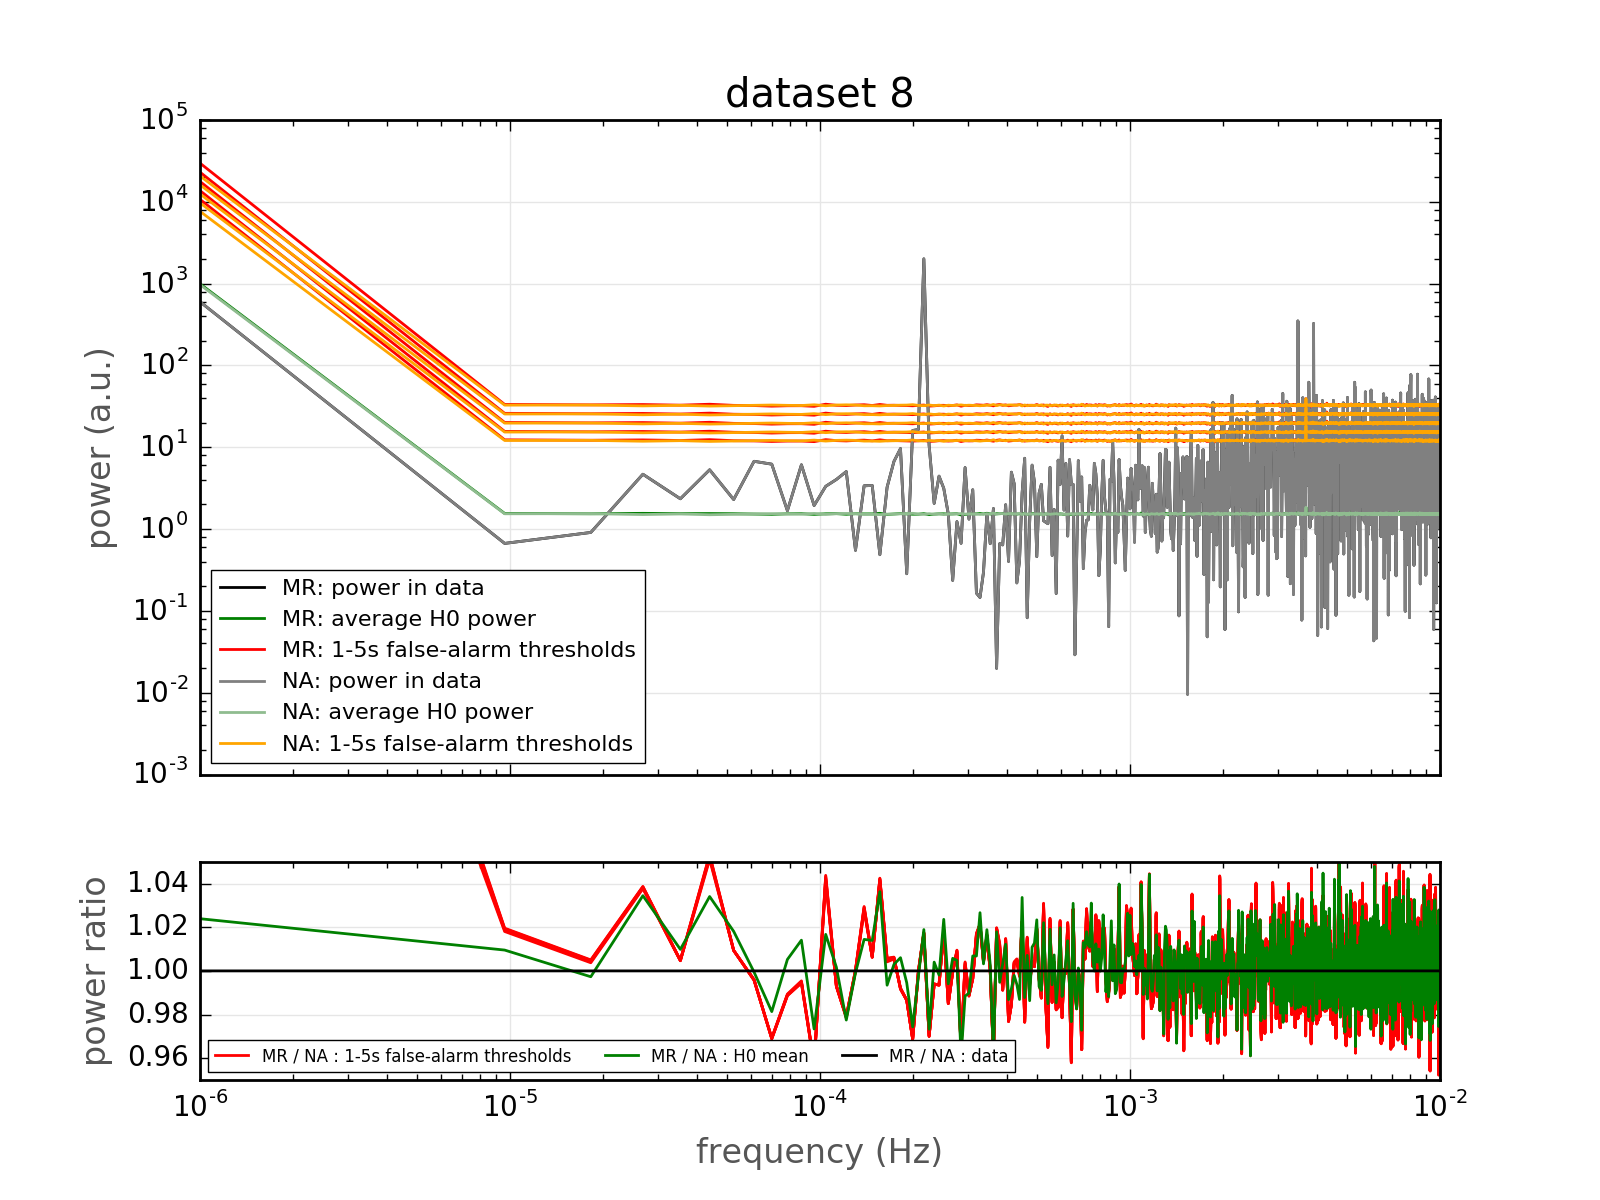
\includegraphics[width=0.32\linewidth]{gfx/axions/comparison/comparison_detection_dataset8.png}
  \centering 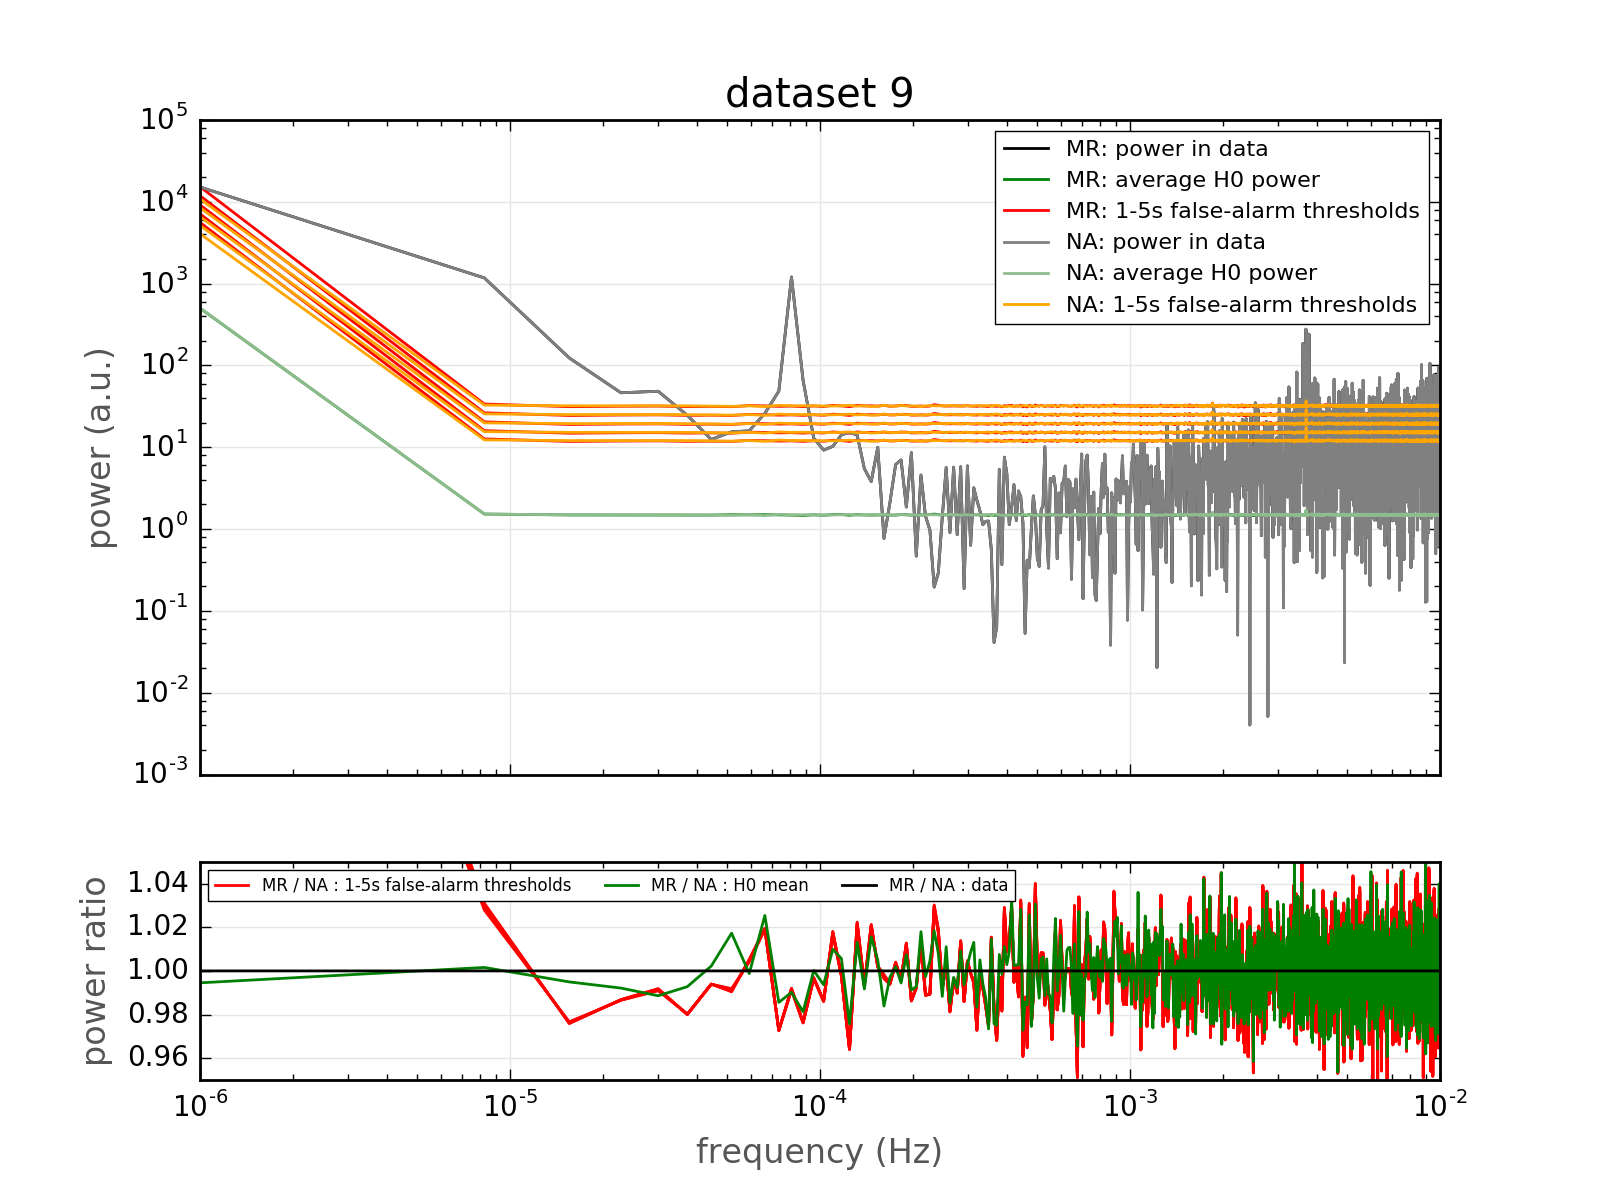
\includegraphics[width=0.32\linewidth]{gfx/axions/comparison/comparison_detection_dataset9.png}
  \caption{Comparison between the analysis implemented by Nicholas Ayres (NA) and Michal  Rawlik (MR). This figure presents the \emph{detection} part of the analysis. Each of the nine plots presents a direct comparison of one fake dataset. For both analyses the following is plotted: (a) the periodogram of the dataset, (b) the average periodogram for the null hypothesis, (c) the 1-,...,5-sigma false alarm thresholds. Below each plot the ratio of the corresponding curves for the two analyses is plotted. For the lowest tested frequency we observe a 40\% difference in the average power for the null hypothesis, as well as the false--alarm thresholds. This single point lies outside the plotted area. For all the other frequencies disagreement is dominated by numerical noise. The periodograms of the datasets agree on the $10^{-6}$ level.}
  \label{fig:comparison_detection}
\end{figure*}

\begin{figure*}[tb]
  \centering 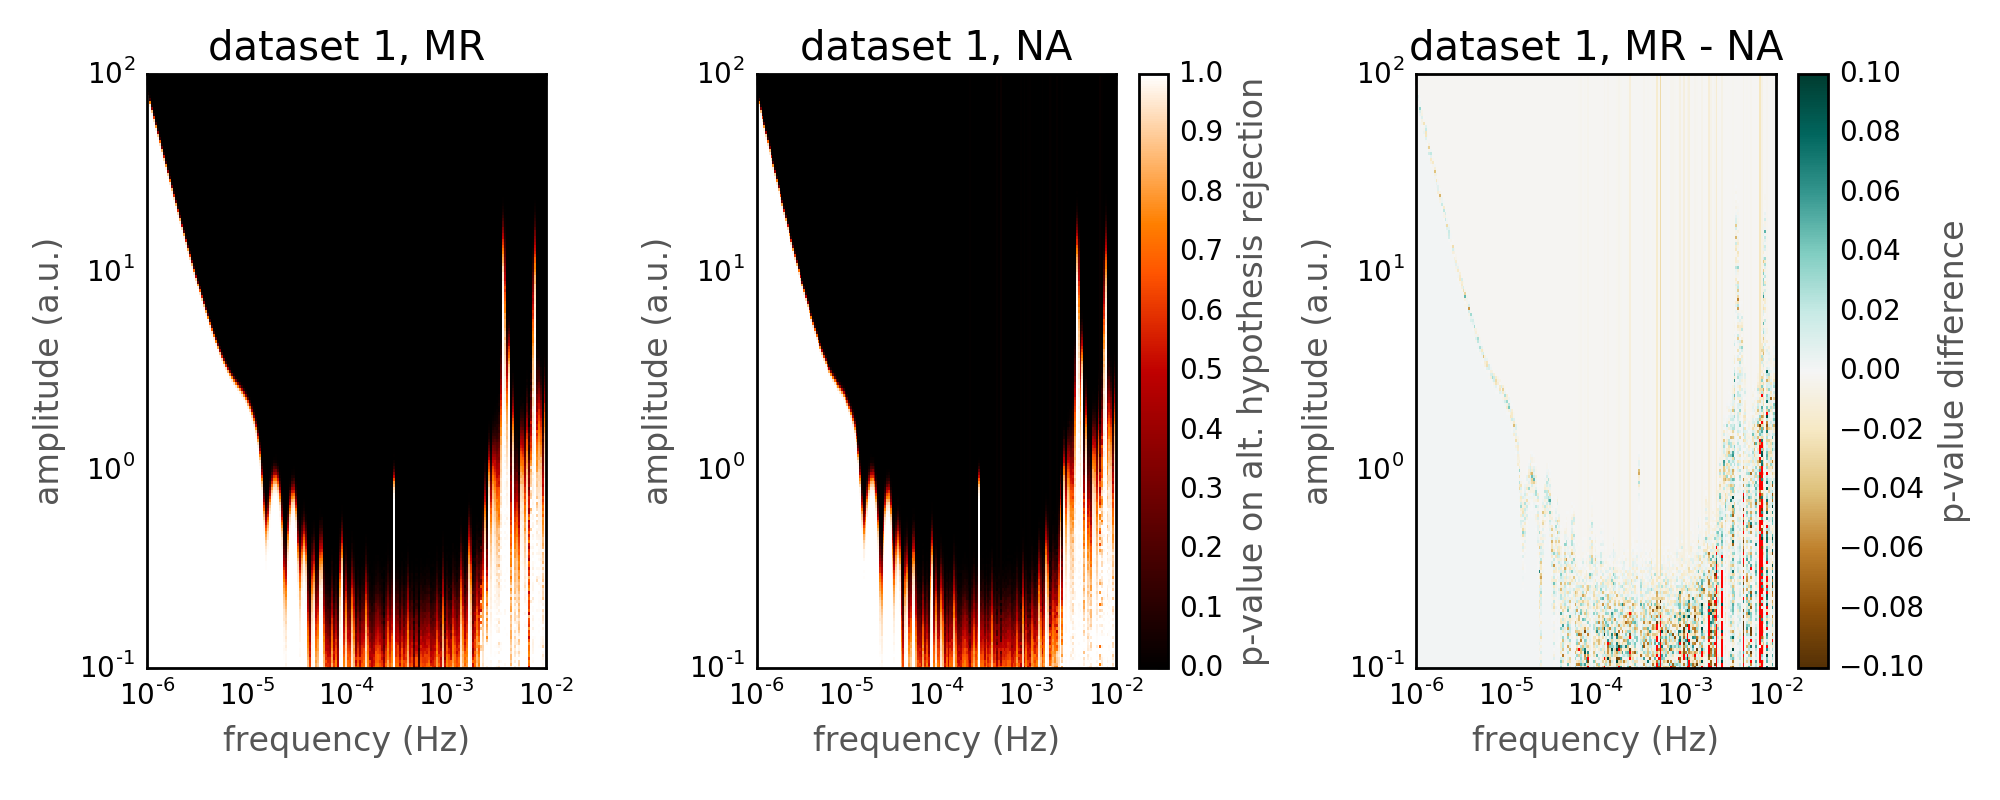
\includegraphics[width=0.45\linewidth]{gfx/axions/comparison/comparison_exclusion_dataset1.png}
  \centering 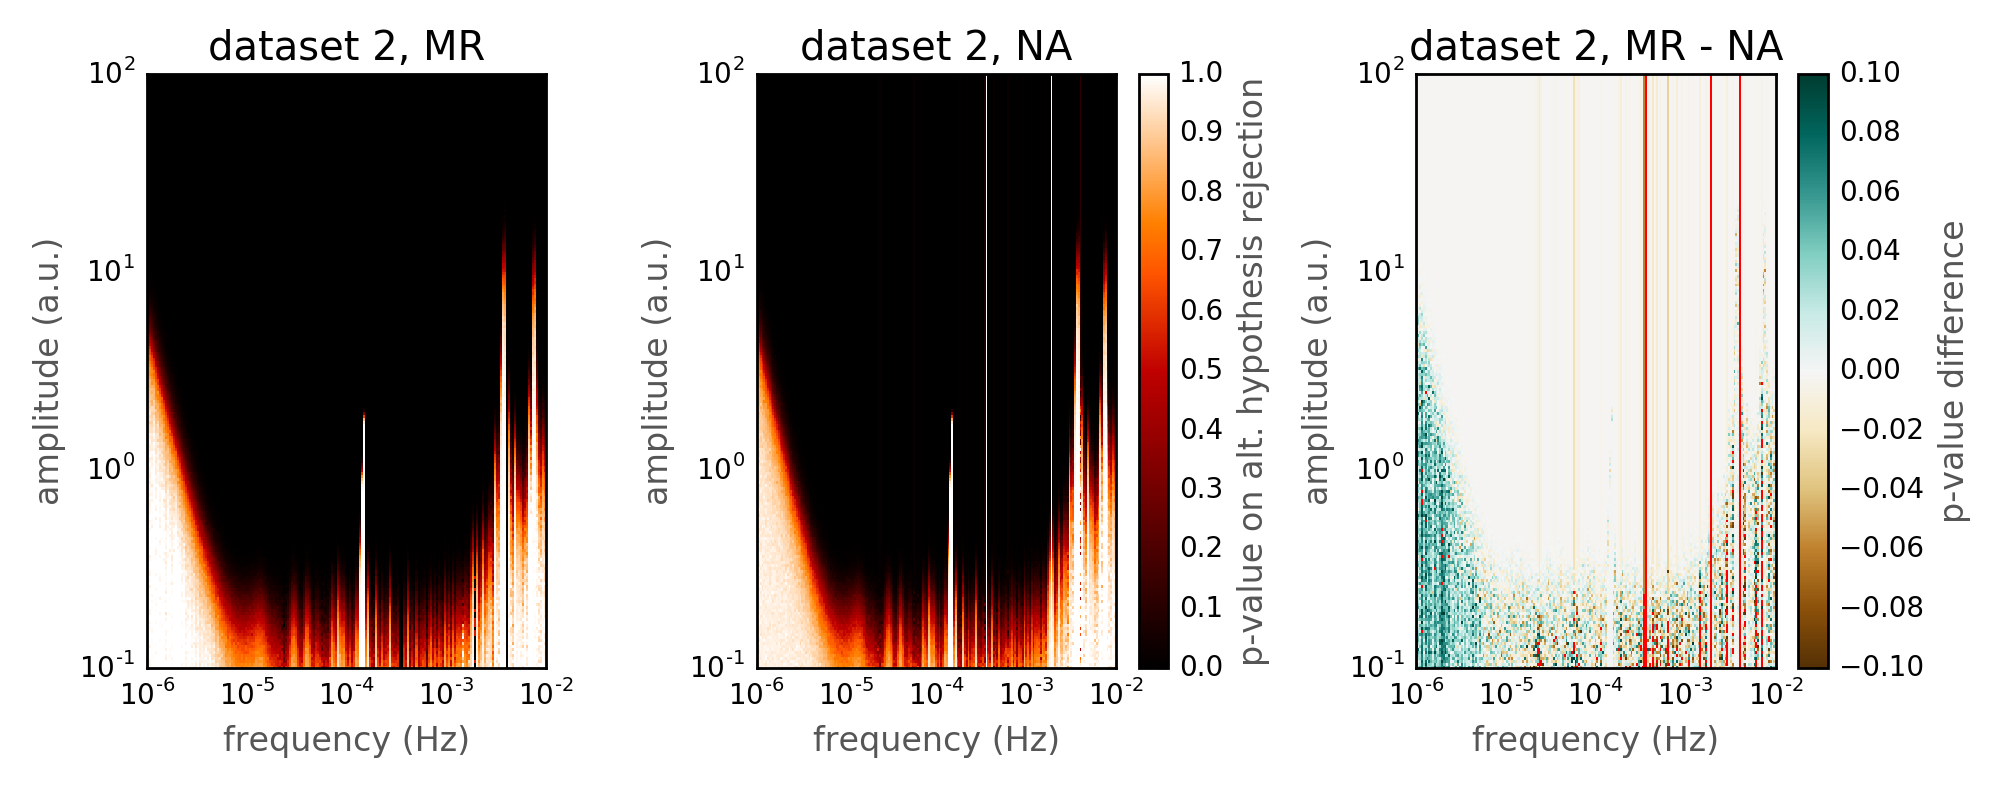
\includegraphics[width=0.45\linewidth]{gfx/axions/comparison/comparison_exclusion_dataset2.png}
  \centering 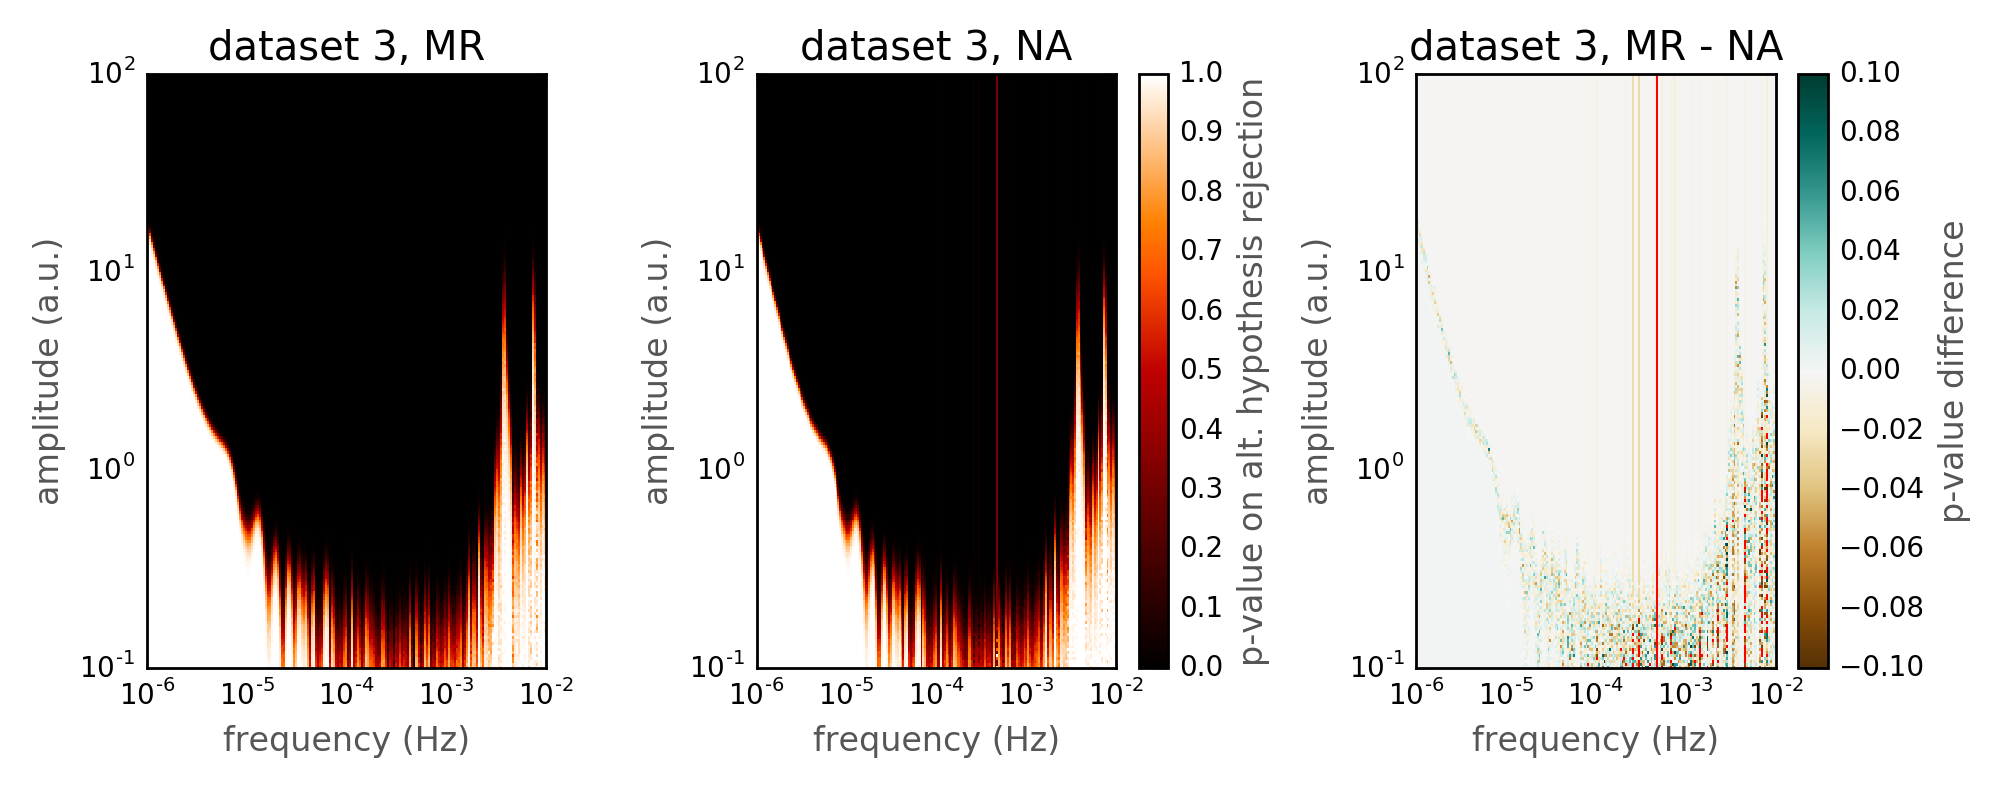
\includegraphics[width=0.45\linewidth]{gfx/axions/comparison/comparison_exclusion_dataset3.png}
  \centering 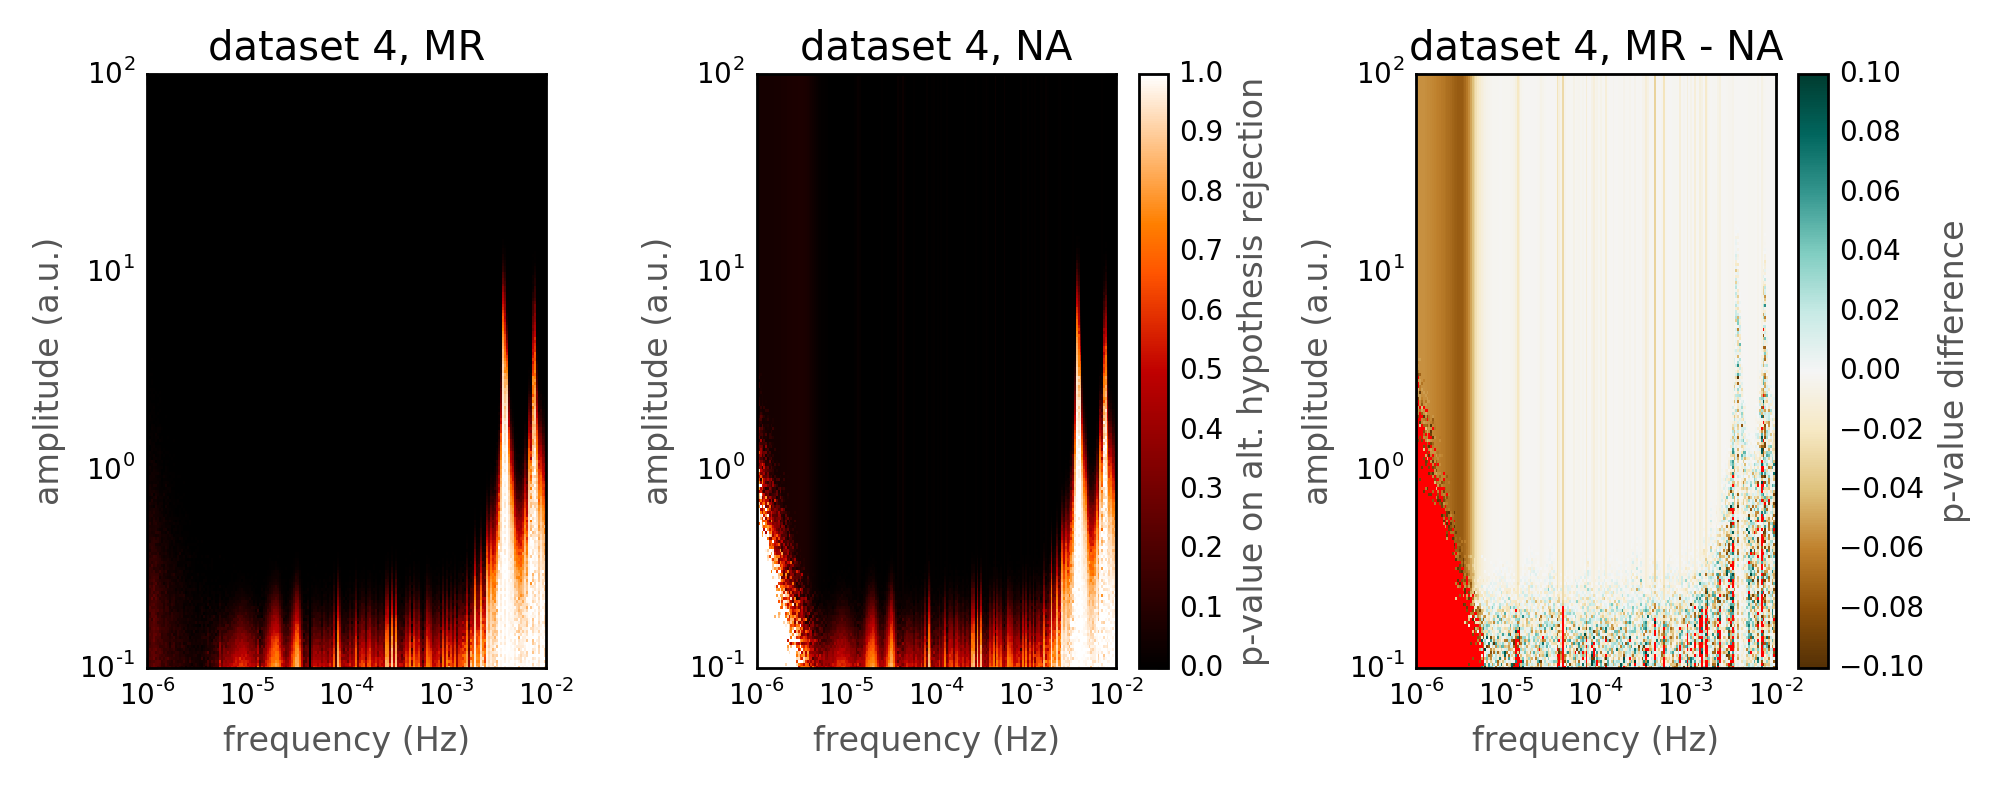
\includegraphics[width=0.45\linewidth]{gfx/axions/comparison/comparison_exclusion_dataset4.png}
  \centering 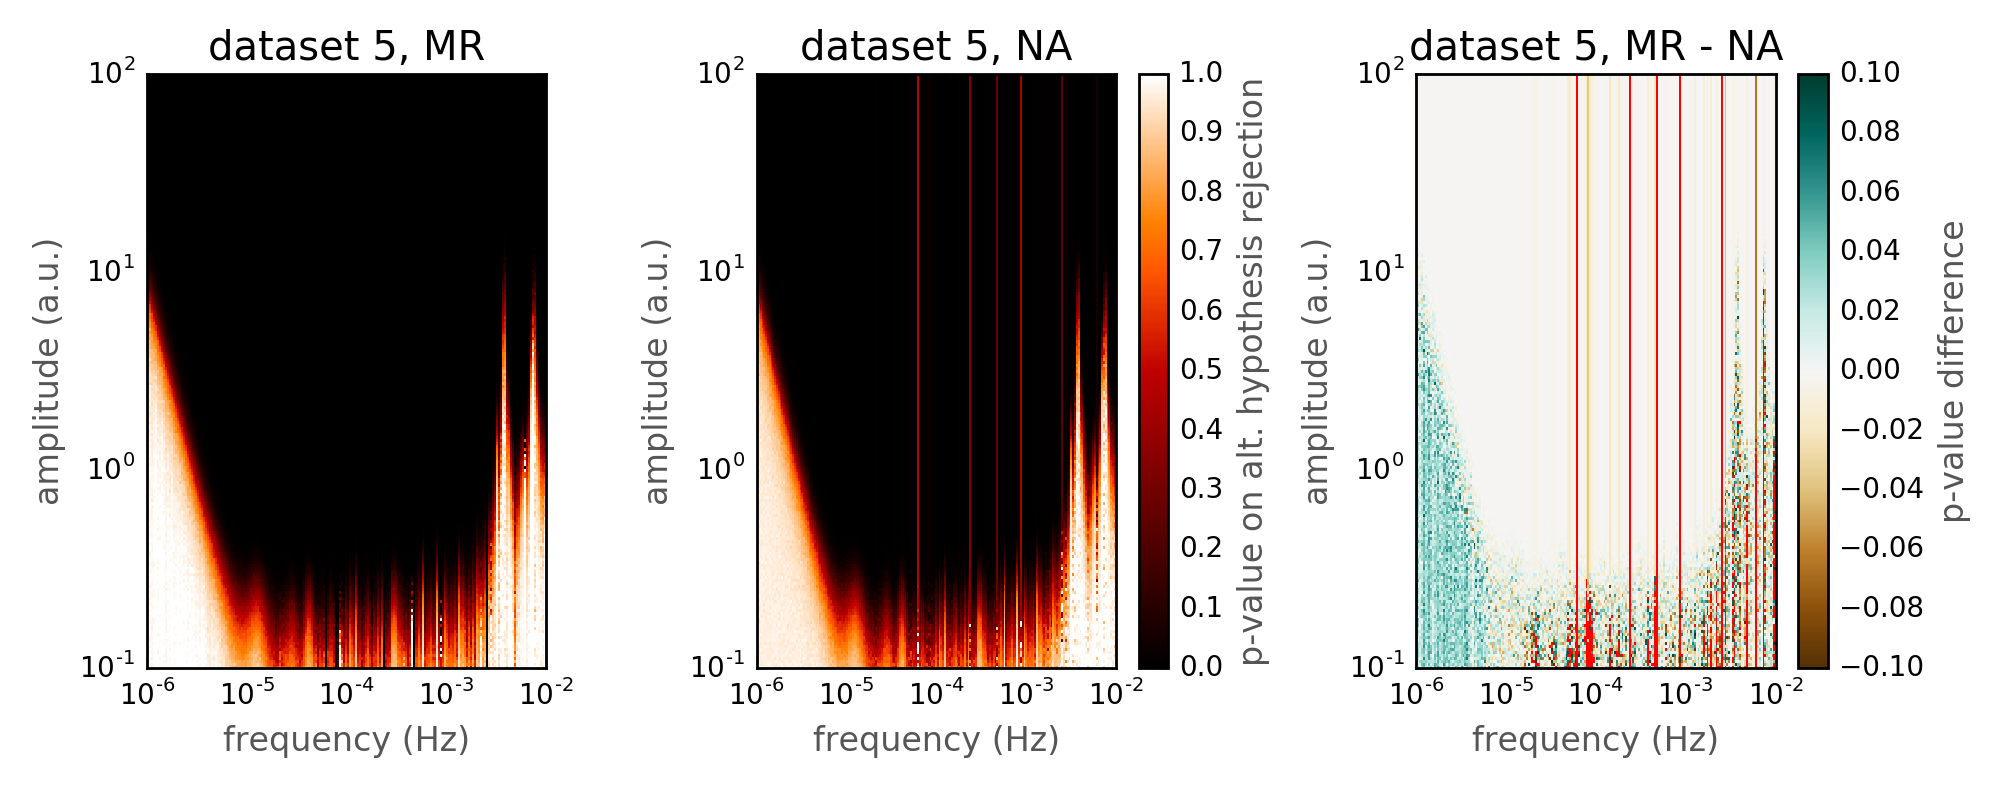
\includegraphics[width=0.45\linewidth]{gfx/axions/comparison/comparison_exclusion_dataset5.png}
  \centering 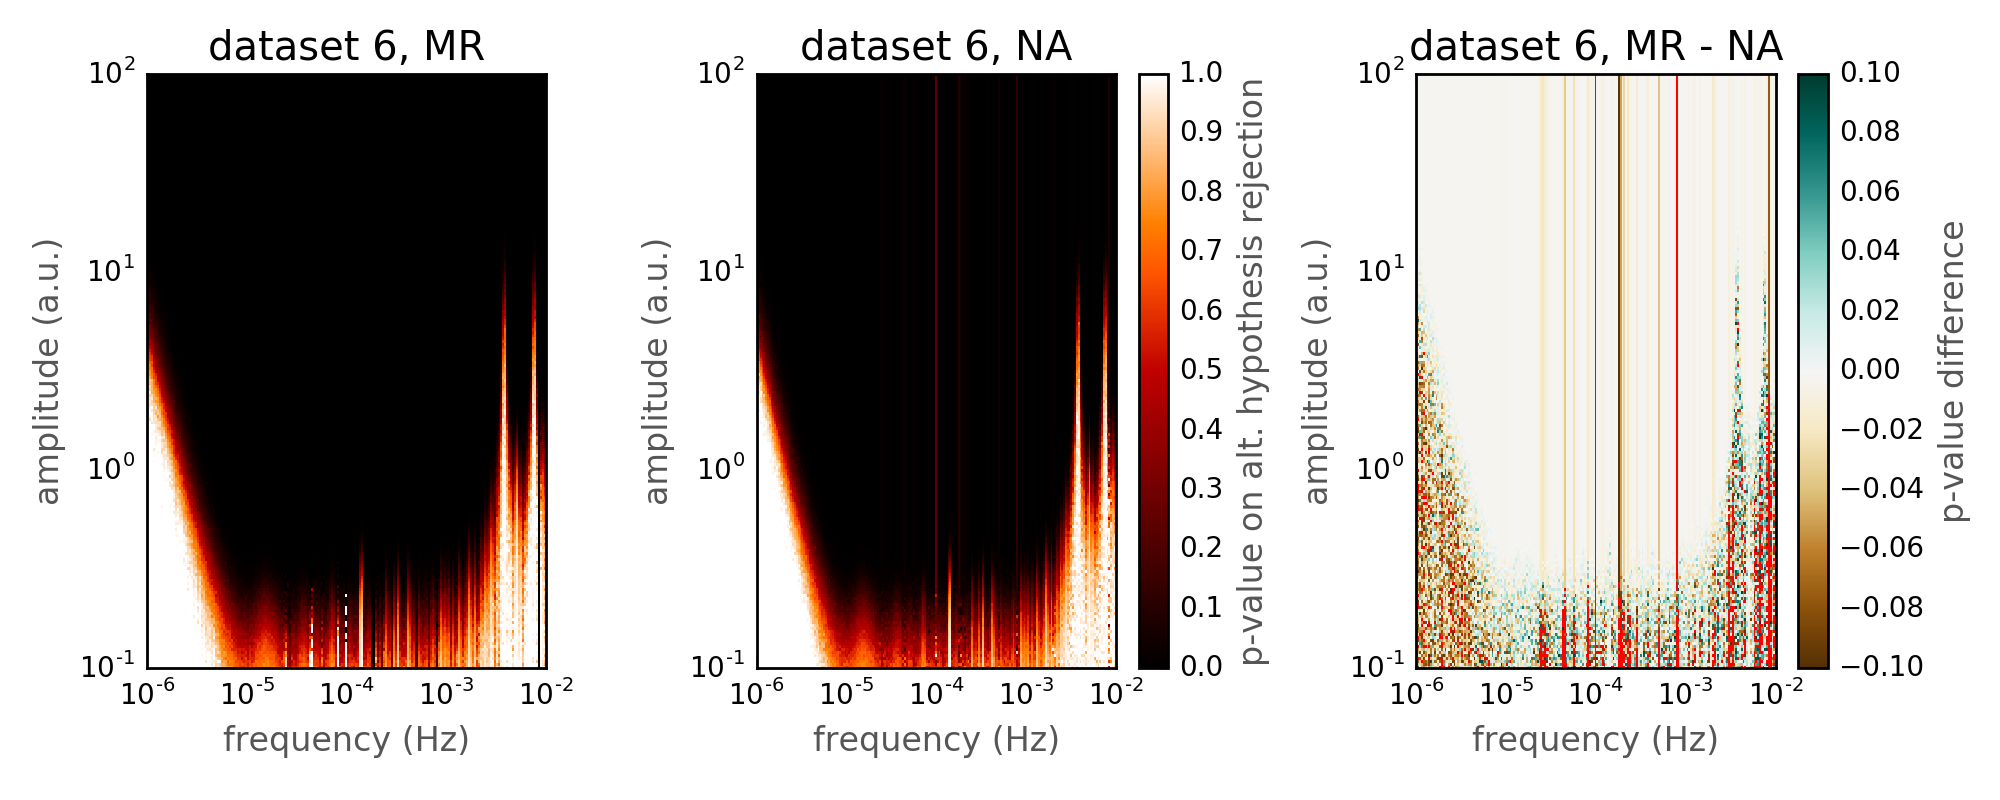
\includegraphics[width=0.45\linewidth]{gfx/axions/comparison/comparison_exclusion_dataset6.png}
  \centering 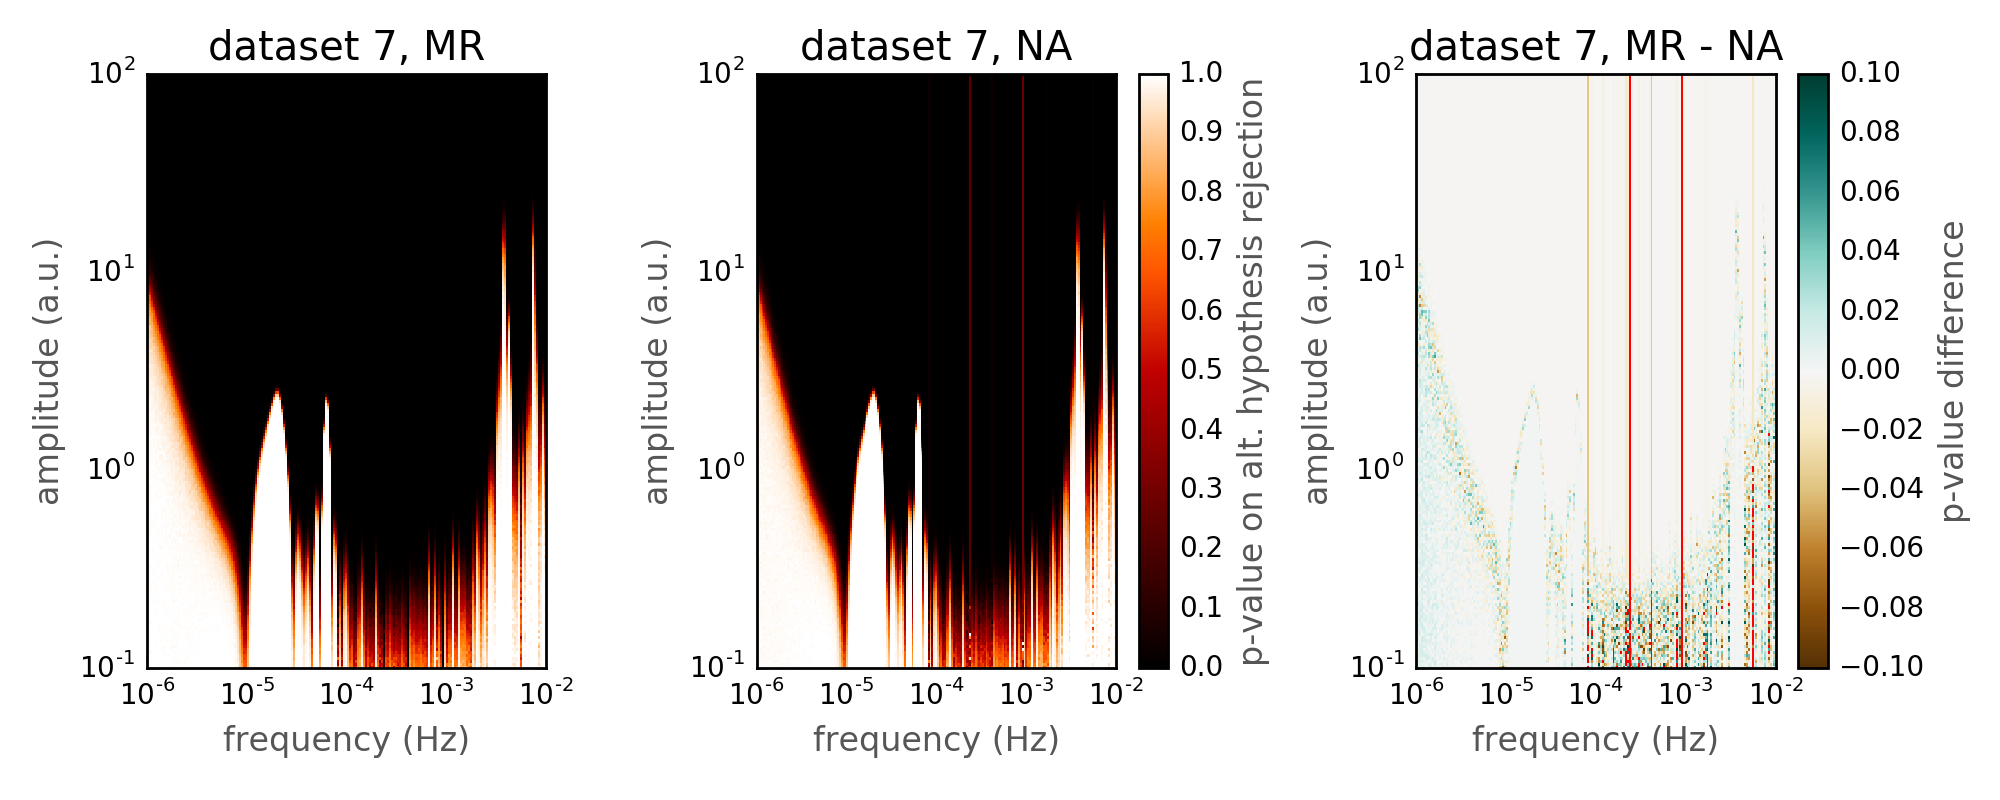
\includegraphics[width=0.45\linewidth]{gfx/axions/comparison/comparison_exclusion_dataset7.png}
  \centering 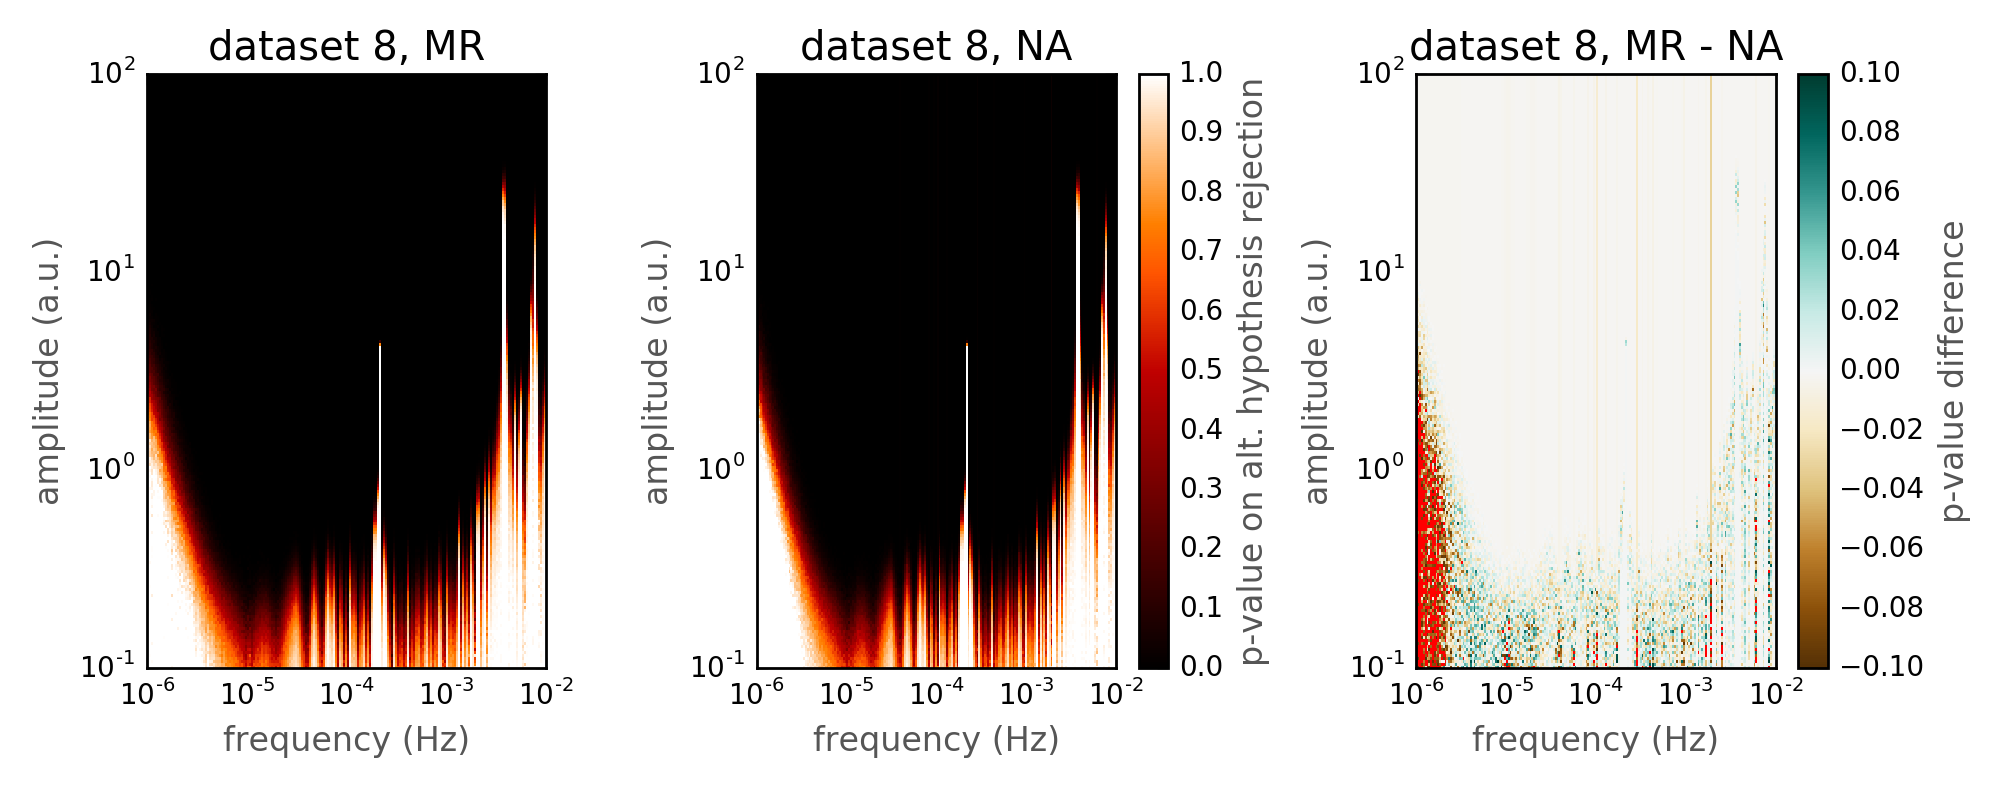
\includegraphics[width=0.45\linewidth]{gfx/axions/comparison/comparison_exclusion_dataset8.png}
  \centering 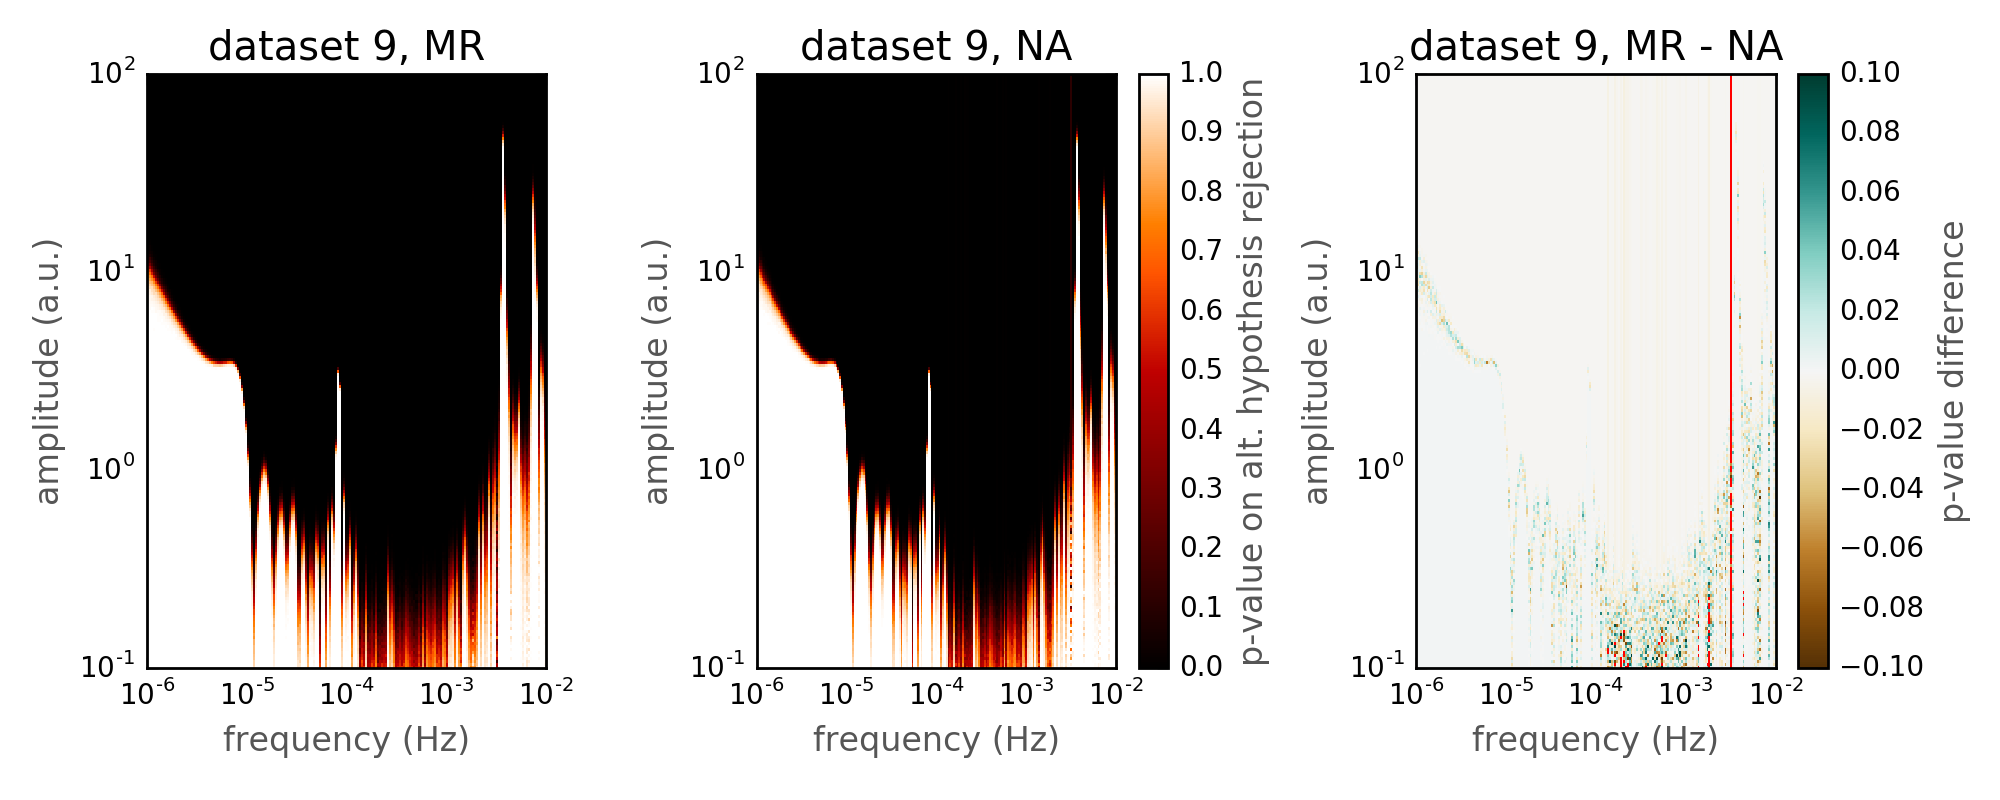
\includegraphics[width=0.45\linewidth]{gfx/axions/comparison/comparison_exclusion_dataset9.png}
  \caption{Comparison between the analysis implemented by Nicholas Ayres (NA) and Michal  Rawlik (MR). This figure presents the \emph{exclusion} part of the analysis. For each fake dataset three maps in the signal parameter space (frequency--amplitude) are shown. From left to right: (a) p--value on exclusion as calculated by Michał Rawlik (MR), (b) p--value on exclusion as calculated by Nicholas Ayres (NA), (c) the difference of the two. Differences larger then 0.1 are marked red.}
  \label{fig:comparison_exclusion}
\end{figure*}

\section{Derivation of what we measure with R}
\label{Sec:R_derivation}

\begin{align}
H &= - \boldsymbol{\mu} \cdot \mathbf{B} - \mathbf{d} \cdot \mathbf{E} \\
h \nu &= 2 \left( \boldsymbol{\mu} \cdot \mathbf{B} \pm \mathbf{d} \cdot \mathbf{E} \right) = 2 \left(\mu B \pm d E \right) \\
R &= \frac{\nu_n}{\nu_{Hg}} = \frac{ \frac{2}{h} \left( \mu_n B + d_n E \right) }{ \frac{2}{h} \left( \mu_{Hg} B + d_{Hg} E \right) } = \nonumber \\
    &= \frac{ \left( \mu_n B \pm d_n E \right) }{ \left( \mu_{Hg} B \pm d_{Hg} E \right) } = \nonumber \\
    &= \frac{ \mu_n B }{ \left( \mu_{Hg} B \pm d_{Hg} E \right) } \pm \frac{ d_n E }{ \left( \mu_{Hg} B \pm d_{Hg} E \right) } = \nonumber \\
    &= \frac{\mu_n}{\mu_{Hg}} \cdot \frac{1}{ 1 \pm \frac{d_{Hg} E}{\mu_{Hg} B}} \pm \frac{d_n E}{\mu_{Hg} B} \cdot \frac{1}{1 \pm \frac{ d_{Hg}E }{ \mu_{Hg} B}} = \nonumber \\
    &= \left\{ \frac{1}{1 \pm x} = 1 \mp x \right\} = \nonumber \\
    &= \frac{\mu_n}{\mu_{Hg}} \mp d_{Hg} \frac{\mu_n}{\mu_{Hg}} \frac{E}{\mu_{Hg} B} \pm d_n \frac{E}{\mu_{Hg} B} \mp d_n d_{Hg} \left( \frac{E}{\mu_{Hg} B} \right)^2 \\
\delta R &\approx \left( d_n \mp  d_{Hg} \frac{\mu_n}{\mu_{Hg}} \right) \frac{E}{\mu_{Hg} B} = \left\{ \boldsymbol{\mu} = \gamma \mathbf{S} \right\} \nonumber \\
   & = \left( d_n \mp  d_{Hg} \frac{\gamma_n}{\gamma_{Hg}} \right) \frac{2 E}{\gamma_{Hg} h B}
\end{align}


\section{END Below is the everything document about the axion search}





\section{START The PRX paper}


\section{Introduction}
\label{Sec:Introduction}
% \textbf{Introduction.} ---
%\note{Text formatted like this are notes and comments, not part of the final text.}

%\note{GP, TL, DR: Earlier searches for oscillating signals using our apparatus should be mentioned and cited.
%namely:
%24h modulation of R: I. Altarev et al Phys.Rev.Lett. 103 (2009) 081602
%12h and 24h modulation of nEDM: I. Altarev et al. Europhys.Lett. 92 (2010) 51001}
% \note{KK: Comment explicitly on the phase of the signal being random in the simulations. We are not looking at the worst case scenario!}
%\note{MMM: I would recommend subdividing your paper into labeled sections for the benefit of the reader.}
%\note{MR: PRL papers have no sections, right?}
%\note{YS: PRL letters are not allowed to have the usual sections (like in the other subdivisions of Physical Review), but it is possible to have small subheadings throughout the text, if this would help:~e.g., \textbf{Introduction.} --- Text ...}

%\note{YS: In the list of references, footnote [18] appears to have been duplicated in [66]. Is it possible to have the footnote appear only once in the references (as [18]), like we had before?}
%note{MR: Note. \footnotemark does the trick.}

% \note{KK: Remove the title from Ref. [15].}

% \note{YS: In Ref.~[81], remove ''[On-line; accessed date]'', and replace by url.}

Astrophysical and cosmological observations indicate that $26 \%$ of the total energy density and $84 \%$ of the total matter content of the Universe is dark matter (DM) \cite{Planck2015}, %\note{FP: Right at the beginning you say there is 85\% dark matter - normally its stated that there is 27\% DM and 68\% Dark Energy - can you just add this up to one number?} \note{PSW: I wouldn't sum over dark matter and dark energy. Both have different observational indicators and interpretations.} \note{Doddy: Reword to "26\% of the total energy density of the Universe, and 84\% of the total matter content"} \note{YS: I agree with Doddy's suggestion.},
the identity and properties of which still remain a mystery.
One of the leading candidates for cold DM
%\note{PMM: \ldots candidate for cold dark matter. cite: Phys. Rev. Lett. 108, 061304 also. Axion being hot dark matter needs more exotic interactions.}
%\note{YS: The general consensus in cosmology is that the vast majority of DM should be cold, so the term DM without qualifiers is often taken to be synonymous with cold DM. Hot DM is quite exotic (the axion is no exception). On a side note, the mentioned paper refers to the formation of an axion BEC with an enormous correlation length (much larger than the standard assumption of the de Broglie wavelength associated with the virialised component of the axions) - this is quite a contraversial claim, which is disputed by a sizeable portion of the physics community.}
is the axion, a pseudoscalar particle which was originally hypothesised to resolve the strong CP problem of quantum chromodynamics (QCD) \cite{PQ1977A,PQ1977B,Weinberg1978,Wilczek1978,Kim1979,Zakharov1980,Zhitnitsky1980A,*Zhitnitsky1980B,Srednicki1981}.
Apart from the canonical QCD axion, various axion-like particles have also been proposed, for example in string compactification models \cite{Witten1984,Conlon2006,Witten2006,Arvanitaki2010,Arias2012,Marsh2015Review}.

Low-mass ($m_a \lesssim 0.1~\textrm{eV}/c^2$) axions can be produced efficiently via non-thermal production mechanisms, such as vacuum misalignment \cite{Preskill1983cosmo,Sikivie1983cosmo,Dine1983cosmo} in the early Universe, and subsequently form a coherently oscillating classical field \footnote{Although non-thermal production mechanisms typically impart negligible kinetic energy to the produced axions, the gravitational interactions between axions and ordinary matter during galactic structure formation subsequently virialise galactic axions ($v_{\textrm{vir}}^{\textrm{local}} \sim 300$~km/s), giving an oscillating galactic axion field the finite coherence time:~$\tau_{\textrm{coh}} \sim 2\pi / m_a v_{\textrm{vir}}^2 \sim 2\pi \cdot 10^6 / m_a $, i.e., $\Delta \omega / \omega \sim 10^{-6}$. }:~$a = a_0 \cos(\omega t)$, with the angular frequency of oscillation given by $\omega \approx m_a c^2 / \hbar$, where $m_a$ is the axion mass (henceforth, we shall adopt the units $\hbar = c = 1$).
%\note{PMM: replace with ...classical field - a, $a=a_0 cos(wt)$, with the angular frequency of oscillations given by $\omega \sim m_a$, where $m_a$ is the axion mass.
%No need to mention $c=\hbar = 1$ as you've already used natural units before. Maybe you can mention in brackets: ... $\omega \sim m_a$ (in natural units). This is the first time $m_a$ is used so needs to be explicitly mentioned as the axion mass.}
The oscillating axion field carries the energy density $\rho_a \approx m_a^2 a_0^2 /2$. Due to its effects on structure formation \cite{Khlopov1985}, ultra-low-mass axion DM in the mass range $10^{-24}~\textrm{eV} \lesssim m_a \lesssim 10^{-20}$ eV has been proposed as a DM candidate that is observationally distinct from, and possibly favourable to, archetypal cold DM \cite{Hu2000,Marsh2014,Schive2014,Marsh2015Review,Hui2017}.
The requirement that the axion de Broglie wavelength does not exceed the DM size of the smallest dwarf galaxies and consistency with observed structure formation \cite{Marsh2015B,Schive2015,Marsh2017} give the lower axion mass bound $m_a \gtrsim 10^{-22}$ eV, if axions comprise all of the DM. However, axions with smaller masses can constitute a sub-dominant fraction of DM~\cite{Hlozek15}.

It is reasonable to expect that axions interact non-gravitationally with standard-model particles.
Direct searches for axions have thus far focused mainly on their coupling to the photon (see the review \cite{Axion-Review2015} and references therein).
% **WHY WAS THIS HERE?  (MALCOLM)** coherently oscillating spin-dependent effects due to the
%\note{BL: We should cite: The here described experiment obtained a new limit on axion-like particles using ultracold neutrons \cite{Afach2015Exotic}.}
%\note{YS: In the earlier (long) version of this paper, we actually had a reference to this paper and several other papers on related applications of ultracold neutrons to look for new physics. In the process of shortening the paper, the paragraph containing these references was cut out, but perhaps we could restore the references somewhere in the paper.}
Recently, however, it has been proposed to search for the interactions of the coherently oscillating axion DM field with gluons and fermions, which can induce oscillating electric dipole moments (EDMs) of nucleons \cite{Graham2011} and atoms \cite{Stadnik2014A,Roberts2014A,Roberts2014B}, and anomalous spin-precession effects \cite{Flambaum2013Patras,Stadnik2014A,Graham2013}.
The frequency of these oscillating effects is dictated by the axion mass, and more importantly, these effects scale linearly in a small interaction constant \cite{Graham2011,Stadnik2014A,Roberts2014A,Roberts2014B,Flambaum2013Patras,Graham2013}, whereas in previous axion searches, the sought effects scaled quadratically or quartically in the interaction constant \cite{Axion-Review2015}.
%\note{PMM: needs citation, even if repeated with [27-31]}

In the present work, we focus on the axion-gluon and axion-nucleon couplings:
\begin{align}
\label{Axion_couplings}
\mathcal{L}_{\textrm{int}} = \frac{C_G}{f_a} \frac{g^2}{32\pi^2} a G^{b}_{\mu \nu} \tilde{G}^{b \mu \nu}  - \frac{C_N}{2f_a} \partial_\mu a ~ \bar{N} \gamma^\mu \gamma^5 N \, ,
\end{align}
where $G$ and $\tilde{G}$ are the gluonic field tensor and its dual, $b=1,2,...,8$ is the  color index, $g^2 / 4 \pi$ is the color coupling constant, {\color{black}$N$ and $\bar{N} = N^\dagger \gamma^0$ are the nucleon field and its Dirac adjoint,} $f_a$ is the axion decay constant, and $C_G$ and {\color{black}$C_N$} are model-dependent dimensionless parameters.
Astrophysical constraints on the axion-gluon coupling in (\ref{Axion_couplings}) come from Big Bang nucleosynthesis \cite{Blum2014,StadnikThesis,Stadnik2015D}:~$m_a^{1/4} f_a / C_G \gtrsim 10^{10}~\textrm{GeV}^{5/4}$ for $m_a \ll 10^{-16}~\textrm{eV}$ and $m_a f_a / C_G \gtrsim 10^{-9}~\textrm{GeV}^{2}$ for $m_a \gg 10^{-16}~\textrm{eV}$, assuming that axions saturate the present-day DM energy density, %$\bar{\rho}_\textrm{DM} = 1.3 \times 10^{-6}~\textrm{GeV/cm}^3$ \cite{Planck2015},
%\note{Maurits: I see that the dark matter energy density that is used on page 1 of the paper (1.3x10-6 GeV/cc) is very different than the number I normally come across (0.3 GeV/cc) for the direct DM searches. The paper does refer to the local DM density of 0.4 GeV/cc on the next page, but in the reference [1] I cannot find this number of 1.3x10-6GeV/cc. It could be that I overlooked something, as it is a rather chunky Planck collaboration paper that ref[1] refers to, but am I missing something?}
%\note{YS: These numbers refer to different things. The number $1.3 \times 10^{-6}$ GeV/cc refers to the present-day DM energy density that is averaged over the scale of the observable Universe, while the number 0.4 GeV/cc refers to the DM energy density in our local galactic region (which is averaged over a much smaller length scale of only about 0.1 - 1 kpc). Basically, the density of DM is much higher inside galaxies than it is outside of galaxies.}
%\note{GP, TL, DR: To calculate a limit on the Axionlike coupling strength from the limit on the oscillation amplitude of EDM one needs the local dark matter energy density.
%There is a debate in the dark matter literature on this value which is poorly known, however all dark matter experiments report limits using the "standard" value rho = 0.3 $GeV/cm^3$.
%See for example the latest Xenon1T paper arXiv:1705.06655v2
%I suggest we use the standard value instead of 0.4 $GeV/cm^3$. }
%\note{YS: The current Particle Data Group review on DM quotes the value $\rho \approx 0.4~\textrm{GeV/cm}^{3}$.
%I am told by other physicists that recent values of $\rho$ have hovered in the range $0.3 - 0.45~\textrm{GeV/cm}^{3}$, while older values in the literature hovered in the wider range $0.2 - 0.8~\textrm{GeV/cm}^{3}$. In either case, I do not know why the value $0.3~\textrm{GeV/cm}^{3}$ is quoted so frequently in experimental papers, since it lies towards the lower end of these ranges in both cases (even though we know, from consideration of the planetary orbits within our Solar System, that $\rho$ can be many orders of magnitude larger inside our Solar System than the local galactic average).}
and from supernova energy-loss bounds \cite{Graham2013,Raffelt1990Review}:~$f_a / C_G \gtrsim 10^6 ~\textrm{GeV}$ for $m_a \lesssim 3 \times 10^{7}~\textrm{eV}$.
{\color{black}Astrophysical constraints on the axion-nucleon coupling in (\ref{Axion_couplings}) come from supernova energy-loss bounds \cite{Raffelt1990Review,Raffelt2008LNP}:~$f_a / C_N \gtrsim 10^9 ~\textrm{GeV}$ for $m_a \lesssim 3 \times 10^{7}~\textrm{eV}$, while existing laboratory constraints come from magnetometry searches for new spin-dependent forces mediated by axion exchange \cite{Romalis2009_NF}:~$f_a / C_N \gtrsim 1 \times 10^4 ~\textrm{GeV}$ for $m_a \lesssim 10^{-7}~\textrm{eV}$. }


The axion-gluon coupling in (\ref{Axion_couplings}) induces the following oscillating EDM of the neutron via a chirally-enhanced 1-loop process~%\footnote{Interaction (\ref{Axion_couplings}) also non-perturbatively induces a mass $m_a \approx 6C_G\,\mu\text{eV} \cdot (10^{12}\text{ GeV}/f_a)$.
%Axions with masses much smaller than this are theoretically fine-tuned.}
\cite{tuningfootnote,Witten1979,*Witten1979B,Pospelov1999}:
%\note{KK: merge to [42-44]}
\begin{equation}
\label{eq:nEDM_axion}
d_\mathrm{n}(t) \approx +2.4 \times 10^{-16} ~ \frac{C_G a_0}{f_a} \cos(m_a t) ~ e \cdot \textrm{cm} \, .
\end{equation}
The axion-gluon coupling in (\ref{Axion_couplings}) also induces oscillating EDMs of atoms via the 1-loop-level oscillating nucleon EDMs and tree-level oscillating P,~T-violating intranuclear forces (which give the dominant contribution) \cite{Stadnik2014A,Flambaum1984EDM,*Flambaum1984EDMB}.
In the case of $^{199}$Hg, the oscillating atomic EDM is \cite{Stadnik2014A,StadnikThesis,Flambaum1985EDM,Flambaum1985EDMB,Flambaum2002EDM,Dmitriev2003A,Dmitriev2003B,Dmitriev2005,Engel2005,Engel2010}:
\begin{equation}
\label{199Hg-EDM_axion}
d_{\textrm{Hg}}(t) \approx +1.3 \times 10^{-19} ~ \frac{C_G a_0}{f_a} \cos(m_a t) ~ e \cdot \textrm{cm} \, ,
\end{equation}
which is suppressed compared to the value for a free neutron (\ref{eq:nEDM_axion}), as a consequence of the Schiff screening theorem for neutral atoms \cite{Schiff1963}.
%\note{KK: a question to our theory friends: Eqns. (2) and (3) suggest that $d_n$ and $d_\textrm{Hg}$ would have the same sign. Is this intended or are we rather talking about the modulus?}
%\note{YS: Yes, the same signs for $d_n$ and $d_\textrm{Hg}$ are intended here.}
%\note{MR: Should we explicitly point that out then?}
%\note{YS: I think this would be a good idea. We could explicitly add "+" signs in both Eqs. (2) and (3) to remove any ambiguity.}
%\note{CG: Might be good to comment that the Hg contribution is quite safely assumed to be negligible compared to the neutron for the purposes of this paper.}
The amplitude of the axion DM field, $a_0$, is fixed by the relation $\rho_a \approx m_a^2 a_0^2 /2$.
In the present work, we assume that axions saturate the local cold DM energy density $\rho_{\mathrm{DM}}^{\mathrm{local}} \approx 0.4~\textrm{GeV/cm}^3$ \cite{Catena2010}.




%Crucially, the constant amplitude of the axion DM field, $a_0$, is fixed by the known DM density at the location of the Earth, $\rho_{\mathrm{DM}}=\approx 0.4~\textrm{GeV/cm}^3$ \cite{Catena2010} (when reporting constraints on the couplings we assume axions make up all the local DM).


% Our experiment is also sensitive to the time-dependent energy shifts induced by the derivative coupling of an oscillating galactic axion DM field, $a = a_0 \cos(m_a t - \vtr{p}_a \cdot \vtr{r})$, with spin-polarised nucleons in (\ref{Axion_couplings}):
The derivative coupling of an oscillating galactic axion DM field, $a = a_0 \cos(m_a t - \vtr{p}_a \cdot \vtr{r})$, with spin-polarized nucleons in (\ref{Axion_couplings}) induces time-dependent energy shifts according to:
\begin{equation}
\label{potential_axion-wind}
H_{\textrm{int}} (t) = \frac{C_N a_0}{2 f_a} \sin(m_a t) ~ \vtr{\sigma}_N \cdot \vtr{p}_a \, .
\end{equation}
The term $\vtr{\sigma}_N \cdot \vtr{p}_a$ is conveniently expressed by transforming to a non-rotating celestial coordinate system (see, e.g., \cite{Kostelecky1999}):
\begin{align}
\label{sigma-p_a_2}
\vtr{\sigma}_N \cdot \vtr{p}_a  &= \hat{m}_F f(\sigma_N) m_a |\vtr{v}_a|  \notag \\
& \times \left[\cos(\chi) \sin(\delta) + \sin(\chi) \cos(\delta) \cos(\Omega_{\textrm{sid}} t - \eta) \right] \, ,
\end{align}
where $\chi$ is the angle between Earth's axis of rotation and the spin quantization axis ($\chi = 42.5 ^\circ$ at the location of the PSI), $\delta \approx -48 ^\circ$ and $\eta \approx 138 ^\circ$ are the declination and right ascension of the galactic axion DM flux relative to the Solar System \cite{NASA2014web}, $\Omega_{\textrm{sid}} \approx 7.29 \times 10^{-5}~\textrm{s}^{-1}$ is the daily sidereal angular frequency, $\hat{m}_F = m_F / F$ is the normalized projection of the total angular momentum onto the quantization axis, and $f(\sigma_N) = +1$ for the free neutron, while $f(\sigma_N) = -1/3$ for the $^{199}$Hg atom in the Schmidt (single-particle) model.


Here, we report on a search for an axion-induced oscillating EDM of the neutron (nEDM) based on an analysis of the ratio of the spin-precession frequencies of stored ultracold neutrons and $^{199}$Hg atoms, which is a system that had previously also been used as a sensitive probe of new non-EDM physics \cite{Altarev2009,Altarev2010,Afach2015_NF}.
We divided our analysis into two parts.
We first analyzed the Sussex--RAL--ILL nEDM experiment data \cite{Baker2014}, covering oscillation periods longer than days (\emph{long time--base}).
Then we extended the analysis to the data of the PSI nEDM experiment \cite{Baker2011}, which allowed us to probe oscillation periods down to minutes (\emph{short time--base}).
Our analysis places the first laboratory constraints on the axion-gluon coupling.
We also report on a search for an axion-wind spin-precession effect, using the data of the PSI nEDM experiment. Our analysis places the first laboratory constraints on the axion-nucleon coupling from the consideration of an effect that is linear in the interaction constant.

\section{Long time-base analysis}
The Sussex--RAL--ILL room temperature nEDM experiment ran from 1998 to 2002 at the PF2 beamline at the Institut Laue-Langevin (ILL) in Grenoble, France.
This experiment set the current world-best limit on the permanent time-independent neutron EDM, published in 2006 \cite{Baker2006, *Baker2006B}. The data were subsequently reanalyzed to give a revised limit in 2015 \cite{Pendlebury2015}. The technical details of the apparatus are described in full in \cite{Baker2014}, but we summarize the main experimental details here for the reader.

The experiment was based on Ramsey interferometry \cite{Ramsey1950} of ultracold neutrons \cite{UCN-Review1979,UCN-Review1994}.
%\note{CG: Might be good to define UCN or at least give a reference.}
The neutrons were stored in parallel or antiparallel electric and magnetic fields, where their Larmor precession frequency is given by
\begin{equation}
  \label{eq:Larmor}
  h\nu_\mathrm{n} = 2 \left| \mu_\mathrm{n} B \pm d_\mathrm{n} E \right| \, ,
\end{equation}
%\note{EW: I might be misremembering conventions, but shouldn’t the $n$ in $d_n$ and $mu_n$ be roman instead of italic? Same for the subscript a for axion? Or is the subscript a referring to the classical field a (in which case it should be italic)?}
%\note{YS: I don't think there's a standard convention on this. I've seen both italicised and Roman variants for elementary-particle subscripts in the literature. As long as we're consistent, then it shouldn't matter which convention we use.}
with the sign depending on the field configuration.
$E$ and $B$ are the magnitudes of the electric and magnetic fields, respectively.
By measuring the frequency difference between the two field configurations, a value for the neutron EDM, $d_\mathrm{n}$, was inferred.

%\note{PH: An irritant from the language perspective is the use of the "historic present" -- the measurement "is" rather than "was" conducted, and so on.}
%\note{PSW: I support PH remark, and would prefer a description of the experimental and analysis procedures in simple past (was instead of is).}
The measurement was conducted in a series of \emph{cycles}, each approximately 5 minutes long. A cycle began with a filling of neutrons polarized along the fields into the precession chamber from the ultracold neutron source~\cite{Steyerl1986}.
% \note{CG: Unclear to the reader what "the source" refers to.}
% Once they were within the chamber, an oscillating $\pi/2$ pulse \note{PSW: In general these pulses are far off from pi/2. May be call it a spin-tip pulse.} lasting 2 seconds was applied to begin the precession. Simultaneously, a population of polarized $^{199}$Hg atoms was released into the chamber, and a rotating $\pi/2$ pulse was also applied to set these atoms into free precession. The particles were stored and allowed to precess freely for 130 seconds. After this, the neutrons were subjected to a second $\pi/2$ analysing pulse.
Once they are in the chamber, enclosed from top and bottom with electrodes, a \unit[29]{Hz} NMR pulse lasting 2 seconds was applied to rotate the neutron spins into the transverse plane of the electromagnetic fields where they began to precess. Prior to the pulse, a population of polarized $^{199}$Hg atoms was released into the chamber, another 2-second \unit[29]{Hz} pulse, in-phase with the first one, was applied.
% d an \unit[8]{Hz} NMR pulse was applied to set these atomsorientation free precession. The particles were stored and allowed to precess freely for 130 seconds. After this, the neutron spins were rotated back into the longitudinal plane by a second \unit[29]{Hz} pulse.
%(ILL) or 180 seconds (PSI) \note{MR: not mention PSI here?}.
% \note{GP, TL, DR: "simultaneously, a population of polarized 199Hg atoms is released..." -> "Prior to the pi/2 pulse, a population...", "precess freely for 130 s" -> it is in fact 180s for the PSI data. }
%\note{FP: you call the second pi/2-pulse "analysing pulse". I guess this is somehow confusing (and maybe formally not correct), especially since one line afterwards you mention the "analyzing foil"}.
The neutrons were then emptied into a detector through a spin-analyzing foil. Over 1--2 days, many of these cycles were performed. The electric field's polarization was reversed every hour. We term one continuous block of data taking in the same magnetic-field configuration, but including both directions of electric field, a \emph{run}. One run gives a $d_\mathrm{n}$ estimate.
%\note{MR: This would be the place to mention the crossing lines, if we want it. Maybe a short comment about the one-run ILL $d_n$ estimate would be in place. Does it still include systematic effects? Or does it not? Later, we say that we assume zero offset in fit, it may need a little motivation.}

In order to suppress cycle--to--cycle changes in the magnetic field, the analysis was performed on the ratio of the neutron and mercury precession frequencies $R$, which, using (\ref{eq:Larmor}), is \cite{Baker2014}:
\begin{align}
  \label{eq:R}
  % R &= \frac{\nu_n}{\nu_{Hg}} = \frac{\mu_n}{\mu_{Hg}} \pm \left( d_n - \frac{\mu_n}{\mu_{Hg}} \, d_{Hg} \right) \frac{E}{\mu_{Hg} B} + \mathcal{O}(d^2) \ ,
  R &\equiv \frac{\nu_\mathrm{n}}{\nu_\textrm{Hg}} = \frac{\mu_\mathrm{n}}{\mu_\textrm{Hg}} \pm \left( d_\mathrm{n} - \frac{\mu_\mathrm{n}}{\mu_\textrm{Hg}} \, d_\textrm{Hg} \right) \frac{2 E}{ h  \nu_\textrm{Hg}} + \Delta \, ,
\end{align}
where the signs correspond to parallel and antiparallel field configurations. $\Delta$ encapsulates all higher-order terms and systematic effects, which are corrected for when a run is analyzed~\cite{Pendlebury2015}.
% \note{FP: what is the $d^2$ in the higher order term of the equation - is it a dipole moment? But then it has no index (n or Hg), if it's something else it is not explained I guess.}
% \note{MR: We need $\mathcal{O}(d^2)$, as there are terms $\propto d_n^2$, $\propto d_{Hg}^2$, and $\propto d_n d_{Hg}$. Will need to clarify that in words, I can't come up with a sensible notation.}
% \note{PSW: You do not only have corrections of higher order of electric-dipole signals but also due to the different adiabatic regimes. Try to find a better way of generalizing higher order terms.}
This analysis is sensitive to oscillations in the quantity $d_\mathrm{n} - \left( \mu_\mathrm{n} / \mu_\textrm{Hg} \right) \, d_\textrm{Hg}$, with $\mu_\mathrm{n} / \mu_\textrm{Hg} = -3.8424574(30)$~\cite{Afach2014magmoment}.

%, which we conveniently give in $\unit[10^{-26}]{e \cdot cm}$ units. %\note{MR: Need to give the magnetic field strength ($B$ in the above equation) used for the $R$ to $d_n$ conversion. For the PSI analysis is taken to be $\unit[1.03536]{\upmu T}$.}
% \note{EW: I think equation 5 is incomplete. In principle it should also include all systematic effects influencing R, such as
% - rotation of the earth
% - $<Bt^2>$
% - Linear and cubic GPE in fHg/fn
% - HgM light shift
% - Shift due to gravity (G1,0 and G3,0 mainly, others as well)
% - …?
% Seeing that most of them aren’t really relevant to the story, maybe you can condense them into a delta or something? But I think you should at least mention the shift due to gravity, as this one reappears a bit later in the paper. (And you mention the crossing lines procedure as well.)}
% \note{YS: Maybe could introduce $\Delta$ as the last term in (5), defined as ``all higher-order terms and systematic effects (such as the slight downwards displacement of the ultracold neutrons with respect to the hot cohabitating mercury atoms'' [Give a reference here?])?}

In our analysis, we were looking for an oscillating EDM. We performed this search in frequency space by evaluating \emph{periodograms} -- estimators of the power spectrum. An oscillation in the time domain would show up as an excess in the power (or, equivalently, amplitude) relative to the expected distribution due to experimental noise.

In the case of the long time--base analysis, we considered the time series of $d_\mathrm{n}$ measurements from individual runs (after having corrected for the ``False EDM'' effect \cite{Pendlebury2004} using the crossing lines procedure \cite{Pendlebury2015}). %\note{NA: mention crossing lines here, because it doesn't make sense until you explain that you use the R rather than $\nu_{n}$},
The measurements are neither evenly spaced nor have equal uncertainties.
%To calculate the periodogram of the data series, we use the Least Squares Spectral Analysis (LSSA) \cite{Scargle1982,Cumming2004}, where the amplitude at frequency $f$ is estimated by the amplitude of the best fit oscillation of that frequency. We evaluate the periodogram at a set of 1334 \note{@NA todo double check} trial frequencies, evenly spaced between 0 (exclusive) and $\unit[10]{\upmu Hz}$ \note{@Nick verify}. The spacing, $\unit[7.49]{nHz}$, is chosen to be equal to the intrinsic spectral resolution of the dataset (its inverse time span).
%An axion DM signal (with expected coherence set by $\Delta \omega/ \omega \sim 10^{-6}$) is narrower than the spectral resolution in the whole range of tested frequencies. The width of a signal peak is thus set by the spectral resolution, which we choose to be the spacing of the trial frequencies.
%By doing so, we ensure that we do not miss a DM signal in the entire considered frequency range.
To calculate the periodogram of the data series, we used the Least Squares Spectral Analysis (LSSA) method \cite{Scargle1982,Cumming2004}, where the amplitude at frequency $f$ was estimated by the amplitude of the best fit oscillation of that frequency. We evaluated the periodogram at a set of 1334 trial frequencies, evenly spaced between \unit[100]{pHz} (arbitrarily chosen, a period of about 300 years, much longer than the four--year span of the data set) and $\unit[10]{\upmu Hz}$ (a period of about a day, the time it typically took to get one $d_\mathrm{n}$ estimate).
An axion DM signal, with expected coherence set by $\Delta f \sim 10^{-6} f~$\footnotemark[1],
% \note{PH: not clear where it's from.} \note{YS: Added a reference to the existing footnote to clarify this point.}
is narrower than the spectral resolution ($\unit[7.49]{nHz}$, the inverse span of the data set) in the whole range of frequencies we were sensitive to.
% \note{FP: This is a bit confusing to me since you compare relative with absolute resolution. Can you maybe in addition translate the \unit[7.5]{nHz} to a relative resolution.}
% \note{MR: The key is \emph{the whole range of frequencies}; the relative relation holds in the whole range. Formulate better.}
% \note{YS: Maybe we could rewrite $\Delta f/ f \sim 10^{-6}$ as $\Delta f \sim 10^{-6} f$ above?}
% The width of a signal peak is thus set by the spectral resolution, which we chose to be the spacing of the trial frequencies. We evaluated the periodogram at a set of 1334 trial frequencies, evenly spaced between \unit[100]{pHz} (arbitrary chosen, a period of about 300 years, much longer than the span of the data set) and \unit[10]{\upmu Hz} (a period of about a day, the minimal separation between  $d_n$ estimation in the ILL experiment).
%evenly spaced between $\unit[100]{pHz}$ (arbitrarily chosen) and $\unit[10]{\upmu Hz}$.
% \note{MMM: Was 10 uHz also arbitrarily chosen or is there a reason for it?}
% \note{JK: Evenly in linear or log-scale? Why this choice?}
% \note{JZ: evenly spaced between 100 pHz (arbitrary chosen, period of about 300 years which much longer than experiment duration) and 10 uHz (period of about 1 day - minimal time of estimation of $d_n$ in the ILL experiment)}
% \note{@Nick: Needs clarification which set of frequencies is used for the analysis. The text and plots need to be consistent.}
In the LSSA fit, we assumed the free offset to be zero on the grounds that the experiment had already delivered a zero-compatible result for the permanent time-independent neutron EDM \cite{Baker2006, *Baker2006B,Pendlebury2015}. The periodogram of the long time--base dataset is shown as a black line in Fig.\,\ref{fig:ILL_detection}.
% \note{DM: The rise in the ILL analysis occurs near 7.49 nHz as inverse span of dataset. This is fine enough explanation for me. Mark as point on Fig. 2?}
% \note{GP, TL, DR: Then we expect some kind of comment about it. Maybe some more pedagogy is needed for the next paragraph. Is this necessary to give the technicalities about the extrapolation of the CDF, maybe just give the reference? } To estimate the expected distribution of the periodogram, we used Monte Carlo (MC) simulations. We generated 5000 datasets, assuming no signal is present, and evaluated the periodogram of each.
%The area covered by the generated periodograms is shown in Fig.\,\ref{fig:ILL_detection} in form of green bands.
To obtain the expected distribution of the periodogram, we performed Monte Carlo (MC) simulations. At each frequency, we estimated the cumulative distribution function (CDF) of the LSSA power. Extreme events in the tails of the distribution are expensive to access directly with MC. For this reason, to the discrete CDF estimates we fitted, at each $i^\textrm{th}$ frequency, the functional form of the LSSA-power CDF~\cite{Scargle1982}:
\begin{equation}
	\label{eq:powerdistribution}
	F_i(\mathcal{P}) = 1 - A_i\,\exp(-B_i\, \mathcal{P}) \, ,
\end{equation}
% \note{JZ: I do not like equations without "=" sign. Maybe it will be better to write $F(P) = 1-Aexp(BP)$}
where $\mathcal{P}$ is the power, while $A_i$ and $B_i$
% \note{PMM: B is already used for magnetic field before, please use something else here.}
% \note{YS: We could in principle use the mathcal variants of `A' and `B' here, but I don't think a reader would confuse the 'B' here for the magnetic field.}
are fit parameters. The local $p$-values are given by
\begin{equation}
	\label{eq:localpvalue}
    p_{\mathrm{local}, i} = 1 - F_i(\mathcal{P}_i) \, ,
\end{equation}
where $\mathcal{P}_i$ is the LSSA power of the measured $d_\mathrm{n}$ time series at the $i^\textrm{th}$ frequency.
% \note{CG: awk., a bit of a comma run-on} At each frequency, comparing the best-fit amplitude in the real dataset to its extrapolated CDF gives the local $p$\-/values. We find the minimum local $p$\-/value to be $7.3 \times 10^{-4}$ at the frequency of $\unit[8.02]{\upmu Hz}$, which corresponds to 1.44 inverse days.

If the local $p$\-/values at different trial frequencies were uncorrelated, the global $p$\-/value would be given by \cite{Algeri2016}:
\begin{equation}
	\label{eq:pvalues}
    p_\mathrm{global} = 1 - (1 - p_\mathrm{local})^N \, ,
\end{equation}
where $N$ is the number of trial frequencies.
% \note{YK: At Eq. (7), the discussion on how to extract the minimal local p-value wouldn't be clearer with a plot like slide 29 of your Bern presentation? I'm asking because this looks like as a part of the core of the analysis and afterwards you discuss in more details the penetration of the thresholds. Graphical explanation on that point would have helped me to get the estimation of the false alarm thresholds (also, I would understand if this kind of plot is too detailed\ldots).}
However, we did not need to make this assumption.
% \note{YK: In the paper N(best) = 1026 while N(trials) = 1334. 30\% difference in N translate in a "huge" difference in the CDF if I plot it, isn't it? -> Does that mean we have "huge" correlation of R fluctuations in between different frequencies? -> If so, why? I'm not sure to understand what in our case, could make the local p-values correlated in the frequency domain. Maybe give examples to illustrate why you "do not feel safe"...}
Instead, we made use of the set of MC datasets.
In each, we found the minimal local $p$\-/value and estimated its CDF, assuming it has the form (\ref{eq:pvalues}), but left $N$ as a free parameter.
We found the best fit value $N_\mathrm{effective} = 1026$. %\note{YS: Is the last digit significant here?} \note{NA: no it is not significant, however I wanted it to be clear we do not require a whole number. It would be okay to omit .1 .}
For each frequency, we marked the power necessary to reach the global $p$\-/values corresponding to $1,2,…,5\,\sigma$
% \note{FP: maybe change to "$1,2,…,5\,\sigma$"}
% \note{EW:  Make sure that 1..5sigma is written the same way in the text and the caption and legend of Fig 1 and 3.}
levels as orange lines in Fig.\,\ref{fig:ILL_detection}. The minimal local $p$\-/value of the dataset translates to the global $p$\-/value of 0.53, consistent with a non-detection.
%\note{GP, TL, DR: This value seems very large, no? Is it not 0.053 instead?}

\begin{figure}
  \centering
  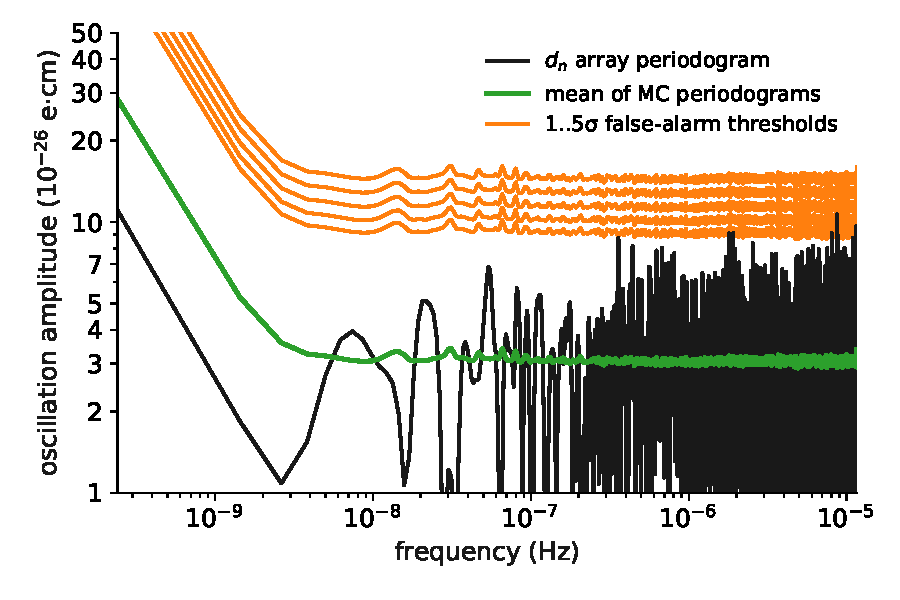
\includegraphics[width=\columnwidth]{gfx/axions/detection_ill.pdf}
  \caption{The periodogram of the array of neutron EDM ($d_\mathrm{n}$) estimates from the ILL measurement (black line).
  We are sensitive to oscillations in the quantity $d_\mathrm{n} - \left( \mu_\mathrm{n} / \mu_\textrm{Hg} \right) \, d_\textrm{Hg}$, where $d_\textrm{Hg}$ is the EDM of the $^{199}$Hg atom. The mean of Monte Carlo (MC)-generated periodograms, assuming no signal is present, is depicted in green. MC is used to deliver false--alarm thresholds (global $p$-values), marked in orange for $1,2,…,5\,\sigma$ levels (from bottom to top). The highest peak has the global $p$\-/value 0.53, consistent with a non-detection.}
  \label{fig:ILL_detection}
\end{figure}

In order to obtain limits on the oscillation amplitude parameter, we again used MC simulations. We discretized the space of possible signals, spanned by their frequency and amplitude. We chose a sparser set of 200 frequencies, as we did not expect highly coherent effects in the sensitivity of detection. For each discrete point, we generated a set of 200 MC
%\note{PMM: perhaps use the words 'toy' or 'sample' instead of fake}
datasets containing the respective, perfectly coherent signal and assumed that the oscillation is averaged over the duration of the run. In general, the sensitivity is phase-dependent, especially for periods comparable with the length of the dataset. For simplicity, we did not investigate the phase-dependence and in the simulation took it to be random and uniformly distributed.
%\note{NA: averaged over run (1 day ish) for ILL, one free precession time for PSI}
% \note{DM: do we need to note that this assumes that the coherence time is at least the length of the run? This is satisfied by the $\Delta f/f\sim 10^{-6}$ width.}
For each fake dataset, we evaluated the LSSA amplitude only at the frequency of the signal and compared its distribution (extrapolating with the functional form of Eq.\,(\ref{eq:powerdistribution})) with the best-fit amplitude in the data and defined the $p$\-/value to be left--sided. We found the 95\% confidence-level exclusion limit as the 0.05 isocontour of the $\mathrm{CL}_s$ statistic \cite{PDG2016}.
The limit is shown as the red curve in Fig.\,\ref{fig:ecm_limits}.
We are most sensitive to periods shorter than the timespan of the dataset ($\sim 4$ years), %\note{NA: we do have good sensitivity down to about 3*10-9Hz or 10 inverse years, but how to phrase this?} (\note{@Nick give a number}), %NA: sensitivity in e cm terms is roughly flat from longer than total measurement time up to individual data point time
% \note{CG: implies to me a 10 year dataset (1998-2002?)}
but rapidly lose sensitivity for periods shorter than the temporal spacing between data points ($\sim 2$ days), since the expected signal would essentially average to zero over these short time scales.

\begin{figure}
  \centering
  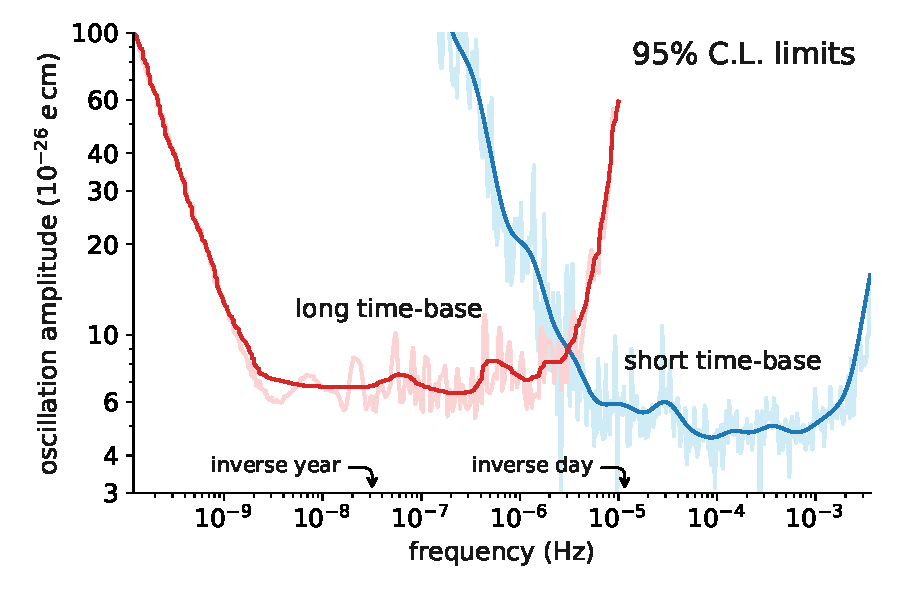
\includegraphics[width=\columnwidth]{gfx/axions/psi_ill_1e-26ecm.pdf}
  \caption{The 95\% C.L. limits on the amplitude of oscillation in the quantity $d_\mathrm{n} - \left( \mu_\mathrm{n} / \mu_\textrm{Hg} \right) \, d_\textrm{Hg}$, as a function of frequency thereof. The limits from the long (ILL data) and short (PSI data) time--base analyses are depicted by the red and blue curves, respectively, with the area above these curves being excluded.
  The raw limits delivered by the analysis, with substantial noise, are depicted by the light lines, while the smoothed versions are given in bold.
  %The PSI data, being more sensitive \note{MR: better formulation?}, deliver stronger limits.
%   \note{MR: Smoothing long time--base such, that it doesn't look systematically shifted?}
%   \note{KK: yes, it looks somehow strangely shifted at the larger slopes on both sides}
%   \note{MR: Proposed solution: smoothing is for visual perception, and this is on a logarithmic scale. Hence, the smoothing (filtering) should be done on the logarithm of the array.}
  %\note{YS: The last sentence sounds awkward here, since the current PSI data appear to only be more sensitive for the higher frequencies. I think the lower baseline for the PSI dataset (which will extend to lower frequencies given enough time for more data collection) is already evident from the graph, so perhaps there is no need to (over)state the obvious here?}
  % \note{MR: Comment on the losses of sensitivity? Comment on why is the short time--base lower (more statistics)?}
  % \note{YS: Strictly, these are constraints on the combination of parameters $d_n - (\gamma_n/\gamma_{\textrm{Hg}}) d_{\textrm{Hg}}$. While we are mainly sensitive to the $d_n$ part of this combination when we consider the axion's coupling to the gluons, in principle Hg might give a non-negligible contribution in other (not yet hypothesised) DM models that produce oscillating EDMs. As an aside, in the case of the axion-wind effect (not an oscillating EDM), Hg gives quite a large contribution.}
  % \note{MR: I fully agree. I think it is important enough to write a short paragraph about it.}
  % \note{Mr: Comment on the different scaling of noise and signal in power spectra.}
  }

  \label{fig:ecm_limits}
\end{figure}

% \note{MR: Try to make the transition ILL -> PSI only once, so that the reader is not confused. Below first describe the changes made to the ILL apparatus and why, as motivation, they enable going to the short time--base analysis.}

\section{Short time-base analysis}
In 2009, the Sussex--RAL--ILL apparatus was moved to the new ultracold neutron source at the Paul Scherrer Institute (PSI), Villigen, Switzerland~\cite{Anghel2009,Lauss2011,Lauss2012,Lauss2014}, where a number of improvements were made~\cite{Baker2011,Afach2015USSA,Ban2016NANOSC}. In 2015, the apparatus was fully commissioned and began to take high-sensitivity EDM data. The whole data set, taken from August 2015 until the end of 2016, with a higher accumulated sensitivity than the ILL one, was considered in this analysis. For the PSI experiment's data, we performed a lower--level oscillation search on the array of $R$ measurements. Since an $R$ estimate was obtained every cycle ($\unit[\approx 300]{s}$), rather than every 1--2 days as for a $d_\mathrm{n}$ estimate, it has an increased sensitivity to higher frequencies. Additionally, the analysis could benefit from the addition of 16 atomic cesium vapor magnetometers \cite{Knowles2009, Koch2015},
% \note{KK: Add 2 references here: P. Knowles et al., NIMA 611, 306 (2009); S. Afach et al., EPJD 69, 225 (2015).}
located directly above and below the precession chamber (inside the electrodes). This made it possible to account for the dominant time--dependent systematic effect on a cycle, rather than run, basis.
% \note{GP: State already here, that there is higher sensitivity. This is the motivation to have two different analyses. In addition, we have the Cs magnetometers, which allows... (In ILL we saw, that there are no significant drifts of the gradient. Even if there are, these are accounted for by increasing the error-bar. The HV reversal is to be able to correct for gradient fluctuation.)}

The dominant time-dependent systematic effect, encapsulated in $\Delta$ of Eq.\,\eqref{eq:R}, would have given rise to non-statistical temporal fluctuations if not accounted for. Namely, $R$ is sensitive to drifts in the vertical gradients of the magnetic field. While the thermal mercury atoms filled the chamber homogeneously, the center of mass of the ultracold neutron population was lower by several millimeters~\cite{Afach2014magmoment, Afach2015, Pendlebury2015}.
%\note{KK: Add 2 more references here: S. Afach et al., PRL 115, 162502 (2015); S. Afach et al., PRD 92, 052008 (2015).}
% \note{MR: This can be added, if needed. The additional contribution to $R$ is: \note{MR: the explicit equation may be left out, if we need space.}
% \begin{equation}
%   \label{eq:deltah}
%   \Delta_{\Delta h} = \mp \Delta h \left[ \frac{\nu_n}{\nu_\textrm{Hg}} \,
%     \frac{1}{B} \left( G_{1,0} - \frac{3 r^2}{4} G_{3,0} \right) \right] \,
% \end{equation}
% where $G_{1,0}$ and $G_{3,0}$ are cubic and linear vertical gradients of the magnetic field \note{MR: cite the paper about the formalism (Guillaume Pignol}.}
To evaluate the correction, the drifts of the gradients were estimated on a cycle basis by fitting a second--order parametrization of the magnetic field to the measurements of the cesium magnetometers~\cite{WurstenThesis}. The center-of-mass shift was determined to be \unit[4]{mm} using the method described in \cite{Afach2014magmoment}.

% The gradients were estimated by fitting a third--order parametrization of the magnetic field to the measurements of the cesium magnetometers. In the time between the runs the magnetometers were operated in a so-called variometer mode, giving a vector information about the magnetic field \note{MR: cite Elise's thesis (not published yet)}. These measurements were used to estimate $\Delta h = \unit[4]{mm}$ (a method analogous to \cite{Afach2014magmoment}). Gradients estimated during runs, when only the vertical component was measured, were used to evaluate \eqref{eq:deltah} and correct for it.

% The caesium magnetometers, located above and below the precession chamber, measured the vertical gradient of the magnetic field. With the gradient measurement, it is possible to perform a lower--level oscillation search on the array of $R$ measurements in the PSI experiment.
% \note{GP, TL, DR: We feel that the statement about importance of the Cs magnetometers for the analysis is too strong.
% It it implicitly written that the short time base analysis is in principle impossible without online control of the gradient.
% It gives the impression that the ILL data cannot probe the high frequency at all, and access to short time oscillation is made possible at PSI only due to the addition of Cs magnetometers.
% In reality, the highest frequencies (above $10^5$ Hz) do not really benefit from any significant improvement using the online gradient correction, only the frequencies around the inverse day are blurred by the G drift.
% We suggest to change the argument page 3 right column, the transition paragraph between the ILL analysis and the PSI analysis.
% Instead of insisting on the addition of Cs, we should insist on the fact that the instantaneous sensitivity (i.e. the cycle sensitivity) has increased.
% The fact that the Cs allow to attenuate the low frequency drifts is just nice but it is not essential, since for frequencies lower than the E field reversal frequency one could analyses the EDM time series instead of the R time series as in the long time-base. }
% \note{MR: Plot the periodogram of not-gradient drift corrected data, too? This would show where the correction actually matters.}
% Although the determination of the ratio $R$ is insensitive to drifts in the magnetic field, it is sensitive to drifts in the vertical gradient of the magnetic field, $\partial B_z / \partial z$. This is because the thermal mercury atoms fill the chamber homogeneously, while the center of mass of the ultracold neutron population is several millimetres lower \cite{Afach2014magmoment}. The exact value of this shift... An ongoing investigation... How it translates to variations in $R$ for various types of magnetic field drifts. We took it to be \unit[3.3]{mm}.
% \note{MR: Needs motivation and explanation. Need to talk to Elise.}
% \note{GP, TL, DR: As a reference for the gravitational shift ref [56] (spin echo paper) is cited. It is true that the spin echo signal would not exist without the grav shift, but here we are referring to the shift of the UCN frequencies averaged over UCN energy bins, for which the spin echo technique is insensitive by principle. We should cite the direct measurement S. Afach et al. Phys. Lett. B 739 (2014) 128 Also, could you indicate what value of the CM offset h you used?}

The measurement procedure involved working deliberately with gradients affecting $R$ (see the crossing--point method in \cite{Pendlebury2015}). Those intended gradients (up to \unit[60]{pT/cm} in \unit[10]{pT/cm} steps) were much larger than cycle--to--cycle fluctuations (\unit[< 2]{pT/cm} per day). With the high-order shifts in $R$ having been significant, these large shifts could not be corrected using the cesium magnetometers. Additionally, while the cesium magnetometers were precise, their accuracy is limited by the calibration procedure. We defined as a \emph{sequence} a set of data, typically 2--3 days in duration, without a deliberate change in the magnetic-field gradient or a recalibration of the cesium magnetometers.
% On the other hand, the precise, but not accurate, cesium magnetometers can only measure the change of the gradient. We need to assume a new random offset in the measurement each time the magnetometers are recalibrated. \note{JK: Why do we recalibrate?} We define as a \emph{sequence} a set of data, typically 2--3 days in duration, without a renewal of the calibration.
% \note{EW: Regarding the sequences in the short time-base dataset. It is technically correct that each sequence is defined by a calibration of the CsMs, but even if we would not calibrate each time when we start a run, you would still have to split based on changes in the magnetic field configuration (R shifts due to G3,0, $<Bt^2>$ and GPE, which is not compensated for with the CsM correction).}
When performing the LSSA fit, we allowed the free offset to be different in each sequence:
\begin{equation}
	% A\sin(2 \pi f t) + B\cos(2 \pi f t) + C_1\,\Pi_1(t) + C_2\,\Pi_2(t) + \ldots \,
    A\sin(2 \pi f t) + B\cos(2 \pi f t) + \sum_i C_i\,\Pi_i(t) \, ,
\end{equation}
where $C_i$ is the free offset in the $i^\textrm{th}$ sequence and $\Pi_i(t)$ is a gate function equal to one in the $i^\textrm{th}$ sequence and zero elsewhere.
% \note{FP: I am a bit confused why have all the constants C in the equation. Should this not read like:  $A\sin(2 \pi f t) + B\cos(2 \pi f t) + C_i$  and then you fit each region with a different $C_i$. Now it is written as if all the offsets add up to a total offset of $C_1 + C_2 + C_3 + \ldots$ }
% \note{MR: Fair point. In fact each $C_i$ is actually $C_i \cdot g_i(t)$, where $g_i(t)$ is a gate function, one in $i$th sequence and zero elsewhere.}
This caused the short time--base analysis to lose sensitivity for periods longer than one sequence.
It should also be mentioned that, at the time of this analysis, the PSI data were still blinded, whereby an unknown, but constant, $d_\mathrm{n}$ was injected into them. It does not influence this analysis, as the free offsets are not considered further.
% \note{PSW: It is not so relevant that the offset are free parameters of the fit (A and B are too), but that the fitted offsets are not further used in the rest of the analysis, as we are only interested in the AC part of the signal.}

% To allow for compensation of systematic effects \note{cite false edm paper(s)}, between runs the magnetic field configuration, and in particular the vertical gradient was changed. This causes a change in the ratio of neutron and mercury Larmor precession frequencies due to gravity shifting down the centre of mass of the slow neutrons compared with that of the relatively fast cohabiting mercury atoms.

% Both experiments yield one $d_n$ estimate per so-called \emph{run}, which consists of many Ramsey measurements in all three field configurations ($\vtr{E}$ and $\vtr{B}$ parallel, anti-parallel and no electric field). The $d_n$ is estimated...  \note{Maybe move it to the beginning of the ILL analysis description}. This limits.
% However, one can go to shorter time--scales if one analyses the array of ratios of the neutron and mercury \note{the comagnetometer must be introduced at this point} precession frequency instead, which is obtained around every 300 seconds. This observable still includes various systematic effects. In particular, it is susceptible to drifts of the magnetic-field gradient, due to the center-of-mass height difference between the neutron and mercury ensembles. One of the improvements in the PSI experiment is the addition of Cs vapour magnetometers below and above the precession volume. They make it possible to correct for the gradient fluctuations.

% Now write about fitting different offset. The following, aside from the true nEDM signal, affect $R$. The offset changes due to the gradient drifts. It is corrected with the Cs magnetometers. Every 2-3 days the gradient deliberately set in the apparatus (to enable interpolation to zero-gradient) is changed, causing a sudden change in $R$. Cs magnetometers calibration alters the intrinsic offset of each magnetometer (they are not accurate), causing a jump, too. We define as \emph{sequence} a set of data without a deliberate change in the magnetic field and without renewal of the calibration. When doing the LSSA fit we allow the free offset $C$ to be different in each sequence. \note{MR: Mention that the data were blinded, too.}
% \begin{equation}
% 	A\sin(2 \pi f t) + B\cos(2 \pi f t) + C_1 + C_2 + \ldots
% \end{equation}
% where $C_i$ is the free offset in $i$th sequence \note{MR: really call it a sequence}

We split the $R$ time array into three sets:
% A control set is data taken without an applied electric field.
% There are two sets that are sensitive to an oscillating EDM, namely the sets with the applied electric and magnetic fields parallel and antiparallel.
a control set of data without an applied electric field, and two sets sensitive to an oscillating EDM, namely with parallel and antiparallel applied electric and magnetic fields.
% \note{CG: Might be good to say what the standard sequence is: 48 at HV, 8 at zero}
% \note{PSW: A control set of data without applied electric field, and two sets sensitive to an oscillating EDM, namely with parallel and antiparallel applied electric and magnetic fields.}
A coherent oscillating EDM signal would have an opposite phase in the latter two sets, and be absent in the control set.
We did not perform a common fit. Instead, the two sensitive data sets were treated separately in the LSSA fits, and later combined to a limit. Otherwise, the LSSA treatment was the same as in the long time--base analysis. We picked a set of $156\,198$ trial frequencies, spaced apart at intervals determined by the spectral resolution
%\note{PSW: Is that correct English? "spaced every spectral"}
%\note{YS: Maybe ``spaced apart at intervals determined by the spectral resolution''?}
(the inverse of 506 days = $\unit[23]{nHz}$), which here also defines the signal width.

The periodogram of the $R$ time array taken with the parallel-field configuration is shown in black in Fig.\,\ref{fig:PSI_detection}.
There are two regions of expected rise in the oscillation amplitude due to the time structure of the data collection.
The one around $\unit[28]{\upmu Hz}$ (the inverse of 10 hours) corresponds to the period of the electric-field reversal.
The very narrow one around $\unit[3.3]{mHz}$ (the inverse of $\unit[300]{s}$) corresponds to the cycle repetition rate.
There are five
%\note{NA does anybody know what style guide says about when numbers should be written in words i.e. seven vs 7? I personally think small numbers without units should be words but this comes down to preference} ***I THINK LESS THAN TEN IT IS IN WORDS - MALCOLM ***
trial frequencies for which the $3\sigma$ false--alarm threshold is exceeded,
%\note{PMM: use words like 'surpassed', or 'exceeded' instead of penetrated}
two of which, including the largest excess with a $6\sigma$ significance, occur in a $\unit[100]{\upmu Hz}$ region around the inverse of \unit[300]{s}, while the other three are in the low-frequency region (inverse days) already excluded by the long time--base analysis.
% \note{FP: Can you maybe also explicitly state the positions of these three lines in Hz or inverse time?}
 The periodograms for the other two datasets (not shown) are very similar.
In the other sensitive set, there are three excesses of the $3\sigma$ threshold (the highest is $5\sigma$), all constrained to the same two regions. In the control dataset, only the $1\sigma$ threshold is exceeded.
%\note{MR: We may consider not discussing the false--alarm threshold penetrations, and just state in the next paragraph that we do not find a signal which meets our criteria.}
The periodogram of the $R$ time array without the gradient-drift correction is shown in pink in Fig.\,\ref{fig:PSI_detection} to visualize the frequencies where the correction has an effect.

\begin{figure}
  \centering
  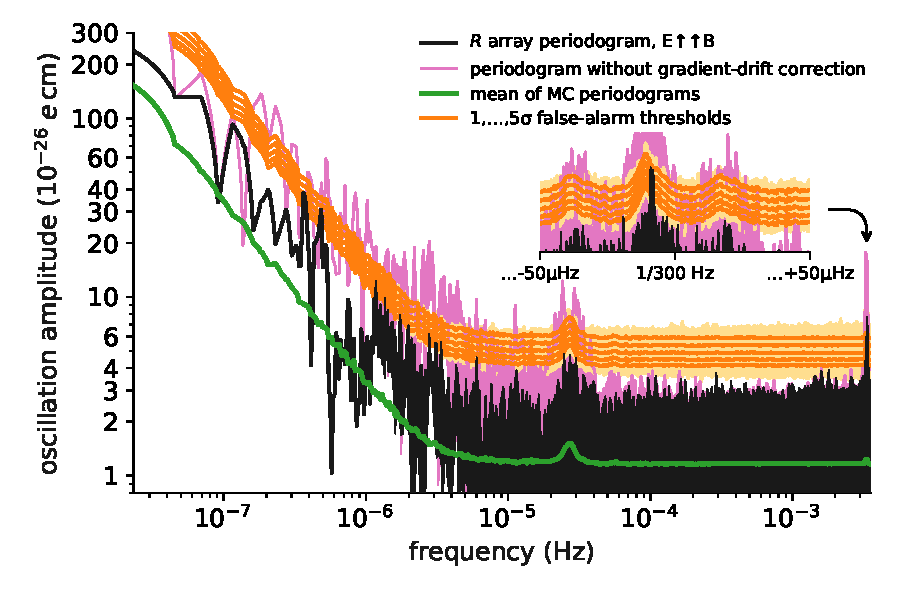
\includegraphics[width=\columnwidth]{gfx/axions/detection_psi_inset_gc.pdf}
  \caption{
  Periodogram of the $R$ time array of the PSI experiment data, sensitive to oscillations in the quantity $d_\mathrm{n} - \left( \mu_\mathrm{n} / \mu_\textrm{Hg} \right) \, d_\textrm{Hg}$, taken with the $\vtr{E}$ and $\vtr{B}$ fields parallel (black line).
  The mean of MC--generated periodograms, assuming no signal, is depicted in green. MC is used to calculate $1,2,…,5\,\sigma$ false--alarm thresholds, depicted in light orange.
  % \note{YS: It's a bit difficult to see the yellow on this graph. Or perhaps yellow means light orange here?}
  For clarity, we also plot the smoothed version in orange.
  %As they are noisy, a smoothed version is plotted on top in orange.
  There are two regions where a rise in the amplitude is expected, namely around $\unit[28]{\upmu Hz}$ (inverse of 10 hours) and $\unit[3.3]{mHz}$ (inverse of 300 seconds), due to the time structure of the data taking (see the main text for more details). The periodogram of non-gradient-drift-corrected data is shown in pink.
  % \note{MR: Maybe for the PRL it would be good not to show the narrow peak? Just to trim the frequency range a bit. It would save a lot of explanations, but I don't know if we can do that.}
  % \note{MR: comment on filtering of the limits and on the inset (remind the cycle repetition rate: 300s.}
%   \note{YK: how do you get periodogram values above 1/300s for the short-time base? (I would expect a really sharp end of the period. there)}
  % \note{JZ: in both the main text and figure caption you use 3.3 mHz. Maybe it will be less confusing to place in the x-axis of the inset 3.3 mHz instead of 1/300 Hz}
%   \note{JZ: one of three data sets is presented here. Which one? It is not written, I am afraid. I think it would be much more convincing if you will show Fig 3 at least for two data sets because you are not able to give exact reasons for some observed picks. There are some speculations only. If these picks exist in data sets collected with and without electric field it would helpful to understand these speculations. It is better to the reader to see it and not only to read about it.}
  }
  \label{fig:PSI_detection}
\end{figure}

A non--statistical excess in a periodogram of $R$ may be caused not only by a coherent oscillating signal;
for example, fluctuations of a higher--order term in the magnetic field, not compensated by either the mercury or cesium magnetometers, may cause broad--band elevations in LSSA power.
% \note{MMM: The previous sentence is long and hard to follow.  I suggest rewording.}
% This was not a problem in the long time--base analysis, where the manner in which each $d_n$ estimate was obtained ensured correlation with the relative orientation of the electric and magnetic fields, rejecting all uncorrelated fluctuations.
% \note{MR: explain that the data is low level. Point to a possible source of non-statistical behaviour? E.g. In particular, a careful study of the Caesium magnetometer array is still ongoing. Or say that the analysis is ongoing. But not give the impression that we show a work-in-progress analysis.}
We defined strict requirements for an excess to be considered as one induced by axion DM as follows.
Firstly, a significant ($>3\sigma$) excess in amplitude had to be observed in both sensitive datasets at the same frequency, but not in the control set. Secondly, the signals must be in antiphase in the parallel and anti-parallel datasets. Lastly, we require high coherence (a narrow peak) equal to the spectral resolution of the dataset. None of the significant excesses passed our discovery criteria.
%\note{DM: did you also need to use the fact that some peaks were excluded by the long-time base analysis, or does the PSI data independently exclude all of the excesses based on these criteria? MR says PSI independently excludes peaks so make sure we say this.}
% \note{GP, TL, DR:
% In the paragraph where we apologize for these peaks, there is a sentence "This was not a problem in the long time-base analysis, where the manner in which each $d_n$ estimate was obtained ...." We believe it is not correct.  For high frequency noise (higher than the E field reversal frequency) the averaging over the cycles do not suppress the extra noise.  In this case we would see an increased of the power in the periodogram for each frequency. We suggest to remove this sentence.
% Beside giving excuses, what did we do to try to understand the origin of these significant peaks?
% To go in this direction we insist it is of utmost importance to perform the periodogram analysis of the west timeseries to see if these peaks are there too. }
% \note{MR: The analysis of the Western data is ready, waining for response...}

We delivered a limit on the oscillation amplitude similarly to the long time--base analysis, with the exception that we required the product of the two sensitive sets' $\mathrm{CL}_s$ statistics to be 0.05.
The limit is shown as the blue curve in Fig.\,\ref{fig:ecm_limits}.
With the short time--base analysis, we were most sensitive to periods shorter than the timespan of a sequence (2 -- 3 days), and lost sensitivity to periods shorter than the cycle repetition rate ($\approx 5$ minutes).
The PSI dataset has a higher accumulated sensitivity than the ILL dataset, so the limit baseline in the sensitive region is slightly better in the case of the PSI dataset.

Following Eq.\,(\ref{eq:nEDM_axion}), we can interpret the limit on the oscillating neutron EDM as limits on the axion--gluon coupling in Eq.\,(\ref{Axion_couplings}).
We present these limits in Fig.\,\ref{fig:axion_limits_v2}, assuming that axions saturate the local cold DM energy density $\rho_{\mathrm{DM}}^{\mathrm{local}} \approx 0.4~\textrm{GeV/cm}^3$ \cite{Catena2010}.
%\note{GP: DM experiments chose to use the value of 0.3 GeV, and it is pessimistic on purpose. Need to answer! }
%\note{YS: The current (and several previous) Particle Data Group reviews on DM have consistently quoted the value $0.4~\textrm{GeV}/\textrm{cm}^3$, presumably because this value represents the mean of the various independent determinations of the DM densities in our local galactic neighbourhood. I'm not saying that $0.3~\textrm{GeV}/\textrm{cm}^3$ is an incorrect value (after all, it lies within the range of possible values), but I think the pessimistic/conservative approach is not justified in the present case, because from independent observations of planetary orbits within the Solar System (which importantly do not contradict larger-scale determinations of the DM density) the density of DM on Earth and hence in laboratory experiments can be up to 6 orders of magnitude larger than the quoted value $0.4~\textrm{GeV}/\textrm{cm}^3$; see, e.g., https://arxiv.org/abs/astro-ph/0601422 }
Our peak sensitivity is
%\note{YS: Based on Fig.~4, I would have expected something closer to $f_a/C_G \approx 10^{21}$ GeV}
% \note{YS: The figure indicates a number close to $f_a/C_G \sim 10^{21}$ GeV, rather than $10^{-21}$ GeV$^{-1}$, which is for the reciprocal quantity $C_G/f_a$. It seems reasonable to give the sensitivity here to 1 digit of significance, i.e. $f_a/C_G \approx y \times 10^{zz}$ GeV. }
$f_a/C_G \approx \unit[1 \times 10^{21}]{GeV}$ for $m_a \lesssim \unit[10^{-23}]{eV}$, which probes super-Planckian axion decay constants ($f_a > M_{\textrm{Planck}} \approx 10^{19}~\textrm{GeV}$), that is, interactions that are intrinsically feebler than gravity.
%\note{JK: axion coupling does go $1/r^2$?}\note{DM: yes, but it also has a term proportional to the dot-product of the spins, and a Yukawa suppression for the axion mass. Here I read this as referring rather to the energy scale of suppression of terms in an effective field theory, regardless of the specific type of force they mediate.}
%\note{YS: We could in principle avoid having to say most of this, if we follow your (and my) suggestion in the figure caption to simplify the constraints graph to include only our nEDM results and the existing BBN constraints. If we do this, then we should still explain the $\sqrt{\rho}$ scaling of the constraints (either in the caption or in the text).}
%\note{YS: By the way, Doddy, where do you see the 4 orders of magnitude improvement in Fig.~4? (It's possible that we could be seeing different renderings of the graph in our viewers, since for me the dotted line corresponding to the Planck scale at $f_a \approx 10^{19}$ GeV appears to be shifted a bit upwards compared with where I would expect to see it. In this case, we should compare the nEDM and BBN limits using the raw number from the [@Nick] part above.}

% To search for the axion-wind effect, Eq.~(\ref{potential_axion-wind}), we partitioned the entire PSI dataset into two sets with opposite magnetic-field orientations (irrespective of the electric field) and then analyzed the ratio $R = \nu_\mathrm{n} / \nu_\textrm{Hg}$ similarly to our oscillating EDM analysis above.

\section{Axion-wind effect}
We also perform a search for the axion-wind effect, Eq.\,(\ref{potential_axion-wind}), by partitioning the entire PSI dataset into two sets with opposite magnetic-field orientations (irrespective of the electric field) and then analyzing the ratio $R = \nu_\mathrm{n} / \nu_\textrm{Hg}$ similarly to our oscillating EDM analysis above.
The axion-wind effect would manifest itself through time-dependent shifts in $\nu_\mathrm{n}$ and $\nu_\textrm{Hg}$ (and hence $R$) at three angular frequencies:~$\omega_1 = m_a$, $\omega_2 = m_a + \Omega_{\textrm{sid}}$ and $\omega_3 = |m_a - \Omega_{\textrm{sid}}|$, with the majority of power concentrated in the $\omega_1$ mode.
Also, the axion-wind signal would have an opposite phase in the two subsets.
We find two overlapping $3\sigma$ excesses in the two subsets (at $\unit[3.42969]{\upmu Hz}$ and $\unit[3.32568]{mHz}$), neither of which have a phase relation consistent with an axion-wind signal.
Following Eq.\,(\ref{potential_axion-wind}), we derive limits on the axion-nucleon coupling in Eq.\,(\ref{Axion_couplings}).
We present these limits in Fig.\,\ref{fig:axion_limits_v2}, assuming that axions saturate the local cold DM energy density.
Our peak sensitivity is
$f_a/C_N \approx \unit[4 \times 10^{5}]{GeV}$ for $\unit[10^{-19}]{eV} \lesssim m_a \lesssim \unit[10^{-17}]{eV}$.

\section{Conclusions}
In summary, we have performed a search for a time-oscillating neutron EDM in order to probe the interaction of axion-like dark matter with gluons.
We have also performed a search for an axion-wind spin-precession effect in order to probe the interaction of axion-like dark matter with nucleons.
So far, no significant oscillations have been detected, allowing us to place limits on the strengths of such interactions.
Our limits improve upon existing astrophysical limits on the axion-gluon coupling by up to 3 orders of magnitude and also improve upon existing laboratory limits on the axion-nucleon coupling by up to a factor of 40.
Furthermore, we constrain a region of axion masses that is complementary to proposed ``on-resonance'' experiments in ferroelectrics \cite{CASPEr2014}. Future EDM measurements will allow us to probe even feebler oscillations and for longer periods of oscillation that correspond to smaller axion masses.

% \note{FP: Just a questions concerning your conclusions. You say: "future EDM measurements will allow us to probe even feebler oscillations and for longer periods of time\ldots" Concerning the second point - when you "combine" the ILL and PSI data, can you not make exclusions around the inverse time of 15 years. This would be the approx. time between the two experiments (ILL: 1998-2002 / PSI: 2015-2016).}
% \note{MR: We could theoretically do it, but first we would need to have a free offset in fit to PSI data (blinding) and second, most importantly, we would need to use an array of $d_n$ estimates from PSI data, which is essentially doing the nEDM analysis. We should either comment on why we don't combine the data (to greatly simplify the analysis?) or otherwise at least not give an explicit hint that they should have been combined.}

%\note{DM: The nEDM data can also be used to search for the anomalous spin-precession induced by the ``axion wind'' coupling $g_N$ \cite{Flambaum2013Patras,Stadnik2014A,Graham2013} with an approximate sensitivity to  $f_a/C_N=g_N^{-1}\sim 10^{6}\text{ GeV}$ over our frequency range. The appropriate analysis of the data is ongoing.}
%\note{YS: It would be even nicer if we could also present the axion-wind results in this paper :)}


%\begin{figure}
%  \centering
%  \includegraphics[width=\columnwidth]{psi_ill_axion_limits.pdf}
%  \caption{
%  	\note{MR: The exact scope and content of this plot needs to be discussed and agreed on.}
%  	\note{MR: Description to be added.}  \note{MR: I put a version like this in Fig.\,\ref{fig:axion_limits_v2}, so we can look at both for now.}}
%  \label{fig:axion_limits}
%\end{figure}

\begin{figure}
  \centering
  \includegraphics[width=\columnwidth]{gfx/axions/psi_ill_axion_limits_v7.pdf}
  \includegraphics[width=\columnwidth]{gfx/axions/psi_ill_axion_wind_limits_v1.pdf}
  \caption{
  %\note{YS: Extend the upper y limit from $10^{-4}$ to $10^{-2}$ in order to make the plot more symmetric and give a larger visual `buffer zone' for the supernova limits.}
  %\note{YS: Change ``super-Planckian $f_a$'' label to ``super-Planckian axion decay constant'', and change ``CASPEr'' to ``CASPEr (projected)''. }
  %\note{YS: Perhaps extend lower y limit from $10^{-22}$ to $10^{-24}$, to give the nEDM limits a bit more breathing room.}
  %\note{YS: Mostly a question of taste, but I generally find labels on the graph and the axes labels which start with a capital letter to be more appealing to the eye (except for nEDM in this case).}
  %\note{Needs refinement of label positions.}
%  \note{Add axion-nucleon constraints graph underneath axion-gluon constraints graph. Maybe can focus on the region: $10^{-22} eV < m_a < 10^{-17} eV$ and $10^2 GeV < C_N/f_a < 10^{10} GeV$, or similar. The three regions to plot in this case would be our n/Hg constraints (same colour as for nEDM constraints), laboratory searches for new spin-dependent forces (yellow), and supernova energy-loss bounds (green).}
%\note{Update bottom graph to match format of top graph.}
%\note{KK: For bottom figure, it would be nice to have the same colour everywhere for our limits (like the top graph) - perhaps it could be dashed and through that one would still see the yellow and green parts?}
%\note{KK: For bottom figure, extend the upper mass a bit (maybe to $\sim 10^{-16}$ eV?), so that we see our limit becoming less sensitive again than the yellow exclusion.}
% \note{YS: Is it possible to check the positioning of the horizontal dashed line (corresponding to the Planck scale) in the top figure? The Planck scale corresponds to $C_G/f_a \approx 10^{-19}~\textrm{GeV}^{-1}$, while the current dashed horizontal line looks like it is a bit high. }
% \note{YS: On the bottom figure, change font of subscript labels in $\nu_n/\nu_{Hg}$ to be $\nu_\textrm{n}/\nu_\textrm{Hg}$, like in main text.}
Limits on the interactions of an axion with the gluons (top) and nucleons (bottom), as defined in Eq.\,(\ref{Axion_couplings}), assuming that axions saturate the local cold DM content.
  The regions above the thick blue and red lines correspond to the regions of parameters excluded by the present work at the 95\% confidence level (C.L.).
  The colored regions represent constraints from Big Bang nucleosynthesis (red, 95\% C.L.) \cite{Blum2014,StadnikThesis,Stadnik2015D}, supernova energy-loss bounds (green, order of magnitude) \cite{Graham2013,Raffelt1990Review,Raffelt2008LNP}, consistency with observations of galaxies
  %(orange, \note{@DM: What is the C.L. here?})
  (orange) \cite{Marsh2015Review,Marsh2015B,Schive2015,Marsh2017}, and laboratory searches for new spin-dependent forces (yellow, 95\% C.L.) \cite{Romalis2009_NF}.
  %\note{DM: give approximate C.L. or refer to text for explanation of level of rigour}, and consistency with observations of galaxies (orange) \cite{Marsh2015Review,Marsh2015B,Schive2015,Marsh2017}.
  The nEDM, {\color{black}$\nu_\mathrm{n} / \nu_\textrm{Hg}$} and Big Bang nucleosynthesis constraints scale as $\propto \sqrt{\rho_a}$, while the constraints from supernovae {\color{black}and laboratory searches for new spin-dependent forces} are independent of $\rho_a$.
  The constraints from galaxies are relaxed if axions constitute a sub-dominant fraction of DM.
  We also show the projected reach of the proposed CASPEr experiment (dotted black line)~\cite{CASPEr2014}, and the parameter space for the canonical QCD axion (purple band).
%   \note{DM: y-axis should be $\sqrt{\rho}$}
%   \note{YS: Actually, I suggest to remove $\rho_a$ altogether from the y-axis label, since the QCD axion and Super-Planckian regions are $\rho_a$-indepedent, as too are the supernova energy-loss bounds. The scaling of the constraints is in fact already explained in the caption above: we state that the constraints assume saturation of DM by axions (which is correct for all of the regions on the graph), then we proceed to state that the nEDM and BBN constraints scale as $\propto{\sqrt{\rho_a}}$, so that the reader will have in mind the $\propto{\sqrt{\rho_a}}$ implicitly on the y-axis for these constraints.}\note{DM: okay, but if we assume saturation of DM then some (even dotted or mild line) for galaxies should go in?}
%\note{KK: a comment on 'Super-Planckian' is missing.}
%\note{YS: I have now added a brief comment on this in the main text.}
% \note{PH: our lines need to go up to the top of the plot.  There has to be a division between excluded and not excluded regions.}
% \note{YS: (Depending on the changes proposed above,) for aesthetics, could we perhaps shift the "Super-Planckian axion decay constant" label downwards? And perhaps also shift the "long time-base" label down and to the left, and shift the "short time-base" label down and a bit to the left?}
}
\label{fig:axion_limits_v2}
\end{figure}


\section{END the PRX paper}





\section{Motivation}


\section{Theoretical background}


\section{Time series construction}

\subsection{nEDM @ PSI data taking scheme}
The nEDM experiment at PSI probes the Ramsey resonance curve of ultra--cold neutrons (\emph{UCNs}). Its operation consists of subsequent \emph{cycles}, wherein an ensemble of polarised \emph{UCNs} undergoes a Ramsey cycle in a magnetic field. At the end the polarisation of the ensemble is measured. The measurement is performed in a controllable electric field, which takes up three values: parallel to the magnetic field, antiparallel to it and zero. The electric field configuration is altered every couple of tens of cycles.

The Ramsey resonance curve of the neutrons is probed only in four \emph{working points}, as shown in Fig.\,\ref{fig:axions_working_points}. The points lie on the curve's steep slope. Thereby the resonance position is determined more precisely then it would should the curve be probed homogeneously or close to the resonance.

\begin{figure}[bth]
  \myfloatalign
  \subfloat
  [The \emph{working points} method. The plot depicts the measured neutron polarisation in function of the $pi/2$ pulses frequency. The frequencies are normalised by appropriate gyromagnetic ratios.]
  {\includegraphics[width=.45\linewidth]{gfx/axions/data_taking_working_points}}
  \quad
  \subfloat
  [The \emph{working points} are probed subsequently.]
  {\label{fig:example-b}
  \includegraphics[width=.45\linewidth]{gfx/axions/data_taking_working_points_time}}
  \caption{The principle of working points}
  \label{fig:axions_working_points}
\end{figure}

The resonance frequency $f_n^{\,0}$ is determined with a fit of the resonance curve. Because the points are probed one after another, it is only possible after a set of data points, \emph{cycles}, have been measured. In order to extract the neutron precession frequency for each individual \emph{cycle}, one assumes that the only parameter of the resonance curve that varies on a cycle--to--cycle basis is the position of the resonance. With this assumption the shape of the curve, fitted to the whole set of \emph{cycles}, is used to calculate back the resonant frequency in each \emph{cycle} of the set.

Together with the UCNs there is a polarised $^{199}$Hg gas precessing. Its precession is monitored with light, allowing for direct determination of the $^{199}$Hg Larmor frequecy and thus the magnetic field strength. In order to cancel the first-order magnetic field changes one looks at the value:
\begin{equation}
  R := f_n / f_{Hg} \ .
\end{equation}
However, the UCNs are cold enough to have their centre of mass shifted downwards a few centimeters by the gravity. The $^{199}$Hg gas, being much hotter then the UCNs, fills the precession volume homogeneously. In a presence of a vertical magnetic field gradient this causes the two species to see different magnetic fields.

In the nEDM experiment at PSI data taking is divided into \emph{runs}. A single \emph{run} is carried out automatically with, in most cases, no human intervention. The machine cycles through the working points by itself. Also the charging of the electrodes creating the electric field is automatised. In between \emph{runs} manual interference happens, most importantly the magnetic field vertical gradient is altered.

In order to mitigate the bias due to the human factor, the nEDM experiment implements \emph{data blinding}. The data is artificially altered in a way that mimics a non--zero neutron electric dipole moment, big enough to be visible in the data. The exact value is secret and will be revealed only after the analysis is complete.


\subsection{An oscillating nEDM signal}
The main purpose of the experiment is to measure the constant neutron electric dipole moment. This would appear as a shift in $R$ dependent on the electric field. Zero electric field would cause no shift, while the parallel and anti--parallel configurations of the magnetic and electric fields would shift $R$ in opposite directions. Due to the \emph{data blinding} the shift is expected even in case of zero nEDM.

Should the neutron electric dipole moment oscillate, $R$ would oscillate as well. Even if the electric field is kept constant. A reversal of the electric field polarity would change phase of the oscillations by $\pi$. At zero electric field no oscillations would be visible. The effect is depicted in Fig.\,\ref{fig:axions_data_taking_one_run}.

\begin{figure}[bth]
  \myfloatalign
  \subfloat
  [An oscillating neutron electric dipole moment signal in the nEDM @ PSI apparatus. The colours indicate different electric field states: parallel to the magnetic field, antiparallel to it and zero]
  {\label{fig:axions_data_taking_one_run}
  % \includegraphics[width=.34\linewidth]{gfx/axions/data_taking_run}}
  \includegraphics[width=.34\linewidth]{gfx/axions/data_taking_run_with_blinding}}
  \quad
  \subfloat
  [An oscillating neutron electric dipole moment signal in the nEDM @ PSI apparatus across many runs. The colours indicate different electric field states: parallel to the magnetic field, antiparallel to it and zero. Different runs have different magnetic field gradients, which causes each run to have a different shift in $R = f_n / f_{Hg}$.]
  {\label{fig:axions_data_taking_runs}
  \includegraphics[width=.56\linewidth]{gfx/axions/data_taking_runs}}
  \caption{The data taking scheme in the nEDM experiment at PSI.}
\end{figure}

The vertical magnetic filed vertical gradient changes when a new \emph{run} is started. Thereby $R$ is shifted by a big value, changing the DC level of the oscillating nEDM signal, which is illustrated in Fig.\,\ref{fig:axions_data_taking_runs}. Moreover, even during a single \emph{run} the gradient drifts, as clearly visible in Fig.\,\ref{fig:axions_gradient_drift}.

The nEDM team spares no effort to measure the gradient. Nevertheless, the achieved precision ($\approx \unit[1]{pT/cm}$ is only comparable to the one of $f_n$ (in the order of \unit[1]{pT}). The exact way how the gradient should determined is highly non--trivial and there is ongoing research in this respect. Actually, even the height difference between the neturons and $^{199}$Hg centres of mass (a few milimeters) is still discussed. % Assuming a constant gradient during a \emph{run} one can determine it much more precise. This assumption, however, is known not to be exactly true.

\begin{figure}[bth]
  \myfloatalign
  \includegraphics[width=.8\linewidth]{gfx/axions/gradient_drift_yoann}
  \caption
  [Drift of $R$]
  {%FIXME directly copied from Yoann's presentation on the 2015 PSI collaboration meeting
A typical time series of $R$ in the nEDM experiment. The colours depict electric field states, black being no electric field. A drift is clearly visible.}
  \label{fig:axions_gradient_drift}
\end{figure}

One should note, that any, including an oscillating one, nEDM effect affects only the position of the neutrons' resonance. The shape of the resonance curve is unaffected. Therefore, the method to extract neutron Larmor frequency $f_n$, and thereby $R$, for each \emph{cycle} is valid also in case of an oscillating nEDM.


\subsection{$R$ time series demodulation}
The time series of $R$ is not eligible for a Fourier--type analysis. The series has to be first demodulated into a coherent signal. To accound for the electric field changes, data taken at one configuration need to be \emph{flipped} around the DC level. Unfortunately, determining the DC level is not trivial.

Taking a look at Fig.\,\ref{fig:axions_gradient_drift} it becomes clear, that the $R$ value drifts. The main reason is a drift of the vertical gradient of the magnetic field. This effect could corrected for using the gradient measurement, as shown in Fig.\,\ref{fig:axions_gradient_drift_correction}. It is not straightforward, though, as there is not yet an established method to determine the gradient. The points taken at zero electric field provide additional information about the DC level. This, however, would have to be interpolated. The gradient drift correction is likely to turn out to be the most delicate part of the analysis.

\begin{figure}[bth]
  %FIXME directly copied from Elise's presentation on the 2015 PSI collaboration meeting
  \myfloatalign
  \subfloat
  [Another time series of $R$ in the nEDM experiment. The colours depict electric field states, black being no electric field. A drift is clearly visible.]
  {\label{fig:axions_gradient_drift_not_corrected}
  \includegraphics[width=.45\linewidth]{gfx/axions/gradient_drift_elise}}
  \quad
  \subfloat
  [The data as on Fig.\,\ref{fig:axions_gradient_drift_not_corrected} corrected for gradient fluctuations.]
  {\label{fig:axions_gradient_drift_corrected}
  \includegraphics[width=.45\linewidth]{gfx/axions/gradient_drift_elise_corrected}}
  \caption{Correcting the $R$ time series for fluctuations of the vertical magnetic field gradient.}
  \label{fig:axions_gradient_drift_correction}
\end{figure}

% The gradient drift correction is likely to turn out to be the most delicate part of the analysis. One could consider two methods of tackling the problem. Firstly, the electric field configurations could be separated and analysed separately. In this case no correction for the gradient drift is necessary, although it
%
% Because of drift - not trivial to correct.
% Two analyses:
% 1. + and - HV separately -- the highest freqency is twice slower, but no correction necessary, but still possible. Gradient drift mimics a signal though.
% 2. try to correct for gradient and combine the data into one array


\section{Time series analysis}
\subsection{Definition of the periodogram}
The analysis starts with calculating \emph{the periodogram}, an estimator of the power spectral density, of the demodulated $R$ time series. Therefor an array of $N$ frequencies $\omega_i$ is chosen. For each a linear least--squares fit is performed with a model:
\begin{equation}
  R(t) = A\ \mathrm{sin}\,\omega t + B\ \mathrm{cos}\,\omega t \ .
\end{equation}
Then the power at the frequency $\omega$ is defined:
\begin{equation}
  P(\omega) = \frac{N}{4} \, (A^2 + B^2)\ .
\end{equation}
The definition is similar to the one used by \citeauthor{VanTilburg2015}~\citep{VanTilburg2015}, but uses normalisation as defined by \citeauthor{Scargle1982}~\citep{Scargle1982}. One should remember, that the periodogram is an estimator. Its statistical properties are thoroughly described by \citeauthor{Scargle1982}~\citep{Scargle1982}.


\subsection{Null hypothesis test}
Once the periodogram of the real data, demodulated $R$ time series, is calculated we look for a signal. A signature of a periodic signal is a peak in the periodogram. The really interesting statement is the answer to the question:

\begin{center}
  \emph{How likely it is, that the highest peak in the periodogram cannot be only a random fluctuation?}
\end{center}

To describe the question mathematically, let us denote the time series from the real data by $D$. The peridogoram is then a set of $P^D(\omega_i)$. We are interested in \emph{the maximum of the periodogram}:
\begin{align}
  P_{max}^D &:= \mathrm{max}_i\,P^D(\omega_i) \\
  \omega_{max}^D &:= \mathrm{arg\,max}_i\,P^D(\omega_i)
\end{align}
The height of the maximum, $P_{max}^D$, is a random variable. We consider the distribution of $P_{max}$ given the null hypothesis, $H_0$, where an array of normally distributed random variables is taken. The probability that a peak at least as high as the one observed arises as a random fluctuation is:
\begin{equation}
  \mathrm{Pr}\left( P_{max} > P_{max}^D\ |\, H_0 \right) \ .
\end{equation}
This value is called the \emph{false alarm probability} (see eg. \citeauthor{Pandola2004}~\citep{Pandola2004}). It can be numerically calculated with a Monte--Carlo method by generating random data according to the null hypothesis and counting the relative number of cases when $P_{max} > P_{max}^D$. To claim a discovery the \emph{false alarm probability} has to be at most in the range of $10^{-7}$ (so--called 5--sigma).

It should be stressed that the distribution of $P_{max}$ is very different from the distribution of $P(\omega_{max})$. The highest peak will always occur in a far tail of the $P(\omega_{max})$ distribution, which is natural. By looking for the highest peak we check a big number of random variables $P(\omega_i)$ and pick the one that does lie the furthest in the tail of the distribution. The distribution of $P_{max}$ is centered around much higher values, as the highest peak is bound to occur \emph{somewhere}. It is explained in Fig.\,\ref{fig:axions_null_rejection}.

\begin{figure}[bth]
  \myfloatalign
  \includegraphics[width=.8\linewidth]{gfx/axions/axionMC_null_rejection}
  \caption
  [...]
  {
Testing not--yet--real data against the null hypothesis. \textsc{Upper--left:} The periodogram of the data (black line) on top of the periodogram of the null hypothesis (green line with Monte--Carlo generated distribution bands). \textsc{Upper--right:} The distribution of $P(\omega_{max})$, given the null hypothesis (vertical slice through the green part of the plot in the upper--left corner). \textsc{Lower--left:} CDF of $P(\omega)$ evaluated at $P^D(\omega)$ in function of $\omega$. \textsc{Lower--right:} The distribution of $P_{max}$. }
  \label{fig:axions_null_rejection}
\end{figure}


\subsection{Signal hypotheses tests}
Should no claim for a discovery be possible, the next question to ask is:
\begin{center}
  \emph{Which oscillations would produce a visible peak, but did not, and can be thus excluded?}
\end{center}
In order to answer this question, the data need to be tested against being compatible with a number of model signal hypotheses. As an oscillation is characterised by its amplitude and frequency, the space of the hypotheses to test is two--dimensional.

The probability that a hypothetical oscillation of amplitude $A$ and frequency $\omega$ would produce more power at $\omega$ then observed is:
\begin{equation}
  \mathrm{Pr}\left( P(\omega) > P^D(\omega)\ |\, H(\omega, A) \right) \ .
\end{equation}
This probability is the \emph{confidence level} (C.L.) at which the hypothesis $H(\omega, A)$ can be rejected. Figure\,\ref{fig:axions_signal_rejection} presents comparing a not--yet--real data power spectrum with a hypothetical signal. This test may be performed many times, each covering a \emph{pixel} of the space of possible hypotheses, forming an image as in Fig.\,\ref{fig:axions_exclusion}. The set of hypotheses excluded at a certain C.L. (often 95\%) forms an \emph{exclusion region}.

\begin{figure}[bth]
  \myfloatalign
  \includegraphics[width=.8\linewidth]{gfx/axions/axionMC_signal_hypothesis_rejection}
  \caption
  [...]
  {
\textsc{Left:} A periodogram of not--yet--real data on top of distribution of a periodogram of a hypothetical signal (green). \textsc{Right:} The distribution of power of the hypothetical signal at its model frequency.}
  \label{fig:axions_signal_rejection}
\end{figure}

\begin{figure}[bth]
  %FIXME directly copied from Elise's presentation on the 2015 PSI collaboration meeting
  \myfloatalign
  \subfloat
  [The not--yet--real data tested against hypothetical signals. Each pixel is one signal hypothesis. The white line connects points of 95\% C.L., surrounding an exclusion region. Note how deep into low amplitudes the line goes for couple of frequencies. See the text for the explanation.]
  {\label{fig:axions_exclusion}
  \includegraphics[width=.45\linewidth]{gfx/axions/axionMC_exclusion}}
  \quad
  \subfloat
  [The not--yet--real data tested against hypothetical signals using the \emph{CLs method}, in which hypotheses to which the experiment is not sensitive to get a statistical penalty. ]
  {\label{fig:axions_exclusion_CLs}
  \includegraphics[width=.45\linewidth]{gfx/axions/axionMC_exclusion_CLs}}
  \caption{Exclusion region --- signals that can be excluded at 95\% confidence level.}
  \label{fig:axions_exclusions}
\end{figure}

The exclusion region, depicted by a white line in Fig.\,\ref{fig:axions_exclusion}, is exhibits a number of thin peaks going down in very low amplitudes. Seemingly for some frequencies signals with amplitude far below the sensitivity of the experiment are excluded. This is disturbing. Consider, however, that as the power was evaluated for many frequencies, inevitably at some of them, roughly 5\%, the power is low enough to be rejected at 95\%~C.L. even when tested against a white noise. However completely fine from the statistical point of view, physicists do not accept a situation, where a hypothesis is rejected based on an experiment which was not sensitive to it. One possible solution is called the \emph{CLs method}. The method is defined, as well the problem itself discussed, in the booklet of Particle Data Group~\citep{Group2014}. With use of the \emph{CLs method} the exclusion final region is obtained, as shown in Fig.\,\ref{fig:axions_exclusion_CLs}.


\section{Dedicated measurement}
One could consider performing a dedicated measurement for the ALP search. With a short, more densely sampled measurement one could explore the high mass (thus high frequency) region of possible axions, as was done eg. by \citeauthor{VanTilburg2015}~\citep{VanTilburg2015}.

The measurement would not need to last longer then a day. More dense sampling is possible by shortening the length of a \emph{cycle}. One should note that this worsens at the same time the sensitivity of the measurement. The lowest possible period of measurement in the nEDM apparatus is around \unit[100]{s}.

\section{Results}
